\documentclass[]{article}
\usepackage{lmodern}
\usepackage{amssymb,amsmath}
\usepackage{ifxetex,ifluatex}
\usepackage{fixltx2e} % provides \textsubscript
\ifnum 0\ifxetex 1\fi\ifluatex 1\fi=0 % if pdftex
  \usepackage[T1]{fontenc}
  \usepackage[utf8]{inputenc}
\else % if luatex or xelatex
  \ifxetex
    \usepackage{mathspec}
    \usepackage{xltxtra,xunicode}
  \else
    \usepackage{fontspec}
  \fi
  \defaultfontfeatures{Mapping=tex-text,Scale=MatchLowercase}
  \newcommand{\euro}{€}
\fi
% use upquote if available, for straight quotes in verbatim environments
\IfFileExists{upquote.sty}{\usepackage{upquote}}{}
% use microtype if available
\IfFileExists{microtype.sty}{%
\usepackage{microtype}
\UseMicrotypeSet[protrusion]{basicmath} % disable protrusion for tt fonts
}{}
\usepackage[margin=1in]{geometry}
\ifxetex
  \usepackage[setpagesize=false, % page size defined by xetex
              unicode=false, % unicode breaks when used with xetex
              xetex]{hyperref}
\else
  \usepackage[unicode=true]{hyperref}
\fi
\hypersetup{breaklinks=true,
            bookmarks=true,
            pdfauthor={},
            pdftitle={caRpools - End-To-End Analysis of Pooled CRISPR/Cas9 Screens},
            colorlinks=true,
            citecolor=blue,
            urlcolor=blue,
            linkcolor=magenta,
            pdfborder={0 0 0}}
\urlstyle{same}  % don't use monospace font for urls
\usepackage{color}
\usepackage{fancyvrb}
\newcommand{\VerbBar}{|}
\newcommand{\VERB}{\Verb[commandchars=\\\{\}]}
\DefineVerbatimEnvironment{Highlighting}{Verbatim}{commandchars=\\\{\}}
% Add ',fontsize=\small' for more characters per line
\usepackage{framed}
\definecolor{shadecolor}{RGB}{248,248,248}
\newenvironment{Shaded}{\begin{snugshade}}{\end{snugshade}}
\newcommand{\KeywordTok}[1]{\textcolor[rgb]{0.13,0.29,0.53}{\textbf{{#1}}}}
\newcommand{\DataTypeTok}[1]{\textcolor[rgb]{0.13,0.29,0.53}{{#1}}}
\newcommand{\DecValTok}[1]{\textcolor[rgb]{0.00,0.00,0.81}{{#1}}}
\newcommand{\BaseNTok}[1]{\textcolor[rgb]{0.00,0.00,0.81}{{#1}}}
\newcommand{\FloatTok}[1]{\textcolor[rgb]{0.00,0.00,0.81}{{#1}}}
\newcommand{\ConstantTok}[1]{\textcolor[rgb]{0.00,0.00,0.00}{{#1}}}
\newcommand{\CharTok}[1]{\textcolor[rgb]{0.31,0.60,0.02}{{#1}}}
\newcommand{\SpecialCharTok}[1]{\textcolor[rgb]{0.00,0.00,0.00}{{#1}}}
\newcommand{\StringTok}[1]{\textcolor[rgb]{0.31,0.60,0.02}{{#1}}}
\newcommand{\VerbatimStringTok}[1]{\textcolor[rgb]{0.31,0.60,0.02}{{#1}}}
\newcommand{\SpecialStringTok}[1]{\textcolor[rgb]{0.31,0.60,0.02}{{#1}}}
\newcommand{\ImportTok}[1]{{#1}}
\newcommand{\CommentTok}[1]{\textcolor[rgb]{0.56,0.35,0.01}{\textit{{#1}}}}
\newcommand{\DocumentationTok}[1]{\textcolor[rgb]{0.56,0.35,0.01}{\textbf{\textit{{#1}}}}}
\newcommand{\AnnotationTok}[1]{\textcolor[rgb]{0.56,0.35,0.01}{\textbf{\textit{{#1}}}}}
\newcommand{\CommentVarTok}[1]{\textcolor[rgb]{0.56,0.35,0.01}{\textbf{\textit{{#1}}}}}
\newcommand{\OtherTok}[1]{\textcolor[rgb]{0.56,0.35,0.01}{{#1}}}
\newcommand{\FunctionTok}[1]{\textcolor[rgb]{0.00,0.00,0.00}{{#1}}}
\newcommand{\VariableTok}[1]{\textcolor[rgb]{0.00,0.00,0.00}{{#1}}}
\newcommand{\ControlFlowTok}[1]{\textcolor[rgb]{0.13,0.29,0.53}{\textbf{{#1}}}}
\newcommand{\OperatorTok}[1]{\textcolor[rgb]{0.81,0.36,0.00}{\textbf{{#1}}}}
\newcommand{\BuiltInTok}[1]{{#1}}
\newcommand{\ExtensionTok}[1]{{#1}}
\newcommand{\PreprocessorTok}[1]{\textcolor[rgb]{0.56,0.35,0.01}{\textit{{#1}}}}
\newcommand{\AttributeTok}[1]{\textcolor[rgb]{0.77,0.63,0.00}{{#1}}}
\newcommand{\RegionMarkerTok}[1]{{#1}}
\newcommand{\InformationTok}[1]{\textcolor[rgb]{0.56,0.35,0.01}{\textbf{\textit{{#1}}}}}
\newcommand{\WarningTok}[1]{\textcolor[rgb]{0.56,0.35,0.01}{\textbf{\textit{{#1}}}}}
\newcommand{\AlertTok}[1]{\textcolor[rgb]{0.94,0.16,0.16}{{#1}}}
\newcommand{\ErrorTok}[1]{\textcolor[rgb]{0.64,0.00,0.00}{\textbf{{#1}}}}
\newcommand{\NormalTok}[1]{{#1}}
\usepackage{longtable,booktabs}
\usepackage{graphicx,grffile}
\makeatletter
\def\maxwidth{\ifdim\Gin@nat@width>\linewidth\linewidth\else\Gin@nat@width\fi}
\def\maxheight{\ifdim\Gin@nat@height>\textheight\textheight\else\Gin@nat@height\fi}
\makeatother
% Scale images if necessary, so that they will not overflow the page
% margins by default, and it is still possible to overwrite the defaults
% using explicit options in \includegraphics[width, height, ...]{}
\setkeys{Gin}{width=\maxwidth,height=\maxheight,keepaspectratio}
\setlength{\parindent}{0pt}
\setlength{\parskip}{6pt plus 2pt minus 1pt}
\setlength{\emergencystretch}{3em}  % prevent overfull lines
\providecommand{\tightlist}{%
  \setlength{\itemsep}{0pt}\setlength{\parskip}{0pt}}
\setcounter{secnumdepth}{5}

%%% Use protect on footnotes to avoid problems with footnotes in titles
\let\rmarkdownfootnote\footnote%
\def\footnote{\protect\rmarkdownfootnote}

%%% Change title format to be more compact
\usepackage{titling}

% Create subtitle command for use in maketitle
\newcommand{\subtitle}[1]{
  \posttitle{
    \begin{center}\large#1\end{center}
    }
}

\setlength{\droptitle}{-2em}
  \title{caRpools - End-To-End Analysis of Pooled CRISPR/Cas9 Screens}
  \pretitle{\vspace{\droptitle}\centering\huge}
  \posttitle{\par}
  \author{}
  \preauthor{}\postauthor{}
  \date{}
  \predate{}\postdate{}


% Redefines (sub)paragraphs to behave more like sections
\ifx\paragraph\undefined\else
\let\oldparagraph\paragraph
\renewcommand{\paragraph}[1]{\oldparagraph{#1}\mbox{}}
\fi
\ifx\subparagraph\undefined\else
\let\oldsubparagraph\subparagraph
\renewcommand{\subparagraph}[1]{\oldsubparagraph{#1}\mbox{}}
\fi

\begin{document}
\maketitle

{
\hypersetup{linkcolor=black}
\setcounter{tocdepth}{4}
\tableofcontents
}
\newpage

\begin{center}
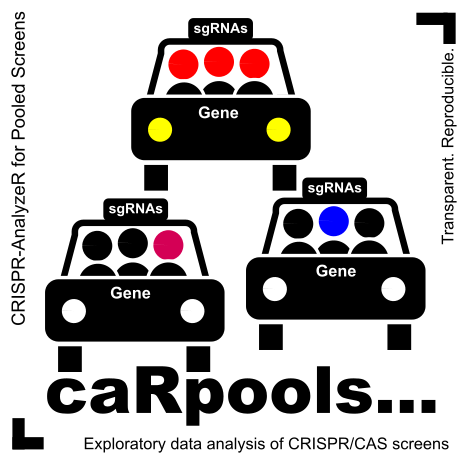
\includegraphics{./pictures/CaRpools.png}
\end{center}

\newpage

\section{Introduction}\label{introduction}

The \textbf{CaRpools} (\textbf{C}RISPR \textbf{A}nalyze\textbf{R} for
\textbf{Pool}ed \textbf{S}creens) package allows users to analyse raw
NGS readcount data from pooled CRISPR Screens in an end-to-end fashion
and serves as a basis for creating customized reports for more advanced
users.\\
These pooled screens must contain lentivirus-based libraries as they can
be obtained via
\href{https://www.addgene.org/CRISPR/libraries/}{Addgene} e.g. . It
provides functions to create different quality control plots, normalize
the data, compare the data and perform hit identification via three
different methods.\\
Furthermore it can be used to completely analyze the date in a
stream-lined workflow with the provided analysis template.

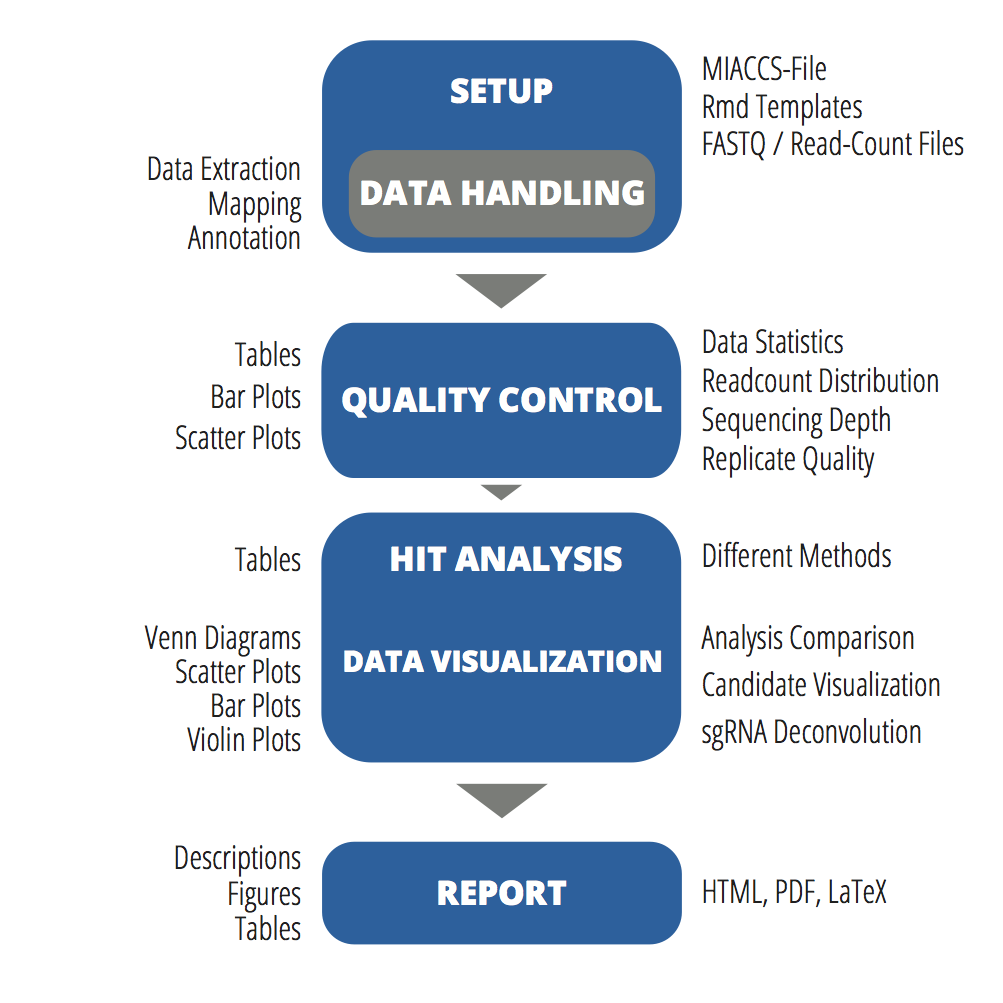
\includegraphics{./pictures/workflow.png}

With \textbf{CaRpools}, the user can analyze pooled CRISPR/Cas9 screens
end-to-end in a standardized fashion allowing for reproducible data
analysis.\\
This includes:

\begin{itemize}
\tightlist
\item
  FASTQ data extraction (optional)
\item
  Mapping against a reference library FASTA file using bowtie2
  (optional)
\item
  Extract Mapping data and convert it into read count files (optional)
\item
  Generate quality control plot
\item
  Generate dataset statistics
\item
  Perform hit analysis using three different methods
\item
  Visualize hit candidates
\item
  Compare hit analysis for most robust hit identification
\item
  Retrieve information about single sgRNAs for hit candidates
\item
  Generate standardized reports, which are fully customizable (for
  advanced users)
\end{itemize}

\newpage

\subsection{Download caRpools}\label{download-carpools}

CaRpools is avaible as an R package \textbf{caRpools} without the
scripts and template files.\\
The complete package with the PERL scripts and all template files can be
obtained from \href{https://github.com/boutroslab/carpools}{Github}
(\url{https://github.com/boutroslab/carpools}) and our website
\href{http://www.crispr-analyzer.de}{CRISPR-AnalyzeR.de}.

We recommend to download the template files and Scripts from Github and
install caRpools in R using the package installer
`install.packages(``caRpools'').

\subsection{Quality Control}\label{quality-control}

Available Quality Control plots include (for sgRNAs or summarized for
genes):

\begin{itemize}
\tightlist
\item
  Readcount Distribution \texttt{carpools.read.distribution}
\item
  Read Depth \texttt{carpools.read.depth}
\item
  sgRNAs present per Gene Target \texttt{carpools.reads.genedesigns}
\item
  Readcount Overview per sgRNA / Gene \texttt{carpools.read.ballmap}
\item
  Readcount comparison of different samples
  \texttt{carpools.read.count.vs}
\item
  Readcount / Foldchange of sgRNAs for single genes
  \texttt{carpools.raw.genes}
\end{itemize}

\subsection{Annotation}\label{annotation}

Since several gene identifiers are used for generating CRISPR pooled KO
libraries, e.g.~EnsemblID,\\
loaded datasets can automatically be annotated with further gene
annotation like official gene symbol or descriptions\\
using the \texttt{biomaRt} interface.\\
More details can be found below in the section of \texttt{get.gene.info}
or via \texttt{?get.gene.info} / \texttt{?biomaRt}.

\subsection{Gene Read Count Data or Removing Gene
Data}\label{gene-read-count-data-or-removing-gene-data}

Furthermore, sgRNA readcount data can be aggregated (summed up) to
corresponding genes \texttt{aggregatetogenes} or gene data can be
excluded for the analysis using \texttt{gene.remove}.

\subsection{Hit Analysis}\label{hit-analysis}

Moreover, this package can be used to identify screening hits using
either

\begin{itemize}
\tightlist
\item
  DESeq2 \texttt{stat.DESeq}
\item
  Wilcox-based hit calling \texttt{stat.wilcox}
\item
  MAGeCK \texttt{stat.mageck}
\end{itemize}

and hit calling / data analysis can be compared between all the methods
with \texttt{compare.analysis} or \texttt{plot.hit.overview}. Finally
evaluated data analysis can be visualized in different ways with
\texttt{carpools.hitident} for all methods listed above.

\subsection{sgRNA Information}\label{sgrna-information}

Moreover, you will also be provided with in-depth information about the
sgRNAs of your genes.\\
These can be derived from \texttt{carpools.raw.genes} for any gene or
\texttt{carpools.hit.sgrna} for your hit candidates in an automated way.

\subsection{Report}\label{report}

All this data can be used to automatically generate a standardized
report using the provided R Markdown termplate file including all plots
and tables for you data analysis.\\
Two different templates are provides:

\begin{itemize}
\tightlist
\item
  A standard report for generating short, brief data anlysis
\item
  An extended report with additional plots and tables
\end{itemize}

The R Markdown templates provide the user with the ability to generate
HTML output as well as PDF output (LATEX installation necessary)
including high-quality plots.

\textbf{Provided PDF templates:}

\begin{itemize}
\tightlist
\item
  CaRpools-PDF.rmd
\item
  CaRpools-extended-PDF.rmd
\end{itemize}

\textbf{Provided HTML templates:}

\begin{itemize}
\tightlist
\item
  CaRpools-HTML.rmd
\item
  CaRpools-extended-HTML.rmd
\end{itemize}

\newpage

\section{Requirements and
Installation}\label{requirements-and-installation}

\subsection{Virtual Box Image}\label{virtual-box-image}

We also included a VirtualBox Image that already includes all necessary
software and package files.\\
You just need to install VirtualBox 5 from the
\href{https://www.virtualbox.org}{Website}.

You can download the caRpools virtual box image from our website
\href{http://www.crispr-analyzer.de}{crispr-analyzer.de} or
\href{https://github.com/boutroslab/carpools}{Github}
(\url{https://github.com/boutroslab/carpools}).

\subsubsection{How to use the Virtual Box
caRpools}\label{how-to-use-the-virtual-box-carpools}

Please see the
\href{https://github.com/boutroslab/caRpools/blob/master/docs/CaRpools-SHORTGUIDE-VirtualBox.Rmd}{VirtualBox
tutorial} for instructions.

\subsection{Download caRpools}\label{download-carpools-1}

CaRpools is avaible as an R package \textbf{caRpools} without the
scripts and template files.\\
The complete package with the PERL scripts and all template files can be
obtained from \href{https://github.com/boutroslab/carpools}{Github}
(\url{https://github.com/boutroslab/carpools}) and our website.

We recommend to download the template files and Scripts from Github and
install caRpools in R using the package installer
`install.packages(``caRpools'').

\subsection{Hardware Requirements}\label{hardware-requirements}

For CRISPR-Libraries of 12 K size (12K sgRNAs), caRpools will work on
any laptop/PC with at least 4GB of RAM and a modern dual-core CPU.\\
CRISPR-Libraries with a size of more than 100 K (100 K sgRNAs) run best
with at least 8 GB of RAM.

\subsection{Software Requirements}\label{software-requirements}

CaRpools was tested on MacOSX Yosemite and Ubuntu 14.04 LTS.\\
However, it should work on any operating system that fulfills the
software requirments.

The following software needs to be installed:

\begin{itemize}
\tightlist
\item
  PERL 5
\item
  Bowtie2 2.2.0 or higher
  \href{http://bowtie-bio.sourceforge.net/bowtie2/index.shtml}{Website}
\item
  MAGeCK 0.51 (password protected download)
  \href{http://sourceforge.net/p/mageck/wiki/Home/}{Website}
\item
  TexLive \href{https://www.tug.org/texlive/}{Website}
\item
  pdflatex
\item
  xelatex
\item
  R 3.2.0 or higher \href{https://www.r-project.org/}{Website}
\item
  Pandoc 1.15.0.6 \href{http://www.http://pandoc.org/}{Website}
\item
  R-Studio \href{http://www.rstudio.com}{Website} (GUI)
\end{itemize}

The following \textbf{R packages} need be installed (can be done via
\texttt{load.packages()}):

\begin{itemize}
\tightlist
\item
  Bioconductor Basics

  \begin{itemize}
  \tightlist
  \item
    BiocInstaller \textgreater{}= 1.18.3
  \item
    BiocGenerics \textgreater{}= 0.14.0
  \end{itemize}
\item
  \textbf{biomaRt \textgreater{}=2.24.0}
\item
  seqinr \textgreater{}= 3.1-3
\item
  xlsx \textgreater{}= 0.5.7
\item
  rJava \textgreater{}= 0.9.6
\item
  xlsxjars \textgreater{}= 0.6.1
\item
  stringi \textgreater{}= 0.5
\item
  scatterplot3d \textgreater{}= 0.3
\item
  MESS \textgreater{}= 0.3
\item
  DESeq2 \textgreater{}= 1.8.1
\item
  rmarkdown \textgreater{}= 0.7
\item
  knitr \textgreater{}= 1.10.5
\item
  VennDiagram \textgreater{}= 1.6.9
\item
  sm \textgreater{}= 2.2
\end{itemize}

\subsection{BiomaRt and Annotation
Requirements}\label{biomart-and-annotation-requirements}

\textbf{Please note that for any annotation, biomaRt needs full access
to the internet.} In case of incorrect proxy settings, the report
generation will fail with a biomaRt error.\\
This means that if any proxy server is used, this has to be configured
before using caRpools as described in the following articles:

\begin{itemize}
\tightlist
\item
  \href{http://www.bioconductor.org/packages/release/bioc/vignettes/biomaRt/inst/doc/biomaRt.pdf}{BiomaRt
  vignette}
\item
  \href{https://support.rstudio.com/hc/en-us/articles/200488488-Configuring-R-to-Use-an-HTTP-Proxy}{Setting
  up proxy in R-Studio}
\item
  \href{http://stackoverflow.com/questions/6467277/proxy-setting-for-r}{Setting
  up proxy in R, Stackoverflow}
\item
  \href{http://askubuntu.com/questions/572722/setting-up-the-proxy-for-rstudio}{Setting
  up Proxy for R/R-Studio in Ubuntu}
\item
  \href{https://bhoom.wordpress.com/2013/05/27/configuring-r-to-use-an-http-proxy-faq-knowledge-base-rstudio-support/}{Configuration
  of Proxy for R}
\end{itemize}

\subsection{Installation Procedure}\label{installation-procedure}

Install all software listed above according to the installation
information stated on the software website.\\
All neccesarry R packages can be installed automatically by
\texttt{load.packages()}.

\subsection{Dataset / Screening
Requirements}\label{dataset-screening-requirements}

Since CaRpools fosters reproducibility of CRISPR/Cas9 screens, the
following requirements for pooled screening data \textbf{must be
fullfilled to analyze data}:

\begin{itemize}
\tightlist
\item
  Two biological replicates of \emph{untreated} sample data
\item
  Two biological replicates of \emph{treated} sample data
\end{itemize}

The usage of more than two replicates at once is not yet implemented,
but will be in the near future.

\subsection{Files that can be loaded}\label{files-that-can-be-loaded}

The following files are required for data analysis:

\textbf{Either}\\
* NGS FASTQ file for each sample * Library reference in FASTA format

\textbf{or}\\
* Final read count file for each sample * Library reference in FASTA
format

CaRpools accepts either FASTQ files or read count files for each sample.
FASTQ file are then extracted and mapped using Bowtie2 against the
library reference. Finally, read count files for each sample are
generated.

As an alternative, these final read count files can be provided as well,
so that no extraction or mapping is necessary.\\
In addition, a library reference file in FASTA format is necessary,
usually this is the file that was used for ordering custom oligo
libraries.

File structures are shown below.

\subsubsection{Structure of NGS Readcount
Data}\label{structure-of-ngs-readcount-data}

General information about the FASTQ file format can be obtained in an
easy-to-understand article from
\href{https://en.wikipedia.org/wiki/FASTQ_format}{Wikipedia}.

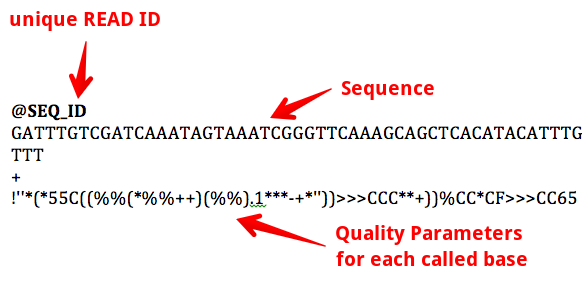
\includegraphics{./pictures/fastq-format.png}

\textbf{maschine.pattern}\\
The maschine pattern used for extracting the sequences is a regular
expression to identify the read ID including your sequencing maschine.\\
in the case of the above sample, the PERL regular expression used must
be \textbf{M01100}.

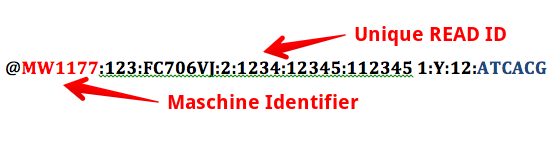
\includegraphics{./pictures/fastq-format-example.png}

\subsubsection{Extraction Pattern}\label{extraction-pattern}

CaRpools extracts the integrated DNA sequence of your target sequence as
a DNA barcode.\\
In order to extract this sequence, a \textbf{PERL regular expression}
pattern is used to identify the desired nucleotide sequence, which is
called \textbf{seq.pattern}.

As an example, part of a U6 promoter-driven sgRNA cassete is given as
follows:

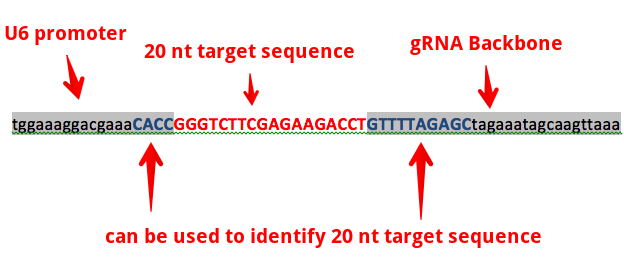
\includegraphics{./pictures/extraction.png}

Since we want to extract the target sequence, the regular expression
will use a part of the U6 promoter and a part of the sgRNA backbone to
identify the target sequence.

CACC \textbf{(.\{20\})} GTTTTAGAGC

The parenthesis are necessary to extract the target sequence, for more
information please see \href{http://www.regexr.com/}{RegExR}.

\subsubsection{Structure of FASTA Library Reference
File}\label{structure-of-fasta-library-reference-file}

The library reference file must be in FASTA format and include ALL
sgRNAs present in the dataset with exactly the same naming.\\
e.g.

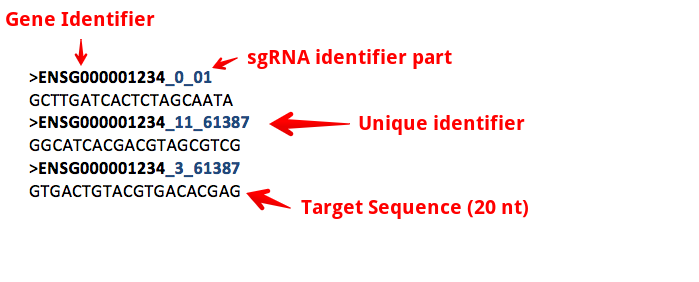
\includegraphics{./pictures/library-fasta.png}

\subsubsection{Read-Count Data Files}\label{read-count-data-files}

CaRpools also takes read count files. If FASTQ files are provided and
extracted/mapped with CaRpools, read count files will be created for
each sample.\\
Data for each sample must be formated in a \textbf{tab-separated} way as
follows:

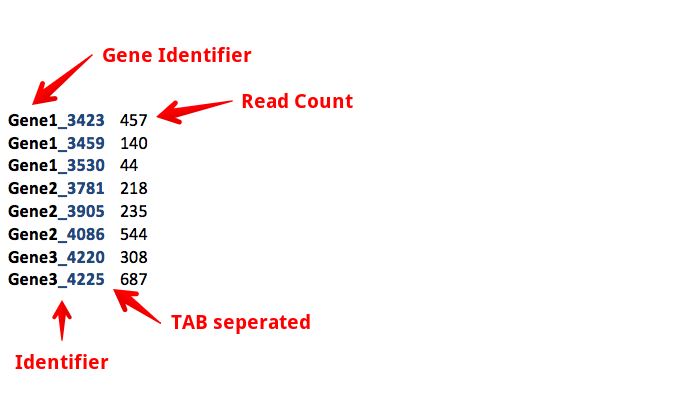
\includegraphics{./pictures/readcount.png}

As shown in the above file, \textbf{Gene1} is the Gene identifier,
**\_3423** is a unique part for identification of this sgRNA for the
given gene and \emph{Gene1\_3423} is the whole identifier which uniquely
identifies this sgRNA within the dataset.

The name of each complete sgRNA \textbf{must} contain the gene it refers
to either as gene symbol or any other identifier which shares the same
separator in addition to a part of identifier that is unique for each
sgRNA for that gene.\\
The name can therefore be anything, as long as the \emph{identifier is
the same for each gene} and the \emph{separator is the same for all
data}.

In principle a sgRNA identifier must consist of a \textbf{gene
identifier}, followed by a \textbf{seperator} (e.g. \_ or -) as well as
a \emph{secondary} \textbf{sgRNA identifier}.

\textbf{Please note:}\\
* Read counts MUST be numeric only. * Within the sgRNA/Gene identifer,
no special characters \emph{except for \_ and -} are allowed!

\subsubsection{File Loading}\label{file-loading}

Files can be loaded via \texttt{load.file(filename,\ header,\ sep)} with
the following arguments

\begin{itemize}
\tightlist
\item
  filename: the filename as character
\item
  header: TRUE / FALSE , whether a header is used (as it is for the
  above sample)
\item
  sep: the seperator, default is \texttt{\textbackslash{}t} for
  tab-separated files.
\end{itemize}

\textbf{Please see \texttt{?read.table} for a detailed description of
the arguments.}

\subsection{Files and Folder Structure to use
CaRpools}\label{files-and-folder-structure-to-use-carpools}

\textbf{Please note: the MAIN FOLDER must be the R working directory!}\\
Data and Script paths can be adjusted in the MIACCS file.

The following files are neccessary to use CaRpools for report
generation:

\textbf{MIACCS.xls}\\
Minimum Information About CRISPR/Cas Screens. This file needs to be
filled out to provide all necessary informations about the screen.

\textbf{R Markdown Template files}\\
Either CaRpools-extended-PDF.rmd, CaRpools-PDF.rmd or
CaRpools-extended-HTML.rmd or CaRpools-HTML.rmd. Is the template for
report generation.

\textbf{Data Files}\\
Two replicates per Control and Treated. Can be FASTQ files OR already
mapped, not normalized read count files.

\textbf{CRISPR-mapping.pl}\\
PERL script to map your extracted FASTQ files, if desired (as indicated
in the MIACCS.xls)

\textbf{CRISPR-extract.pl}\\
PERL script to extract 20 nt target sequence from FAST files, if desired
(as indicated in the MIACCS.xls)

\textbf{CaRpools.png}\\
The logo file

The following files are necessary to use \emph{single} CaRpools
functions:

\textbf{Data Files}\\
Either raw read count files or FASTQ files (that need to be extracted
and mapped using CaRpools)

Please note that CaRpools always starts with loading data files. For
raw-readcount files, use \texttt{load.file}. For FASTQ files, please see
the sections below.

\newpage

\textbf{CaRpools folder structure for Report Generation using raw Read
Count files:}

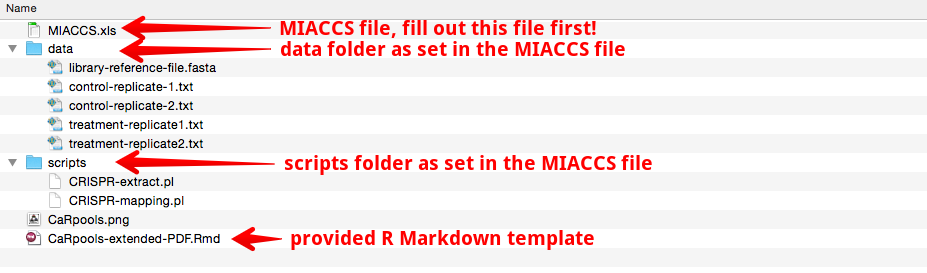
\includegraphics{./pictures/folder-structure-before.png}

\newpage

\textbf{CaRpools folder structure for Report Generation using raw Read
Count files AFTER REPORT GENERATION:}

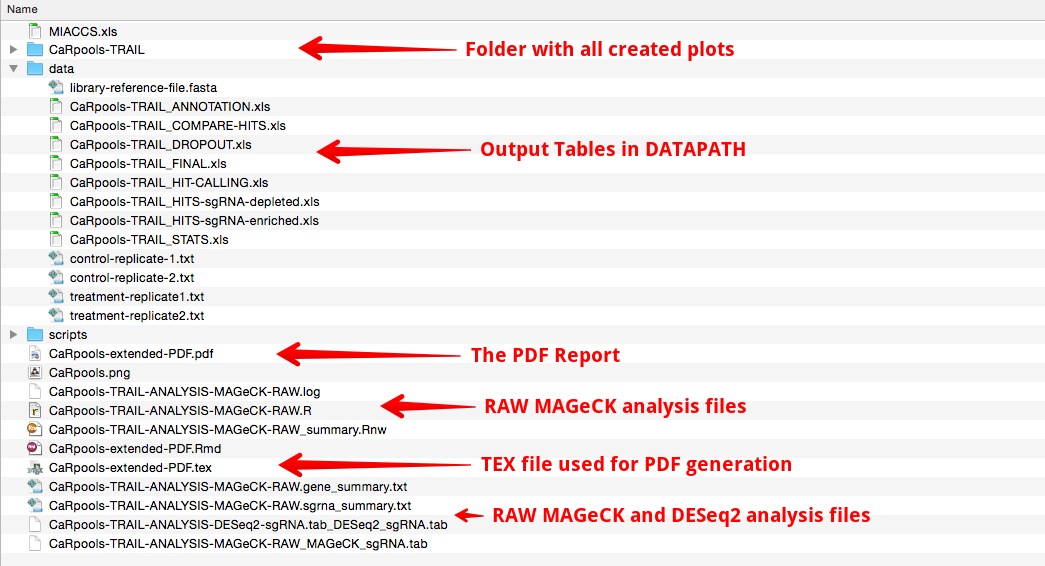
\includegraphics{./pictures/folder-structure-FINAL.png}

\newpage

\textbf{CaRpools folder structrue for Report Generation using FASTQ
files:}

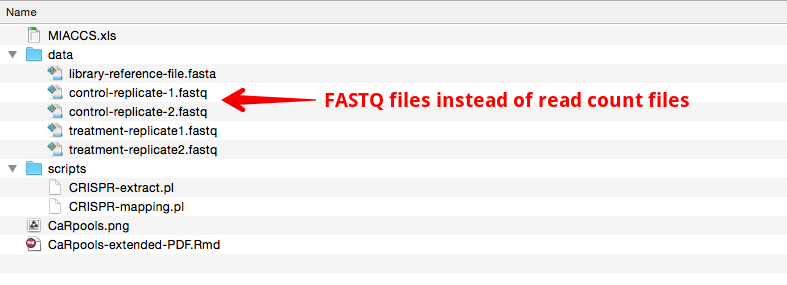
\includegraphics{./pictures/folder-structure-FASTQ-before.png}

\newpage

\textbf{CaRpools folder structure for Report Generation using FASTQ
files AFTER REPORT GENERATION:}

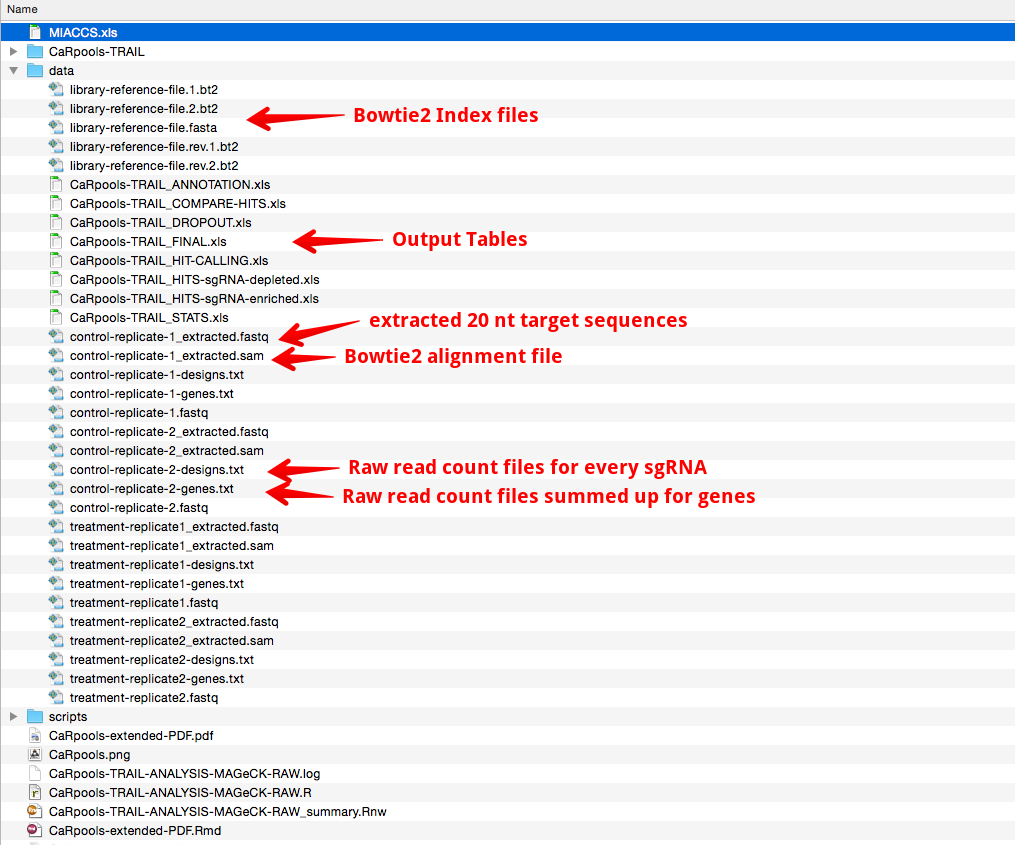
\includegraphics{./pictures/folder-structure-FASTQ-FINAL.png}

\newpage

\section{Using CaRpools with Provided R Markdown
Templates}\label{using-carpools-with-provided-r-markdown-templates}

By default, CaRpools is meant to be used to generate standardized
reports of CRISPR/Cas9 pooled screenings using the provided R markdown
templates.\\
However, these templates can also serve as a basic frame for advanced
users to modifiy them and create customized reports to their needs.

In the following sections, the use of CaRpools with the provided
template files is explained in more detail. Please see the above
instructions of how to install all necessary tools, packages and
components for CaRpools.

For the modification of the templates, please see the manuals for R
Markdown and knitr. Single parameters and detailed instructions of the
single function within CaRpools are given in the section \textbf{Using
CaRpools as a stand-alone R Package}.

\subsection{Setup Files and R-Studio}\label{setup-files-and-r-studio}

All packages and software tools need be installed correctly as shown
before.

\begin{enumerate}
\def\labelenumi{\arabic{enumi}.}
\tightlist
\item
  Copy all files in the designated folders as shown above.
\end{enumerate}

\begin{itemize}
\tightlist
\item
  \textbf{Please note: the MAIN FOLDER must be R working directory!}
\item
  The MIACCS.xls as well the R markdown template and CaRpools.png must
  be in the same folder as the R working dir.
\end{itemize}

\begin{enumerate}
\def\labelenumi{\arabic{enumi}.}
\setcounter{enumi}{1}
\tightlist
\item
  Adjust the path to the data and scripts folder if necessary in the
  MIACCS.xls . Use the absolute path. If the folder structure is as
  shown above, you do not need to make any adjustments.
\item
  Adjust and fill out the \textbf{MIACCS.xls} file.
\item
  You can use \texttt{CarPools(type="check")} to check for the correct
  folder structure and data file presence as it is indicated in the
  MIACCS.xls file.
\item
  You can check for your R working directory by \texttt{getwd()} and set
  it to any directory you want by \texttt{setwd("/PATH")}.
\end{enumerate}

\subsubsection{Check Setup}\label{check-setup}

You can verify that the MIACCS.xls file as well as the used template
file and all necessary scripts are found by calling
\texttt{check.caRpools()}.\\
See below for more information about the arguments.\\
By default, it \textbf{requires a correct MIACCS file + the script files
+ all packages installed + MAGeCK + Bowtie2 + Pandoc.}

\subsection{The MIACCS.xls file}\label{the-miaccs.xls-file}

The MIACCS (\textbf{M}inimum \textbf{I}nformation \textbf{A}bout
\textbf{C}RISPR/\textbf{C}as \textbf{S}creens) file, provided as Excel
sheet, combines all information which is necessary to reproduce the
screens. This includes a description of the screen, hypothesis, all
materials used as well as the experimental workflow.\\
Moreover, the MIACCS file is used to setup the analysis using caRpools,
thus allowing a reproducible and standardized way of performing and
analyzing pooled CRISPR/Cas screens.

The following parameters are found within the MIACCS.xls file:

\subsubsection{Using FASTQ Files}\label{using-fastq-files}

Instead of providing already mapped read count files, caRpools provides
the functionality to use the generated RAW FASTQ files as they are
supplied by the sequencing maschine, e.g.~Illumina MiSeq/NextSeq/HiSeq
systems.\\
If desired, caRpools can extract your 20 nt target sequence (without
filtering for quality) from these files and map it against your library
reference using bowtie2. In this case, you need to provide the following
files that must be within the datapath set in the MIACCS file:

\begin{itemize}
\tightlist
\item
  Two replicate FASTQ files for the untreated sample
\item
  Two replicate FASTQ files for the treated sample
\item
  Your ordered library reference as FASTA file
\item
  optional bowtie2 index files of your library fasta files (generated
  via bowtie2-build)
\end{itemize}

Moreover, the wrapper files CRISPR-mapping.pl and CRISPR-extract.pl need
to be in the scriptpath as set in the MIACCS file.

caRpools will then generate the following files during the extraction
and mapping:

\textbf{filename\_extracted.fastq} FASTQ file with the extracted 20 nt
target sequence\\
\textbf{multiple library-filename.bt2} bowtie2 index files (if create
index files set as TRUE in the MIACCS file)\\
\textbf{filename\_extracted.sam} SAM alignment file of the extracted 20
nt target sequence against the library reference\\
\textbf{filename\_extracted-designs.txt} Read Count files for each
sgRNA\\
\textbf{filename\_extracted-genes.txt} Read Count files SUMMED up for
each gene (not used during analysis)

The following parameters must be set in the MIACCS.cls file under
\textbf{Data Extraction and Bowtie2 Mapping/Alignment} to extract file
from FASTQ data:

\textbf{Do you want to extract the sgRNA target sequence from FASTQ?}
\emph{TRUE or FALSE}\\
This indicates whether you would like to extract the 20 nt target
sequence from the provided FASTQ file (TRUE).

\textbf{Regular expression to extract target sequence from FASTQ file}
\emph{PERL regular expression pattern}\\
This must be a PERL regular expression pattern that is used to identofy
the 20 nt target sequence. By default, this is
\emph{ACC(.\{20\})GT\{2,4\}AGAGC} and can be used for the GeckoV2
library or other libraries that are based on U6-driven sgRNA expression
. Can be ANY PERL expression pattern. The only importance is, that the
part which identifies the 20 nt target sequence is in parenthesis only.

\textbf{Regular Expression to extract maschine ID from Reads}\\
This must be the unique sequencing maschine ID/serial number as
indicated in the FASTQ files.

\textbf{Is the data within the FASTQ file in Reverse Complement?}
\emph{TRUE or FALSE}\\
Did you sequence your data in reverse complement order? By default, this
is set to FALSE.

\textbf{Do you want to map the reads to the reference file?} \emph{TRUE
or FALSE}\\
If set to TRUE, bowtie2 will be called to map the extracted or
not-extracted FASTQ files to your bowtie2 reference library index. For
further information about bowtie2 mapping, please see the
\href{http://bowtie-bio.sourceforge.net/bowtie2/manual.shtml}{Bowtie2
Manual}.

\textbf{Do you want to create the Bowtie2 index files?} \emph{TRUE or
FALSE}\\
If set to TRUE, bowtie2 indeces will be created for your
library-reference.fasta file. If you do not have created this indeces
before, set this to TRUE so that they are created before the mapping to
your library reference is performed. More information about bowtie2
index files can be found
\href{http://bowtie-bio.sourceforge.net/bowtie2/manual.shtml\#the-bowtie2-build-indexer}{here}.

\textbf{How many threads shall bowtie2 use?} \emph{integer}\\
In the case bowtie2 mapping is set to TRUE, please give the number of
cores or threads to use. For most dual-core CPUs, the default value 4 is
fine. More information about threading can be found
\href{http://bowtie-bio.sourceforge.net/bowtie2/manual.shtml\#performance-tuning}{here}.

\textbf{Bowtie2 Sensitivity?} \emph{default: very-sensitive-local}\\
\emph{Other options: very-fast, fast, sensitive, very-fast-local,
fast-local, sensitive-local}\\
You can djust the sensitivity of bowtie2 using this parameter. By
default, bowtie2 is used in a very-sensitive-local setting. More
information about different sensitivy parameters can be found at the
\href{http://bowtie-bio.sourceforge.net/bowtie2/manual.shtml\#options}{bowtie2
options}.

\textbf{Additional Bowtie2 parameters?}\\
You can pass additional parameters to bowtie2 as they are indicated in
the
\href{http://bowtie-bio.sourceforge.net/bowtie2/manual.shtml}{bowtie2
manual}. Please leave empty if not used.

\textbf{Alignment Quality}\\
After bowtie2 mapping, the aligment is converted into read count files
\emph{filename\_extracted-design.txt} and
\emph{filename\_extracted-genes.txt}.\\
You can indiciate how well the alignment must be in order to be used for
generating the read count for each sgRNA.\\
By default, this is set to \emph{perfect}, which only employs a mapped
read if the full 20 nt from the sequencing match perfectly to the sgRNA
found in your library reference. The following options can be used:

\begin{itemize}
\tightlist
\item
  \textbf{perfect} - Read is used of all 20 nt from the sequencing are
  matching the target sequence given in the library reference
\item
  \textbf{high} - Read is used if at least 18 nt (starting from the PAM)
  are matching the target sequence in the reference
\item
  \textbf{seed} - Read is used if at least 14 nt (starting from the PAM)
  are a perfect match against the target sequence in the reference
\end{itemize}

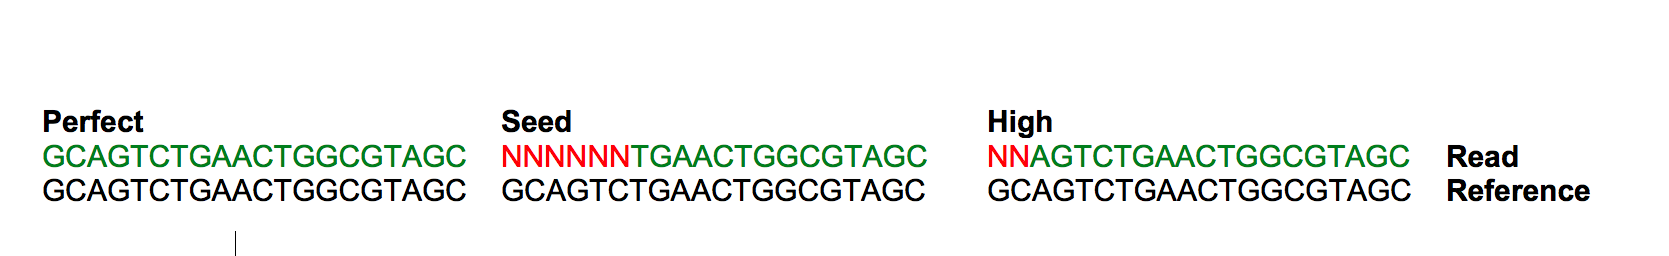
\includegraphics{./pictures/alignment-match.png}

\paragraph{Example of a MIACCS File entry for FASTQ
files}\label{example-of-a-miaccs-file-entry-for-fastq-files}

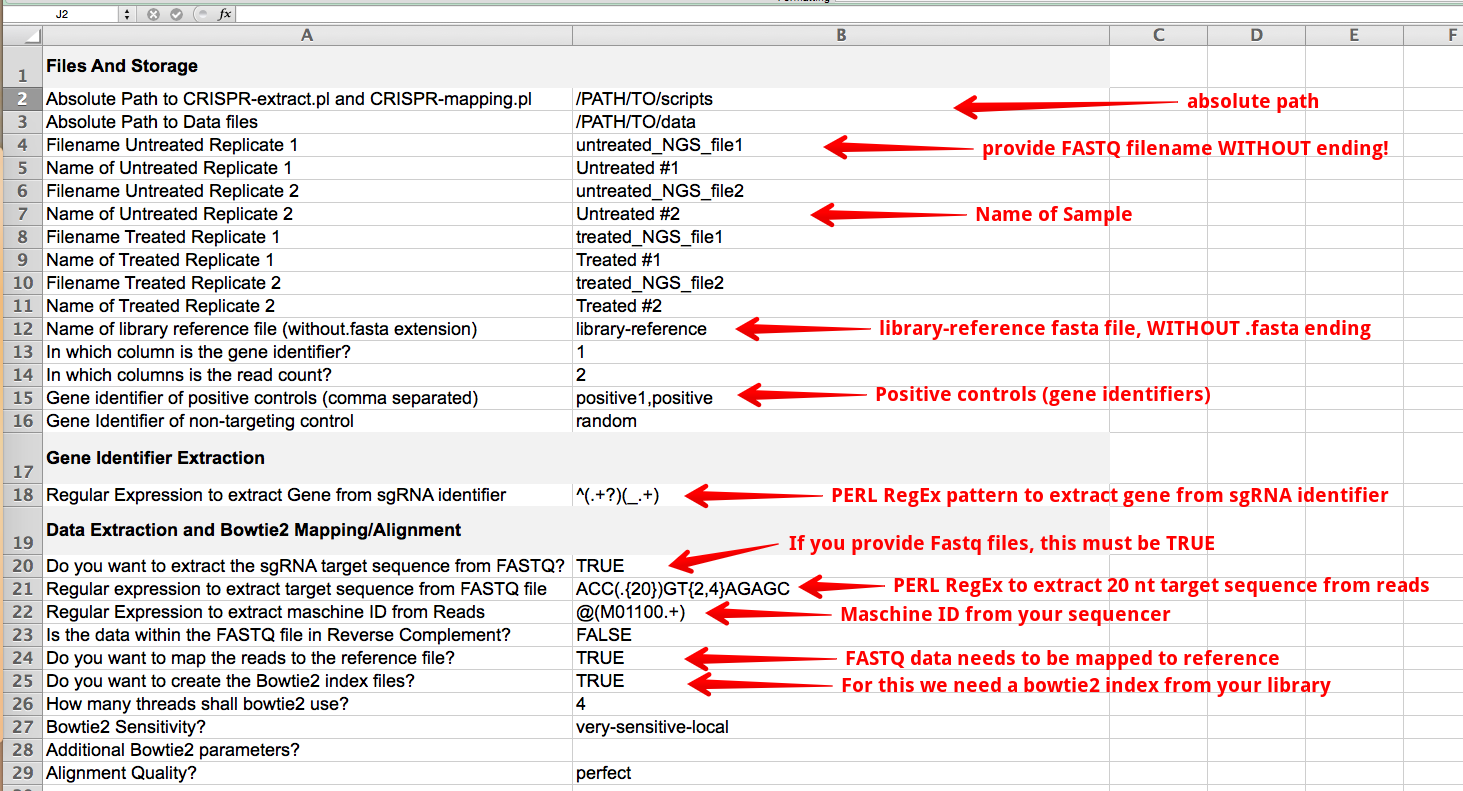
\includegraphics{./pictures/miaccs-fastq.png}

\subsubsection{Using Read Count Files}\label{using-read-count-files}

Instead of using raw NGS Fastq files, caRpools can also be used to
directly analysis read-count files without fastq data extraction and
mapping.\\
In this case, already finalized read-count files are provided that must
be in the same format as described in \textbf{Read Count Data Files}.

If you provide read-count files, please make sure you fill out the
MIACCS file accordingly.\\
An example of a MIACCS file for read-count files is shown below.

\paragraph{Example of a MIACCS File entry for Read-Count
files}\label{example-of-a-miaccs-file-entry-for-read-count-files}

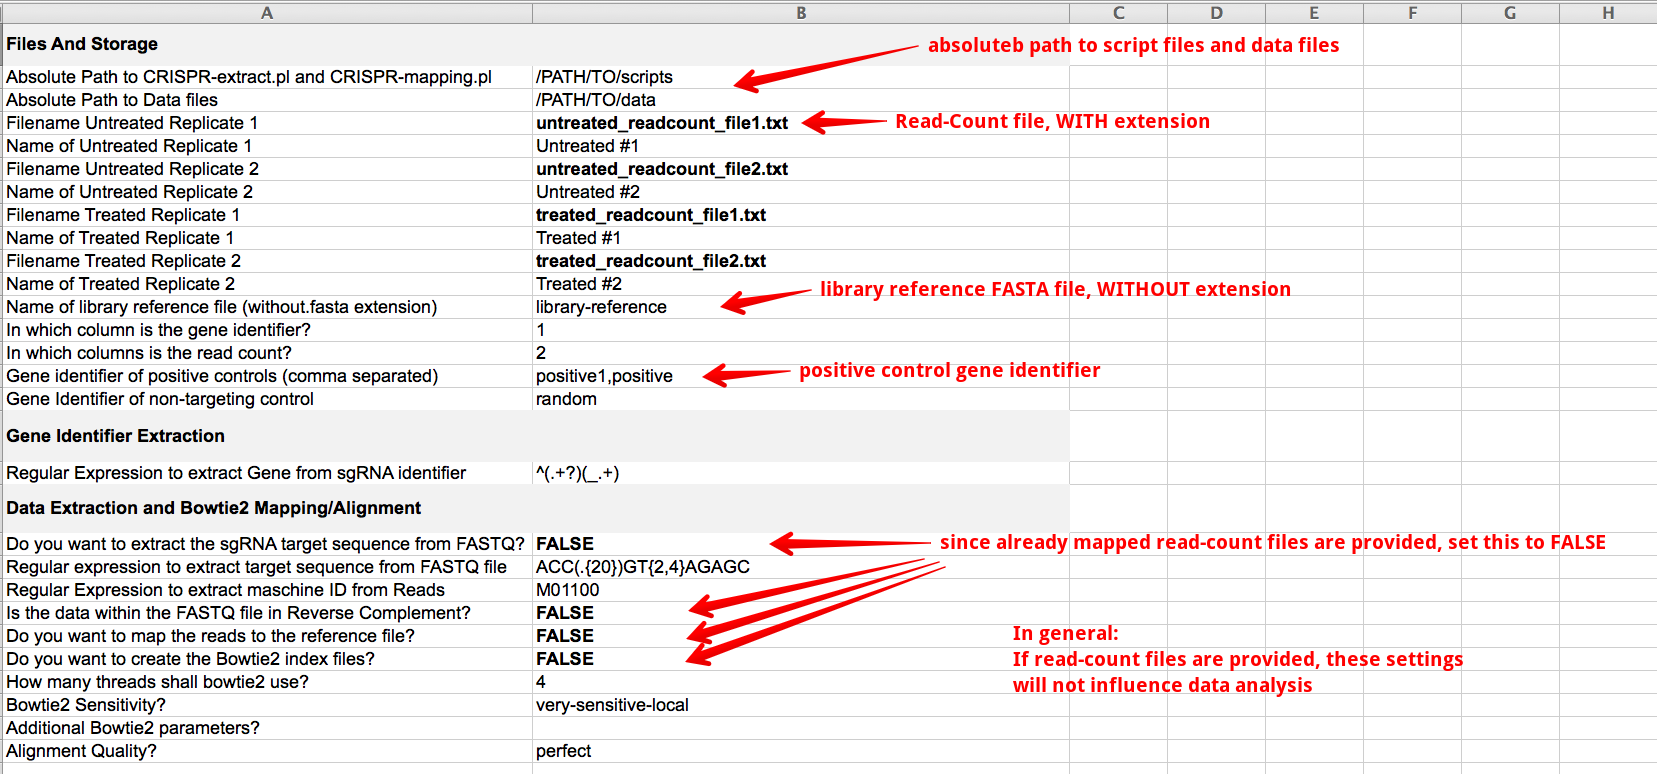
\includegraphics{./pictures/miaccs-readcount.png}

\subsubsection{Data Analysis Options}\label{data-analysis-options}

CaRpools is not only meant as a tool for standardized and fully
reproducible data analysis of CRISPR-Cas screens, but also fosters
exploratory data analysis.\\
Therefore caRpools offers the user different options for data analsysis
as illustrated below. All options can be set within the MIACCS file or
directly passed on to the individual functions of caRpools (advanced
users).

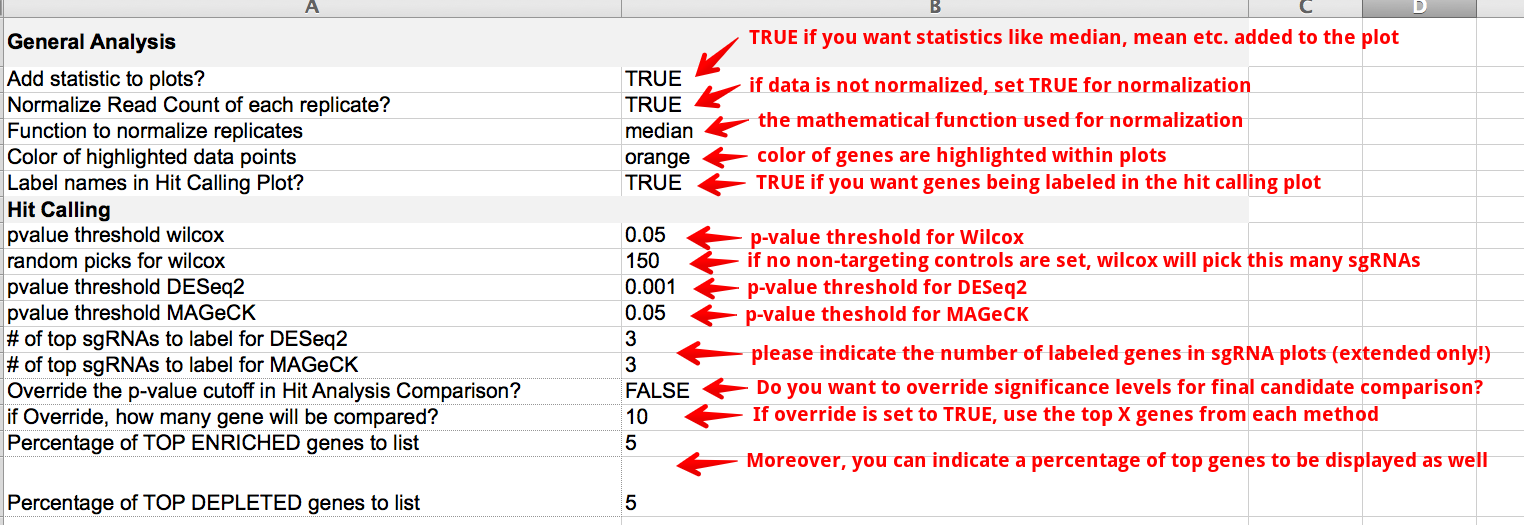
\includegraphics{./pictures/miaccs-analysis.png}

\section{Start CaRpools Report
Generation}\label{start-carpools-report-generation}

You can start caRpools Report Generation after you did the following
steps:

\begin{itemize}
\tightlist
\item
  Installed all required software and R packages (use
  \emph{check.caRpools(files=FALSE)} to verify)
\item
  Put every file in the correct folder (MIACCS, data files, script
  files, Rmd templates)
\item
  Put everythin in the R working directory or set the working directory
  to the folder of your files
\item
  Filled out the MIACCS file with all information, e.g.~correct
  filenames, reference, data analysis options
\end{itemize}

You can check for all requirements by calling \texttt{check.caRpools}.

\subsection{Start CaRpools using
R-Studio}\label{start-carpools-using-r-studio}

In the case you use R-Studio, you can start caRpools by just opening the
corresponding Rmd template file.\\
At the top, you will find the \textbf{Knit PDF} or \textbf{Knit HTML}
button, so you just need to press that and caRpools will generate the
report.

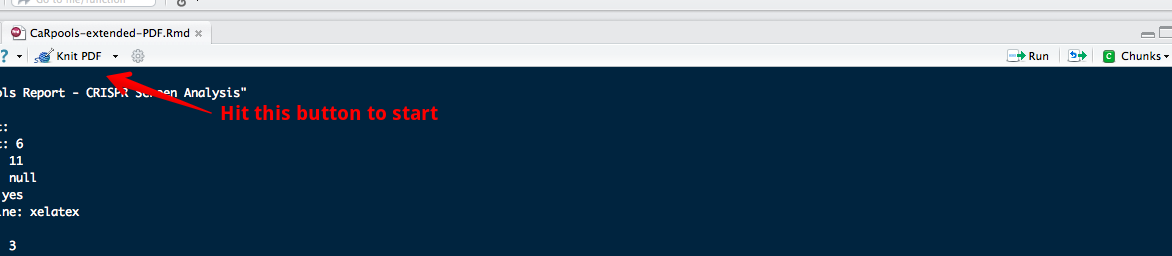
\includegraphics{./pictures/rstudio-knit.png}

As an alternative, you can start caRpools via \texttt{use.caRpools} and
provide additional parameters (see below).

\subsection{Start CaRpools using R
console}\label{start-carpools-using-r-console}

Moreover, caRpools report generation can also be initiated without
R-studio installation, so that this can be done via R command line even
on remote computers.\\
In this case, caRpools report generation can be started via
\texttt{use.caRpools} with additional parameters, which are described
below.

\paragraph{use.caRpools()}\label{use.carpools}

\textbf{Usage:}\\
\texttt{use.caRpools(type=NULL,\ file="CaRpools-extended-PDF.Rmd",\ miaccs="MIACCS.xls",\ check=TRUE,\ work.dir=NULL)}

\textbf{type}\\
\emph{Description} If you provide a custom Rmd template that can
generate both, PDF and HTML reports you can indicate which version you
want to generate.\\
\emph{Default} NULL\\
\emph{Values} ``PDF'', ``HTML''

\textbf{file}\\
\emph{Description} The file name of your custom Rmd template file (with
extension).\\
\emph{Default} ``CaRpools-extended-PDF.Rmd''\\
\emph{Values} filename as character

\textbf{miaccs}\\
\emph{Description} The filename of your MIACCS file.\\
\emph{Default} ``MIACCS.xls''\\
\emph{Values} filename as character

\textbf{check}\\
\emph{Description} Indicates whether caRpools will check for correct
installation and file access.\\
\emph{Default} TRUE\\
\emph{Values} TRUE or FALSE (boolean)

\textbf{work.dir}\\
\emph{Description} You can provide the absolute path to the working
directory in which all files are placed (e.g.~the MIACCS.xls and Rmd
template).\\
\emph{Default} NULL \emph{Values} absolute path (character) or NULL if
standard R working directory is used

\newpage

\section{Using CaRpools as a stand-alone R
Package}\label{using-carpools-as-a-stand-alone-r-package}

\textbf{CaRpools can be used without the provided R markdown templates
to generate own reports or individualized analysis of CRISPR/Cas9
screens.}\\
The following sections will explain every function included in CaRpools
and provide hints, tips and a documentation of how to use CaRpools for
data analysis. This will help you in customizing the generated reports
to you needs, create new reports or just use single functions of
CaRpools within your data analysis workflow.

\subsection{Loading Data}\label{loading-data}

CaRpools offers two ways of providing CRISPR/Cas9 screening data.\\
Either raw \textbf{read-count files} are directly used as described
before, or read-count files are generated from NGS FASTQ files by
extracting the 20 nt target sequence, mapping it against a reference
library and extracting the read-count information for each sgRNA
identifier.

\begin{Shaded}
\begin{Highlighting}[]
\NormalTok{CONTROL1 =}\StringTok{ }\KeywordTok{load.file}\NormalTok{(}\StringTok{"./data/untreated1.txt"}\NormalTok{, }\DataTypeTok{header=} \OtherTok{TRUE}\NormalTok{, }\DataTypeTok{sep=}\StringTok{"}\CharTok{\textbackslash{}t}\StringTok{"}\NormalTok{)}
\end{Highlighting}
\end{Shaded}

\textbf{Usage}\\
\texttt{load.file(filename,\ header\ =\ TRUE,\ sep="\textbackslash{}t",\ comment.char="",\ type\ =\ NULL)}

\textbf{filename} Filename to be loaded. If read-count files are loaded,
please include the extension. For FASTQ files, please pass on the output
of \texttt{data.extract} as this is the filename of the extracted
file.\\
\emph{Default} empty\\
\emph{Values} filename (character) or output from \texttt{data.extract}

\textbf{header}\\
Is the first line just a header?\\
\emph{Default} TRUE\\
\emph{Values} TRUE, FALSE (boolean)

\textbf{sep}\\
Seperator of data, usually tab-separated.\\
\emph{Default} ``\t'' for TAB-separated data\\
\emph{Values} Any separator

\textbf{comment.char}\\
Are character files within any quote etc? \emph{Default} ``''
\emph{Values} Any character

\textbf{type}\\
Indicates which files are being loaded. Three filetypes are possible.
Either NULL for tab-separated files, fastalib for library reference
files or xlsx for loading the MIACCS file.\\
\emph{Default} NULL \emph{Values} NULL, ``fastalib'', ``xlsx''

\subsubsection{Loading Read-Count files
Directly}\label{loading-read-count-files-directly}

Read-Count files (normalized or not normalized) can be loaded with
\texttt{load.file} into a data frame that is used for further usage.\\
For each untreated and treated sample two replicates are used:

\begin{Shaded}
\begin{Highlighting}[]
\NormalTok{CONTROL1 =}\StringTok{ }\KeywordTok{load.file}\NormalTok{(}\StringTok{"./data/untreated1.txt"}\NormalTok{, }\DataTypeTok{header=} \OtherTok{TRUE}\NormalTok{, }\DataTypeTok{sep=}\StringTok{"}\CharTok{\textbackslash{}t}\StringTok{"}\NormalTok{)}
\NormalTok{CONTROL =}\StringTok{ }\KeywordTok{load.file}\NormalTok{(}\StringTok{"./data/untreated2.txt"}\NormalTok{, }\DataTypeTok{header=} \OtherTok{TRUE}\NormalTok{, }\DataTypeTok{sep=}\StringTok{"}\CharTok{\textbackslash{}t}\StringTok{"}\NormalTok{)}
\NormalTok{TREAT1 =}\StringTok{ }\KeywordTok{load.file}\NormalTok{(}\StringTok{"./data/treated1.txt"}\NormalTok{, }\DataTypeTok{header=} \OtherTok{TRUE}\NormalTok{, }\DataTypeTok{sep=}\StringTok{"}\CharTok{\textbackslash{}t}\StringTok{"}\NormalTok{)}
\NormalTok{TREAT2 =}\StringTok{ }\KeywordTok{load.file}\NormalTok{(}\StringTok{"./data/treated2.txt"}\NormalTok{, }\DataTypeTok{header=} \OtherTok{TRUE}\NormalTok{, }\DataTypeTok{sep=}\StringTok{"}\CharTok{\textbackslash{}t}\StringTok{"}\NormalTok{)}

\CommentTok{# Don't forget the library reference}
\NormalTok{libFILE =}\StringTok{ }\KeywordTok{load.file}\NormalTok{(}
  \KeywordTok{paste}\NormalTok{(datapath, }\KeywordTok{paste}\NormalTok{(referencefile,}\StringTok{".fasta"}\NormalTok{,}\DataTypeTok{sep=}\StringTok{""}\NormalTok{), }\DataTypeTok{sep=}\StringTok{"/"}\NormalTok{),}\DataTypeTok{header =} \OtherTok{FALSE}\NormalTok{,}
  \DataTypeTok{type=}\StringTok{"fastalib"}\NormalTok{)}
\end{Highlighting}
\end{Shaded}

\subsubsection{Loading FASTQ Files to Generate Read-Count
Files}\label{loading-fastq-files-to-generate-read-count-files}

In a first step, NGS FASTQ data is extracted and mapped against a
reference library file using bowtie2.

\begin{Shaded}
\begin{Highlighting}[]
\NormalTok{fileCONTROL1 =}\StringTok{ }\KeywordTok{data.extract}\NormalTok{(}
  \DataTypeTok{scriptpath=}\StringTok{"path.to.scripts"}\NormalTok{, }\DataTypeTok{datapath=}\StringTok{"path.to.FASTQ"}\NormalTok{,}\DataTypeTok{fastqfile=}\StringTok{"filename1"}\NormalTok{,}
  \DataTypeTok{extract=}\OtherTok{TRUE}\NormalTok{, seq.pattern, maschine.pattern, }\DataTypeTok{createindex=}\OtherTok{TRUE}\NormalTok{,}
  \DataTypeTok{bowtie2file=}\NormalTok{filename.lib.reference, }\DataTypeTok{referencefile=}\StringTok{"filename.lib.reference"}\NormalTok{,}
  \DataTypeTok{mapping=}\OtherTok{TRUE}\NormalTok{, }\DataTypeTok{reversecomplement=}\OtherTok{FALSE}\NormalTok{, threads, bowtieparams,}
  \DataTypeTok{sensitivity=}\StringTok{"very-sensitive-local"}\NormalTok{,}\DataTypeTok{match=}\StringTok{"perfect"}\NormalTok{)  }
\CommentTok{# Now we can load the generated Read-Count file directly!}
\NormalTok{CONTROL1 =}\StringTok{ }\KeywordTok{load.file}\NormalTok{(}\KeywordTok{paste}\NormalTok{(datapath, fileCONTROL1, }\DataTypeTok{sep=}\StringTok{"/"}\NormalTok{)) }\CommentTok{# Untreated sample 1 loaded}

\CommentTok{# Don't forget the library reference}
\NormalTok{libFILE =}\StringTok{ }\KeywordTok{load.file}\NormalTok{(}
  \KeywordTok{paste}\NormalTok{(datapath, }\KeywordTok{paste}\NormalTok{(referencefile,}\StringTok{".fasta"}\NormalTok{,}\DataTypeTok{sep=}\StringTok{""}\NormalTok{), }\DataTypeTok{sep=}\StringTok{"/"}\NormalTok{),}\DataTypeTok{header =} \OtherTok{FALSE}\NormalTok{,}
  \DataTypeTok{type=}\StringTok{"fastalib"}\NormalTok{)}
\end{Highlighting}
\end{Shaded}

A closer look to the data frame we just loaded:

\begin{longtable}[c]{@{}llr@{}}
\toprule
& sgRNA & Count\tabularnewline
\midrule
\endhead
40 & ABI1\_129\_0 & 12\tabularnewline
41 & ABI1\_12\_0 & 50\tabularnewline
42 & ABI1\_132\_0 & 131\tabularnewline
43 & ABI1\_132\_16356 & 90\tabularnewline
44 & ABI1\_132\_65424 & 28\tabularnewline
45 & ABI1\_133\_0 & 14\tabularnewline
46 & ABI1\_134\_0 & 49\tabularnewline
47 & ABI1\_134\_49068 & 92\tabularnewline
48 & ABL1\_0\_148908 & 146\tabularnewline
49 & ABL1\_108\_148908 & 126\tabularnewline
50 & ABL1\_109\_148908 & 62\tabularnewline
\bottomrule
\end{longtable}

\paragraph{data.extract()}\label{data.extract}

\textbf{Usage:}\\
\texttt{data.extract(scriptpath=NULL,\ datapath=NULL,\ fastqfile=NULL,\ extract\ =\ FALSE,\ pattern\ =\ "default",\ maschinepattern\ =\ "default",\ createindex\ =\ FALSE,\ bowtie2file\ =\ NULL,\ referencefile=\ NULL,\ mapping\ =\ FALSE,\ reversecomplement\ =\ FALSE,\ threads\ =\ 1,\ bowtieparams\ =\ "",\ sensitivity\ =\ "very-sensitive-local",\ match\ =\ "perfect")}

\textbf{scriptpath}\\
Absolute path of the folder that contains \texttt{CRISPR-extract.pl} and
\texttt{CRISPR-mapping.pl}\\
\emph{Default} NULL\\
\emph{Values} absolute path (character)

\textbf{datapath}\\
Absolute path of the folder that contains the data files
(e.g.~file.FASTQ)\\
\emph{Default} NULL\\
\emph{Values} absolute path (character)

\textbf{fastqfile}\\
Filename of FASTQ file WITHOUT .fastq extension\\
\emph{Default} NULL\\
\emph{Values} filename (character)

\textbf{extract}\\
Whether CRISPR-extract.pl is used to extract the 20 nt target sequence
from the NGS reads using \texttt{pattern} \emph{Default} FALSE\\
\emph{Values} TRUE, FALSE (boolean)

\textbf{pattern}\\
PERL regular Expression to extract 20 nt target sequence from NGS reads.
Please see \emph{extract pattern} in this manual for more information.\\
\emph{Default} Regular Expression (character)

\subsubsection{Aggregating sgRNA read-count to Gene
read-count}\label{aggregating-sgrna-read-count-to-gene-read-count}

CaRpools allows you to aggregate sgRNA read-counts to gene read-counts
using \texttt{aggregatetogenes()}.

\begin{Shaded}
\begin{Highlighting}[]
\NormalTok{CONTROL1.g=}\KeywordTok{aggregatetogenes}\NormalTok{(}\DataTypeTok{data.frame =} \NormalTok{CONTROL1, }\DataTypeTok{agg.function=}\NormalTok{sum,}
                            \DataTypeTok{extractpattern =} \KeywordTok{expression}\NormalTok{(}\StringTok{"^(.+?)(_.+)"}\NormalTok{))}
\end{Highlighting}
\end{Shaded}

\paragraph{aggregatetogenes()}\label{aggregatetogenes}

\textbf{Usage}\\
\texttt{aggregatetogenes(data.frame,\ namecolumn=1,\ countcolumn=2,\ agg.function=sum,\ extractpattern=expression("\^{}(.+?)\_.+"),\ type="aggregate")}

\textbf{data.frame}\\
A data-frame of sgRNA read-count data as done by \texttt{load.file}\\
\emph{Default} empty\\
\emph{Values} data-frame

\textbf{namecolumn}\\
In which column are the sgRNA identifiers?\\
\emph{Default} 1\\
\emph{Values} column number (numeric)

\textbf{countcolumn}\\
In which column are the read counts?\\
\emph{Default} 2\\
\emph{Values} column number (numeric)

\textbf{extractpattern}\\
PERL regular expression that is used to retrieve the gene identifier
from the overall sgRNA identifier.\\
e.g.~in \textbf{AAK1\_107\_0} it will extract \textbf{AAK1}, since this
is the gene identifier beloning to this sgRNA identifier. \textbf{Please
see: Read-Count Data Files}\\
\emph{Default} expression(``\^{}(.+?)(\_.+)``), will work for most
available libraries.\\
\emph{Values} PERL regular expression with parenthesis indicating the
gene identifier (expression)

\textbf{type}\\
CaRpools can either aggregate the data frame
(\texttt{type\ =\ "annotate"}) or annotate the gene identifiers only as
an additional column (\texttt{type\ =\ "annotate"}).\\
\emph{Default} ``aggregate''\\
\emph{Values} ``aggregate'', ``annotate''

\subparagraph{Example for data
aggregation}\label{example-for-data-aggregation}

\begin{Shaded}
\begin{Highlighting}[]
\NormalTok{CONTROL1.g=}\KeywordTok{aggregatetogenes}\NormalTok{(}\DataTypeTok{data.frame =} \NormalTok{CONTROL1, }\DataTypeTok{agg.function=}\NormalTok{sum,}
            \DataTypeTok{extractpattern =} \KeywordTok{expression}\NormalTok{(}\StringTok{"^(.+?)(_.+)"}\NormalTok{), }\DataTypeTok{type=}\StringTok{"aggregate"}\NormalTok{)}
\NormalTok{knitr::}\KeywordTok{kable}\NormalTok{(CONTROL1.g[}\DecValTok{1}\NormalTok{:}\DecValTok{10}\NormalTok{,])}
\end{Highlighting}
\end{Shaded}

\begin{longtable}[c]{@{}llrl@{}}
\toprule
& sgRNA & Count & Gene\tabularnewline
\midrule
\endhead
AAK1 & AAK1 & 881 & AAK1\tabularnewline
AATK & AATK & 2114 & AATK\tabularnewline
ABI1 & ABI1 & 1591 & ABI1\tabularnewline
ABL1 & ABL1 & 1015 & ABL1\tabularnewline
ABL2 & ABL2 & 1257 & ABL2\tabularnewline
ACAD10 & ACAD10 & 968 & ACAD10\tabularnewline
ACVR1 & ACVR1 & 1526 & ACVR1\tabularnewline
ACVR1B & ACVR1B & 1109 & ACVR1B\tabularnewline
ACVR1C & ACVR1C & 1248 & ACVR1C\tabularnewline
ACVR2A & ACVR2A & 749 & ACVR2A\tabularnewline
\bottomrule
\end{longtable}

\subparagraph{Example for data
annotation}\label{example-for-data-annotation}

\begin{Shaded}
\begin{Highlighting}[]
\NormalTok{CONTROL1.g.annotate=}\KeywordTok{aggregatetogenes}\NormalTok{(}\DataTypeTok{data.frame =} \NormalTok{CONTROL1, }\DataTypeTok{agg.function=}\NormalTok{sum,}
            \DataTypeTok{extractpattern =} \KeywordTok{expression}\NormalTok{(}\StringTok{"^(.+?)(_.+)"}\NormalTok{), }\DataTypeTok{type=}\StringTok{"annotate"}\NormalTok{)}
\NormalTok{knitr::}\KeywordTok{kable}\NormalTok{(CONTROL1.g.annotate[}\DecValTok{1}\NormalTok{:}\DecValTok{10}\NormalTok{,])}
\end{Highlighting}
\end{Shaded}

\begin{longtable}[c]{@{}lrl@{}}
\toprule
sgRNA & Count & Gene\tabularnewline
\midrule
\endhead
AAK1\_104\_0 & 0 & AAK1\tabularnewline
AAK1\_105\_0 & 197 & AAK1\tabularnewline
AAK1\_106\_0 & 271 & AAK1\tabularnewline
AAK1\_107\_0 & 1 & AAK1\tabularnewline
AAK1\_108\_0 & 0 & AAK1\tabularnewline
AAK1\_109\_0 & 89 & AAK1\tabularnewline
AAK1\_111\_182532 & 0 & AAK1\tabularnewline
AAK1\_111\_60844 & 11 & AAK1\tabularnewline
AAK1\_112\_60844 & 55 & AAK1\tabularnewline
AAK1\_113\_60844 & 16 & AAK1\tabularnewline
\bottomrule
\end{longtable}

\subsubsection{Convert Gene Identifier or Annotate Gene
Information}\label{convert-gene-identifier-or-annotate-gene-information}

It is also possible to either enrich the screening dataset file with
additional information provided by the biomaRt interface.\\
For example, gene identifiers can be changed from EnsemblIDs to official
gene symbols are Gene Ontology terms can be added to the dataset.\\
This can be done using \texttt{get.gene.info}, which serves as a wrapper
for the \textbf{biomaRt} package with its load of options and
possibilities (more information see \texttt{?biomaRt}).

You can convert any gene identifier which is included in your sgRNA
identifer to e.g.~EnsemblID or HGNC Gene Symbol using caRpools.\\
\textbf{Please note that Internet Access is required for biomaRt.}\\
For further information about biomaRt conversion, please see the
\href{www.bioconductor.org/packages/release/bioc/vignettes/biomaRt/inst/doc/biomaRt.pdf}{biomaRt
Manual}.

\begin{Shaded}
\begin{Highlighting}[]
\CommentTok{# Convert HGNC gene symbol to EnsemblID}
\NormalTok{CONTROL1 =}\StringTok{ }\KeywordTok{get.gene.info}\NormalTok{(}
  \NormalTok{CONTROL1, }\DataTypeTok{namecolumn=}\DecValTok{1}\NormalTok{, }\DataTypeTok{extractpattern=}\KeywordTok{expression}\NormalTok{(}\StringTok{"^(.+?)(_.+)"}\NormalTok{),}
  \DataTypeTok{database=}\StringTok{"ensembl"}\NormalTok{, }\DataTypeTok{dataset=}\StringTok{"hsapiens_gene_ensembl"}\NormalTok{, }\DataTypeTok{filters=}\StringTok{"hgnc_symbol"}\NormalTok{,}
  \DataTypeTok{attributes =} \StringTok{"ensembl_gene_id"}\NormalTok{, }\DataTypeTok{return.val =} \StringTok{"dataset"}\NormalTok{)}
\CommentTok{# Also convert the library reference}
\NormalTok{libFILE =}\StringTok{ }\KeywordTok{get.gene.info}\NormalTok{(}
  \NormalTok{libFILE, }\DataTypeTok{namecolumn=}\DecValTok{1}\NormalTok{, }\DataTypeTok{extractpattern=}\KeywordTok{expression}\NormalTok{(}\StringTok{"^(.+?)(_.+)"}\NormalTok{),}
  \DataTypeTok{database=}\StringTok{"ensembl"}\NormalTok{, }\DataTypeTok{dataset=}\StringTok{"hsapiens_gene_ensembl"}\NormalTok{, }\DataTypeTok{filters=}\StringTok{"hgnc_symbol"}\NormalTok{,}
  \DataTypeTok{attributes =} \StringTok{"ensembl_gene_id"}\NormalTok{, }\DataTypeTok{return.val =} \StringTok{"dataset"}\NormalTok{)}
\end{Highlighting}
\end{Shaded}

This will convert a gene identifier, which is extracted by a PERL
Regular Expression **(.+?)(\_.+)** and of type hgnc\_symbol (gene
symbol), to an Ensembl Gene ID.

\paragraph{get.gene.info()}\label{get.gene.info}

\textbf{Usage}\\
\texttt{get.gene.info\ =\ function(data,\ namecolumn=1,\ extractpattern=expression("\^{}(.+?)(\_.+)"),\ database="ensembl",\ dataset="hsapiens\_gene\_ensembl",\ filters="ensembl\_gene\_id",\ attributes\ =\ c("hgnc\_symbol"),\ return.val\ =\ "dataset",\ controls=FALSE)}

\textbf{data} Data frame that contains read-count data. \emph{Default}
none \emph{Values} data.frame containing read-count data (data.frame)

\textbf{namecolumn}\\
In which column are the sgRNA identifiers?\\
\emph{Default} 1\\
\emph{Values} column number (numeric)

\textbf{extractpattern}\\
PERL regular expression that is used to retrieve the gene identifier
from the overall sgRNA identifier.\\
e.g.~in \textbf{AAK1\_107\_0} it will extract \textbf{AAK1}, since this
is the gene identifier beloning to this sgRNA identifier. \textbf{Please
see: Read-Count Data Files}\\
\emph{Default} expression(``\^{}(.+?)(\_.+)``), will work for most
available libraries.\\
\emph{Values} PERL regular expression with parenthesis indicating the
gene identifier (expression)

\textbf{database}\\
BiomaRt database to be used. See \texttt{?listMarts()} or biomaRt
documentation.\\
\emph{Default} ``ensembl'', is using the ensembl database\\
\emph{Values} Any biomaRt database (character)

\textbf{dataset}\\
The biomaRt dataset to be used. For \emph{homo sapiens},
\emph{hsapiens\_gene\_ensembl} is recommended. See
\texttt{?listDatasets} or biomaRt documentation.\\
\emph{Default} ``hsapiens\_gene\_ensembl''\\
\emph{Values} Any biomaRt dataset (character)

\textbf{filters}\\
The input filter information to retrieve biomaRt annotation, usually is
the type of gene identifier used in the read-count files, e.g.
``ensemble\_gene\_id''. see \texttt{?listFilters}\\
\emph{Default} ``ensembl\_gene\_id''\\
\emph{Values} Any biomaRt filter (character)

\textbf{attributes}\\
The output attribute to retrieve from biomaRt, usually the annotations
that need to be fetched, e.g. ``hgnc\_symbol''. see
\texttt{?listAttributes}\\
\emph{Default} ``hgnc\_symbol''\\
\emph{Values} Any biomaRt attribute (character)

\textbf{return.val}\\
The type of object that is returned. For whole dataset, e.g.~conversion
of gene identifiers, use ``dataset''.\\
\emph{Default} ``dataset''\\
\emph{Values} ``dataset'' (will give back the same data frame, but with
exchanged gene identifiers), ``info'' (will return a data frame with all
attributes fetched for genes, is used to annotate gene with additional
information)

\textbf{controls}\\
Is set to TRUE if \texttt{data} is not a data frame, but a vector.\\
\emph{Default} FALSE\\
\emph{Values} TRUE, FALSE (boolean)

\subparagraph{Example: Replace Gene Identifier (EnsemblID) by Official
Gene
Symbol}\label{example-replace-gene-identifier-ensemblid-by-official-gene-symbol}

\begin{Shaded}
\begin{Highlighting}[]
\NormalTok{CONTROL1.replaced =}\StringTok{ }\KeywordTok{get.gene.info}\NormalTok{(CONTROL1, }\DataTypeTok{namecolumn=}\DecValTok{1}\NormalTok{,}
      \DataTypeTok{extractpattern=}\KeywordTok{expression}\NormalTok{(}\StringTok{"^(.+?)(_.+)"}\NormalTok{), }\DataTypeTok{database=}\StringTok{"ensembl"}\NormalTok{, }\DataTypeTok{dataset=}\StringTok{"hsapiens_gene_ensembl"}\NormalTok{,}
      \DataTypeTok{filters=}\StringTok{"hgnc_symbol"}\NormalTok{, }\DataTypeTok{attributes =} \KeywordTok{c}\NormalTok{(}\StringTok{"ensembl_gene_id"}\NormalTok{), }\DataTypeTok{return.val =} \StringTok{"dataset"}\NormalTok{)}

\NormalTok{knitr::}\KeywordTok{kable}\NormalTok{(CONTROL1.replaced[}\DecValTok{1}\NormalTok{:}\DecValTok{10}\NormalTok{,])}
\end{Highlighting}
\end{Shaded}

\begin{longtable}[c]{@{}lr@{}}
\toprule
sgRNA & Count\tabularnewline
\midrule
\endhead
ENSG00000115977\_104\_0 & 0\tabularnewline
ENSG00000115977\_105\_0 & 197\tabularnewline
ENSG00000115977\_106\_0 & 271\tabularnewline
ENSG00000115977\_107\_0 & 1\tabularnewline
ENSG00000115977\_108\_0 & 0\tabularnewline
ENSG00000115977\_109\_0 & 89\tabularnewline
ENSG00000115977\_111\_182532 & 0\tabularnewline
ENSG00000115977\_111\_60844 & 11\tabularnewline
ENSG00000115977\_112\_60844 & 55\tabularnewline
ENSG00000115977\_113\_60844 & 16\tabularnewline
\bottomrule
\end{longtable}

\subparagraph{Example: Enrich Dataset by Gene
Description}\label{example-enrich-dataset-by-gene-description}

\begin{Shaded}
\begin{Highlighting}[]
\NormalTok{CONTROL1.replaced.info =}\StringTok{ }\KeywordTok{get.gene.info}\NormalTok{(CONTROL1, }\DataTypeTok{namecolumn=}\DecValTok{1}\NormalTok{,}
      \DataTypeTok{extractpattern=}\KeywordTok{expression}\NormalTok{(}\StringTok{"^(.+?)(_.+)"}\NormalTok{), }\DataTypeTok{database=}\StringTok{"ensembl"}\NormalTok{, }\DataTypeTok{dataset=}\StringTok{"hsapiens_gene_ensembl"}\NormalTok{,}
      \DataTypeTok{filters=}\StringTok{"hgnc_symbol"}\NormalTok{, }\DataTypeTok{attributes =} \KeywordTok{c}\NormalTok{(}\StringTok{"ensembl_gene_id"}\NormalTok{,}\StringTok{"description"}\NormalTok{), }\DataTypeTok{return.val =} \StringTok{"info"}\NormalTok{)}

\NormalTok{knitr::}\KeywordTok{kable}\NormalTok{(CONTROL1.replaced.info[}\DecValTok{1}\NormalTok{:}\DecValTok{10}\NormalTok{,])}
\end{Highlighting}
\end{Shaded}

\begin{longtable}[c]{@{}lll@{}}
\toprule
hgnc\_symbol & ensembl\_gene\_id & description\tabularnewline
\midrule
\endhead
AAK1 & ENSG00000115977 & AP2 associated kinase 1 {[}Source:HGNC
Symbol;Acc:HGNC:19679{]}\tabularnewline
AATK & ENSG00000181409 & apoptosis-associated tyrosine kinase
{[}Source:HGNC Symbol;Acc:HGNC:21{]}\tabularnewline
ABI1 & ENSG00000136754 & abl-interactor 1 {[}Source:HGNC
Symbol;Acc:HGNC:11320{]}\tabularnewline
ABL1 & ENSG00000097007 & ABL proto-oncogene 1, non-receptor tyrosine
kinase {[}Source:HGNC Symbol;Acc:HGNC:76{]}\tabularnewline
ABL2 & ENSG00000143322 & ABL proto-oncogene 2, non-receptor tyrosine
kinase {[}Source:HGNC Symbol;Acc:HGNC:77{]}\tabularnewline
ACAD10 & ENSG00000111271 & acyl-CoA dehydrogenase family, member 10
{[}Source:HGNC Symbol;Acc:HGNC:21597{]}\tabularnewline
ACVR1 & ENSG00000115170 & activin A receptor, type I {[}Source:HGNC
Symbol;Acc:HGNC:171{]}\tabularnewline
ACVR1B & ENSG00000135503 & activin A receptor, type IB {[}Source:HGNC
Symbol;Acc:HGNC:172{]}\tabularnewline
ACVR1C & ENSG00000123612 & activin A receptor, type IC {[}Source:HGNC
Symbol;Acc:HGNC:18123{]}\tabularnewline
ACVR2A & ENSG00000121989 & activin A receptor, type IIA {[}Source:HGNC
Symbol;Acc:HGNC:173{]}\tabularnewline
\bottomrule
\end{longtable}

\newpage

\subsection{Quality Control of pooled CRISPR Screening
data}\label{quality-control-of-pooled-crispr-screening-data}

There are several different functions available to determine the quality
of your data:

\begin{itemize}
\tightlist
\item
  General Dataset Statistics
\item
  Specific Statistics of Included Controls
\item
  Readcount Distribution \texttt{plot.read.distribution}
\item
  Read Depth \texttt{plot.read.depth}
\item
  sgRNAs present per Gene Target \texttt{plot.reads.genedesigns}
\item
  Readcount comparison of different samples \texttt{plot.read.count.vs}
\item
  Information about the phenotype of sgRNAs \texttt{plot.raw.genes}
\end{itemize}

\subsubsection{Dataset Statistics}\label{dataset-statistics}

General statistics for a given dataset can be obtained by
\texttt{stats.data}.\\
For further information about the possibilities, see
\texttt{?stats.data}.

A typical table would look like this (shorted):

\begin{longtable}[c]{@{}lrrrr@{}}
\toprule
Readcount & Control \#1 & Control \#2 & TRAIL \#1 & TRAIL
\#2\tabularnewline
\midrule
\endhead
Mean & 79 & 108 & 109 & 109\tabularnewline
Median & 51 & 74 & 41 & 39\tabularnewline
SD & 90 & 115 & 244 & 260\tabularnewline
Min & 0 & 0 & 0 & 0\tabularnewline
Max & 1141 & 1304 & 6819 & 8257\tabularnewline
\# sgRNA not present & 934 & 817 & 1563 & 1573\tabularnewline
\bottomrule
\end{longtable}

\begin{Shaded}
\begin{Highlighting}[]
\CommentTok{# General}
\NormalTok{U1.stats =}\StringTok{ }\KeywordTok{stats.data}\NormalTok{(}\DataTypeTok{dataset=}\NormalTok{CONTROL1, }\DataTypeTok{namecolumn =} \DecValTok{1}\NormalTok{, }\DataTypeTok{fullmatchcolumn =} \DecValTok{2}\NormalTok{,}
                      \DataTypeTok{extractpattern=}\KeywordTok{expression}\NormalTok{(}\StringTok{"^(.+?)_.+"}\NormalTok{), }\DataTypeTok{type=}\StringTok{"stats"}\NormalTok{)}
\NormalTok{U2.stats =}\StringTok{ }\KeywordTok{stats.data}\NormalTok{(}\DataTypeTok{dataset=}\NormalTok{CONTROL2, }\DataTypeTok{namecolumn =} \DecValTok{1}\NormalTok{, }\DataTypeTok{fullmatchcolumn =} \DecValTok{2}\NormalTok{,}
                      \DataTypeTok{extractpattern=}\KeywordTok{expression}\NormalTok{(}\StringTok{"^(.+?)_.+"}\NormalTok{), }\DataTypeTok{type=}\StringTok{"stats"}\NormalTok{)}
\NormalTok{T1.stats =}\KeywordTok{stats.data}\NormalTok{(}\DataTypeTok{dataset=}\NormalTok{TREAT1, }\DataTypeTok{namecolumn =} \DecValTok{1}\NormalTok{, }\DataTypeTok{fullmatchcolumn =} \DecValTok{2}\NormalTok{,}
                     \DataTypeTok{extractpattern=}\KeywordTok{expression}\NormalTok{(}\StringTok{"^(.+?)_.+"}\NormalTok{), }\DataTypeTok{type=}\StringTok{"stats"}\NormalTok{)}
\NormalTok{T2.stats =}\KeywordTok{stats.data}\NormalTok{(}\DataTypeTok{dataset=}\NormalTok{TREAT2, }\DataTypeTok{namecolumn =} \DecValTok{1}\NormalTok{, }\DataTypeTok{fullmatchcolumn =} \DecValTok{2}\NormalTok{,}
                     \DataTypeTok{extractpattern=}\KeywordTok{expression}\NormalTok{(}\StringTok{"^(.+?)_.+"}\NormalTok{), }\DataTypeTok{type=}\StringTok{"stats"}\NormalTok{)}
\CommentTok{# Combine Stats}
\NormalTok{combined.stats =}\StringTok{ }\KeywordTok{cbind.data.frame}\NormalTok{(U1.stats[,}\DecValTok{1}\NormalTok{:}\DecValTok{2}\NormalTok{], U2.stats[,}\DecValTok{2}\NormalTok{], T1.stats[,}\DecValTok{2}\NormalTok{], T2.stats[,}\DecValTok{2}\NormalTok{])}
\KeywordTok{colnames}\NormalTok{(combined.stats) =}\StringTok{ }\KeywordTok{c}\NormalTok{(}\StringTok{"Readcount"}\NormalTok{, d.CONTROL1, d.CONTROL2, d.TREAT1, d.TREAT2)}

\CommentTok{# output all to a file}
\NormalTok{xlsx::}\KeywordTok{write.xlsx}\NormalTok{(combined.stats, }\DataTypeTok{file=}\StringTok{"General-stats.xls"}\NormalTok{, }\DataTypeTok{sheetName=}\StringTok{"Combined Stats"}\NormalTok{, }\DataTypeTok{row.names=}\OtherTok{FALSE}\NormalTok{)}

\CommentTok{# Create stats for whole data set}
\NormalTok{U1.allstats =}\StringTok{ }\KeywordTok{stats.data}\NormalTok{(}\DataTypeTok{dataset=}\NormalTok{CONTROL1, }\DataTypeTok{namecolumn =} \NormalTok{namecolumn,}
    \DataTypeTok{fullmatchcolumn =} \NormalTok{fullmatchcolumn, }\DataTypeTok{extractpattern=}\NormalTok{g.extractpattern, }\DataTypeTok{type=}\StringTok{"dataset"}\NormalTok{)}
\end{Highlighting}
\end{Shaded}

\paragraph{stats.data()}\label{stats.data}

\textbf{Usage}\\
\texttt{stats.data\ =\ (dataset,\ namecolumn\ =\ 1,\ fullmatchcolumn\ =\ 2,\ extractpattern=expression("\^{}(.+?)\_.+"),\ readcount.unmapped.total\ =\ NA,\ controls.target\ =\ NULL,\ controls.nontarget\ =\ "random",\ type="stats")}

\textbf{dataset}\\
Data frame of read-count object.\\
\emph{Default} none\\
\emph{Values} data frame as created by \texttt{load.file()}

\textbf{namecolumn}\\
In which column are the sgRNA identifiers?\\
\emph{Default} 1\\
\emph{Values} column number (numeric)

\textbf{fullmatchcolumn}\\
In which column are the read counts?\\
\emph{Default} 2\\
\emph{Values} column number (numeric)

\textbf{extractpattern}\\
PERL regular expression that is used to retrieve the gene identifier
from the overall sgRNA identifier.\\
e.g.~in \textbf{AAK1\_107\_0} it will extract \textbf{AAK1}, since this
is the gene identifier beloning to this sgRNA identifier. \textbf{Please
see: Read-Count Data Files}\\
\emph{Default} expression(``\^{}(.+?)(\_.+)``), will work for most
available libraries.\\
\emph{Values} PERL regular expression with parenthesis indicating the
gene identifier (expression)

\textbf{readcount.unmapped.total}\\
Number of raw NGS reads, only used if \texttt{type="mapping}.\\
\emph{Default} NA\\
\emph{Values} Number of raw reads (integer)

\textbf{controls.target}\\
If \texttt{type="controls"}, this is the gene identifier of the positive
control.\\
\emph{Default} NULL\\
\emph{Value} Gene Identifier (character)

\textbf{controls.nontarget}\\
If \texttt{type="controls"}, this is the gene identifier of the
non-targeting control.\\
\emph{Default} ``random''\\
\emph{Value} Gene Identifier (character)

\textbf{type}\\
Which type os statistic will be generated.\\
\emph{Default} ``stats''\\
\emph{Values} ``stats'' will generate short statistics like median and
mean for the data set, ``mapping'' will generate an overview of how many
reads are present, ``datatset'' is used to generate in-depth statistics
for each gene of a dataset, ``controls'' is used for in-depth statistics
of the controls.

\subparagraph{Example of Mapping
Statistic}\label{example-of-mapping-statistic}

If \texttt{readcount.unmapped.total} is provided, which is the number of
raw read counts for a given dataset before mapping back to a reference,
the percentage of mapped data can be obtained.

\begin{Shaded}
\begin{Highlighting}[]
\NormalTok{knitr::}\KeywordTok{kable}\NormalTok{(}\KeywordTok{stats.data}\NormalTok{(}\DataTypeTok{dataset=}\NormalTok{CONTROL1, }\DataTypeTok{namecolumn =} \DecValTok{1}\NormalTok{, }\DataTypeTok{fullmatchcolumn =} \DecValTok{2}\NormalTok{,}
  \DataTypeTok{extractpattern=}\KeywordTok{expression}\NormalTok{(}\StringTok{"^(.+?)_.+"}\NormalTok{), }\DataTypeTok{readcount.unmapped.total =} \DecValTok{1786217}\NormalTok{, }\DataTypeTok{type=}\StringTok{"mapping"}\NormalTok{))}
\end{Highlighting}
\end{Shaded}

\begin{longtable}[c]{@{}ll@{}}
\toprule
type & readcount\tabularnewline
\midrule
\endhead
Mapped Read Counts & 990775\tabularnewline
Total Read Counts & 1786217\tabularnewline
Percentage & 55.468 \%\tabularnewline
\bottomrule
\end{longtable}

\subparagraph{Example of Dataset
Statistics}\label{example-of-dataset-statistics}

In addition to mapping information, whole dataset statistics can be
plotted.

\begin{Shaded}
\begin{Highlighting}[]
\NormalTok{knitr::}\KeywordTok{kable}\NormalTok{(}\KeywordTok{stats.data}\NormalTok{(}\DataTypeTok{dataset=}\NormalTok{CONTROL1, }\DataTypeTok{namecolumn =} \DecValTok{1}\NormalTok{, }\DataTypeTok{fullmatchcolumn =} \DecValTok{2}\NormalTok{,}
  \DataTypeTok{extractpattern=}\KeywordTok{expression}\NormalTok{(}\StringTok{"^(.+?)_.+"}\NormalTok{), }\DataTypeTok{readcount.unmapped.total =} \DecValTok{1786217}\NormalTok{,}
  \DataTypeTok{type=}\StringTok{"stats"}\NormalTok{))}
\end{Highlighting}
\end{Shaded}

\begin{longtable}[c]{@{}lrr@{}}
\toprule
readcount & sgRNA & gene\tabularnewline
\midrule
\endhead
Mean & 79 & 1219\tabularnewline
Median & 51 & 1140\tabularnewline
SD & 90 & 1363\tabularnewline
Min & 0 & 2\tabularnewline
Max & 1141 & 37864\tabularnewline
\# sgRNA not present & 934 & 0\tabularnewline
\bottomrule
\end{longtable}

Furthermore, detailed lists can be created for each dataset.

\begin{Shaded}
\begin{Highlighting}[]
\NormalTok{knitr::}\KeywordTok{kable}\NormalTok{(}\KeywordTok{stats.data}\NormalTok{(}\DataTypeTok{dataset=}\NormalTok{CONTROL1, }\DataTypeTok{namecolumn =} \DecValTok{1}\NormalTok{, }\DataTypeTok{fullmatchcolumn =} \DecValTok{2}\NormalTok{,}
  \DataTypeTok{extractpattern=}\KeywordTok{expression}\NormalTok{(}\StringTok{"^(.+?)_.+"}\NormalTok{), }\DataTypeTok{readcount.unmapped.total =} \DecValTok{1786217}\NormalTok{,}
  \DataTypeTok{type=}\StringTok{"dataset"}\NormalTok{)[}\DecValTok{1}\NormalTok{:}\DecValTok{10}\NormalTok{,}\DecValTok{1}\NormalTok{:}\DecValTok{5}\NormalTok{])}
\end{Highlighting}
\end{Shaded}

\begin{longtable}[c]{@{}lrrrrr@{}}
\toprule
& readcount.mean & readcount.median & readcount.sd & readcount.min &
readcount.max\tabularnewline
\midrule
\endhead
AAK1 & 55 & 24 & 79 & 0 & 271\tabularnewline
AATK & 132 & 100 & 111 & 7 & 417\tabularnewline
ABI1 & 106 & 81 & 118 & 12 & 455\tabularnewline
ABL1 & 68 & 62 & 55 & 0 & 190\tabularnewline
ABL2 & 79 & 44 & 70 & 0 & 185\tabularnewline
ACAD10 & 60 & 17 & 125 & 0 & 505\tabularnewline
ACVR1 & 95 & 60 & 93 & 4 & 353\tabularnewline
ACVR1B & 74 & 39 & 87 & 0 & 305\tabularnewline
ACVR1C & 78 & 78 & 71 & 0 & 213\tabularnewline
ACVR2A & 47 & 43 & 41 & 0 & 159\tabularnewline
\bottomrule
\end{longtable}

\subsubsection{Missing sgRNAs}\label{missing-sgrnas}

CaRpools also provides you with the number of missing sgRNA, that means
sgRNAs without a single read during NGS.

\begin{Shaded}
\begin{Highlighting}[]
\CommentTok{# Calculate the number}
\NormalTok{U1.unmapped =}\StringTok{ }\KeywordTok{unmapped.genes}\NormalTok{(}\DataTypeTok{data=}\NormalTok{CONTROL1, }\DataTypeTok{namecolumn=}\DecValTok{1}\NormalTok{, }\DataTypeTok{fullmatchcolumn=}\DecValTok{2}\NormalTok{, }\DataTypeTok{genes=}\OtherTok{NULL}\NormalTok{, }\DataTypeTok{extractpattern=}\KeywordTok{expression}\NormalTok{(}\StringTok{"^(.+?)_.+"}\NormalTok{))}

\CommentTok{# output to a file}
\NormalTok{xlsx::}\KeywordTok{write.xlsx}\NormalTok{(U1.unmapped, }\DataTypeTok{file=}\StringTok{"DROPOUT.xls"}\NormalTok{, }\DataTypeTok{sheetName=}\NormalTok{d.CONTROL1, }\DataTypeTok{row.names=}\OtherTok{FALSE}\NormalTok{)}
\end{Highlighting}
\end{Shaded}

The outout is sorted by Gene identifiers:

\begin{longtable}[c]{@{}llr@{}}
\toprule
& name & sgRNA\tabularnewline
\midrule
\endhead
AAK1 & AAK1 & 3\tabularnewline
ABL1 & ABL1 & 1\tabularnewline
ABL2 & ABL2 & 2\tabularnewline
ACAD10 & ACAD10 & 1\tabularnewline
ACVR1B & ACVR1B & 2\tabularnewline
ACVR1C & ACVR1C & 1\tabularnewline
ACVR2A & ACVR2A & 3\tabularnewline
ACVR2B & ACVR2B & 1\tabularnewline
ACVRL1 & ACVRL1 & 1\tabularnewline
ADAM9 & ADAM9 & 4\tabularnewline
\bottomrule
\end{longtable}

If you want to know WHICH sgRNAs dropped out for a given gene, please
consider using \texttt{genes} as an optional argument with the gene
identifier of interest:

\begin{Shaded}
\begin{Highlighting}[]
\CommentTok{# Calculate the number}
\NormalTok{U1.unmapped =}\StringTok{ }\KeywordTok{unmapped.genes}\NormalTok{(}\DataTypeTok{data=}\NormalTok{CONTROL1, }\DataTypeTok{namecolumn=}\DecValTok{1}\NormalTok{, }\DataTypeTok{fullmatchcolumn=}\DecValTok{2}\NormalTok{, }\DataTypeTok{genes=}\StringTok{"random"}\NormalTok{, }\DataTypeTok{extractpattern=}\KeywordTok{expression}\NormalTok{(}\StringTok{"^(.+?)_.+"}\NormalTok{))}
\end{Highlighting}
\end{Shaded}

\begin{longtable}[c]{@{}ll@{}}
\toprule
sgRNA & gene\tabularnewline
\midrule
\endhead
random\_104 & random\tabularnewline
random\_109 & random\tabularnewline
random\_148 & random\tabularnewline
random\_152 & random\tabularnewline
random\_175 & random\tabularnewline
random\_185 & random\tabularnewline
random\_209 & random\tabularnewline
random\_231 & random\tabularnewline
random\_26 & random\tabularnewline
random\_263 & random\tabularnewline
\bottomrule
\end{longtable}

\paragraph{unmapped.genes()}\label{unmapped.genes}

\textbf{Usage}\\
\texttt{unmapped.genes(data,\ namecolumn=1,\ fullmatchcolumn=2,\ genes=NULL,\ extractpattern=expression("\^{}(.+?)\_.+"))}

\textbf{data}\\
A data.frame as created by \texttt{load.file}.\\
\emph{Default} empty\\
\emph{Values} read-count data.frame

\textbf{namecolumn}\\
In which column are the sgRNA identifiers?\\
\emph{Default} 1\\
\emph{Values} column number (numeric)

\textbf{fullmatchcolumn}\\
In which column are the read counts?\\
\emph{Default} 2\\
\emph{Values} column number (numeric)

\textbf{genes}\\
If you want to know how many sgRNAs are not present for a single gene,
set \texttt{genes} to your gene identifier of interest.\\
\emph{Default} NULL\\
\emph{Values} gene identifier (character)

\textbf{extractpattern}\\
PERL regular expression that is used to retrieve the gene identifier
from the overall sgRNA identifier.\\
e.g.~in \textbf{AAK1\_107\_0} it will extract \textbf{AAK1}, since this
is the gene identifier beloning to this sgRNA identifier. \textbf{Please
see: Read-Count Data Files}\\
\emph{Default} expression(``\^{}(.+?)(\_.+)``), will work for most
available libraries.\\
\emph{Values} PERL regular expression with parenthesis indicating the
gene identifier (expression)

\subsubsection{Read-Count Distribution}\label{read-count-distribution}

A distribution for NGS data readcount can be created by
\texttt{carpools.read.distribution} to visualize how the data set is
distributed.\\
This allows to check for data skewness and to estimate the overall assay
quality.\\
For further details see \texttt{?carpools.read.distribution}.

\begin{Shaded}
\begin{Highlighting}[]
\KeywordTok{carpools.read.distribution}\NormalTok{(CONTROL1, }\DataTypeTok{fullmatchcolumn=}\DecValTok{2}\NormalTok{, }\DataTypeTok{breaks=}\DecValTok{200}\NormalTok{,}
  \DataTypeTok{title=}\NormalTok{d.CONTROL1, }\DataTypeTok{xlab=}\StringTok{"log2 Readcount"}\NormalTok{, }\DataTypeTok{ylab=}\StringTok{"# sgRNAs"}\NormalTok{,}\DataTypeTok{statistics=}\OtherTok{TRUE}\NormalTok{) }
\KeywordTok{carpools.read.distribution}\NormalTok{(CONTROL1, }\DataTypeTok{fullmatchcolumn=}\DecValTok{2}\NormalTok{, }\DataTypeTok{breaks=}\DecValTok{200}\NormalTok{,}
  \DataTypeTok{title=}\NormalTok{d.CONTROL1, }\DataTypeTok{xlab=}\StringTok{"log2 Readcount"}\NormalTok{, }\DataTypeTok{ylab=}\StringTok{"# sgRNAs"}\NormalTok{,}\DataTypeTok{statistics=}\OtherTok{TRUE}\NormalTok{, }\DataTypeTok{type=}\StringTok{"whisker"}\NormalTok{) }
\end{Highlighting}
\end{Shaded}

\paragraph{carpools.read.distribution()}\label{carpools.read.distribution}

\textbf{Usage}\\
\texttt{carpools.read.distribution=(dataset,namecolumn=1,\ fullmatchcolumn=2,breaks="NULL",\ title="Title",\ xlab="X-Axis",\ ylab="Y-Axis",statistics=TRUE,\ col=rgb(0,\ 0,\ 0,\ alpha\ =\ 0.65),\ extractpattern=expression("\^{}(.+?)\_.+"),\ plotgene=NULL,\ type="distribution",\ logscale=TRUE)}

\textbf{dataset} Data frame of read-count data as created by
load.file().\\
\emph{Default} none\\
\emph{Values} A data frame

\textbf{namecolumn}\\
In which column are the sgRNA identifiers?\\
\emph{Default} 1\\
\emph{Values} column number (numeric)

\textbf{fullmatchcolumn}\\
In which column are the read counts?\\
\emph{Default} 2\\
\emph{Values} column number (numeric)

\textbf{breaks}\\
Histogramm breaks see \texttt{?hist}. By default, will be calculated
according to the dataset length.\\
\emph{Default} NULL \emph{Values} (numeric)

\textbf{title}\\
Main title of plot\\
\emph{Default} ``Title''\\
\emph{Values} ``The title you want'' (character)

\textbf{xlab}\\
Label of X-Axis\\
\emph{Default} ``X-Axis''\\
\emph{Values} ``Label of X-Axis'' (character)

\textbf{ylab}\\
Label of Y-Axis\\
\emph{Default} ``Y-Axis''\\
\emph{Values} ``Label of Y-Axis'' (character)

\textbf{statistics}\\
Whether basic stattistics will be shown in the plot.\\
\emph{Default} TRUE\\
\emph{Values} TRUE, FALSE (boolean)

\textbf{col}\\
The color of the plotted data. Can be any R color or RGB object. See
?rgb() for further information.\\
\emph{Default} rgb(0, 0, 0, alpha = 0.65)\\
\emph{Values} Any R color name or RGB color object (character OR color
object)

\textbf{extractpattern}\\
PERL regular expression that is used to retrieve the gene identifier
from the overall sgRNA identifier.\\
e.g.~in \textbf{AAK1\_107\_0} it will extract \textbf{AAK1}, since this
is the gene identifier beloning to this sgRNA identifier. \textbf{Please
see: Read-Count Data Files}\\
\emph{Default} expression(``\^{}(.+?)(\_.+)``), will work for most
available libraries.\\
\emph{Values} PERL regular expression with parenthesis indicating the
gene identifier (expression)

\textbf{plotgene}\\
You can only plot the read count distribution of sgRNAs belonging to a
certain gene, which is given to the function via plotgene.\\
\emph{Default} NULL\\
\emph{Value} NULL or gene identifier (character)

\textbf{type}\\
You can plot either the read count distribution either as a normal
histogram, or a box-and-whisker plot.\\
\emph{Default} ``distribution''\\
\emph{Values} ``distribution'' to plot a histogram, or ``whisker'' to
plot a whisker plot (character)

\textbf{logscale}\\
Indicates whether the read-count is plotted in a logarithmic scale.\\
\emph{Default} TRUE\\
\emph{Values} TRUE, FALSE (boolean)

\subparagraph{Example for Read-Count
Distribution}\label{example-for-read-count-distribution}

\begin{Shaded}
\begin{Highlighting}[]
\CommentTok{# Histogram}
\KeywordTok{carpools.read.distribution}\NormalTok{(CONTROL1, }\DataTypeTok{fullmatchcolumn=}\DecValTok{2}\NormalTok{,}\DataTypeTok{breaks=}\DecValTok{200}\NormalTok{,}
  \DataTypeTok{title=}\NormalTok{d.CONTROL1, }\DataTypeTok{xlab=}\StringTok{"log2 Readcount"}\NormalTok{, }\DataTypeTok{ylab=}\StringTok{"# sgRNAs"}\NormalTok{,}\DataTypeTok{statistics=}\OtherTok{TRUE}\NormalTok{) }
\end{Highlighting}
\end{Shaded}

\includegraphics{CaRpools_files/figure-latex/read-distribution-1.pdf}

\begin{Shaded}
\begin{Highlighting}[]
\CommentTok{# Whisker}
\KeywordTok{carpools.read.distribution}\NormalTok{(CONTROL1, }\DataTypeTok{fullmatchcolumn=}\DecValTok{2}\NormalTok{,}\DataTypeTok{breaks=}\DecValTok{200}\NormalTok{,}
  \DataTypeTok{title=}\NormalTok{d.CONTROL1, }\DataTypeTok{xlab=}\StringTok{"log2 Readcount"}\NormalTok{, }\DataTypeTok{ylab=}\StringTok{"# sgRNAs"}\NormalTok{,}\DataTypeTok{statistics=}\OtherTok{TRUE}\NormalTok{,}
  \DataTypeTok{type=}\StringTok{"whisker"}\NormalTok{) }
\end{Highlighting}
\end{Shaded}

\includegraphics{CaRpools_files/figure-latex/read-distribution-whisker-1.pdf}

\begin{Shaded}
\begin{Highlighting}[]
\CommentTok{# Histogram}
\KeywordTok{carpools.read.distribution}\NormalTok{(CONTROL1, }\DataTypeTok{fullmatchcolumn=}\DecValTok{2}\NormalTok{,}\DataTypeTok{breaks=}\DecValTok{200}\NormalTok{,}
  \DataTypeTok{title=}\NormalTok{d.CONTROL1, }\DataTypeTok{xlab=}\StringTok{"log2 Readcount"}\NormalTok{, }\DataTypeTok{ylab=}\StringTok{"# sgRNAs"}\NormalTok{,}\DataTypeTok{statistics=}\OtherTok{TRUE}\NormalTok{, }\DataTypeTok{plotgene=}\StringTok{"CASP8"}\NormalTok{) }
\end{Highlighting}
\end{Shaded}

\includegraphics{CaRpools_files/figure-latex/read-distribution-onlygene-1.pdf}

\subsubsection{Sequencing Read Depth per
sgRNA}\label{sequencing-read-depth-per-sgrna}

You can also visualize the read depth of genes per sgRNA in order to
check for sufficient sequencing depth using
\texttt{carpools.read.depth}.\\
For further details see \texttt{?carpools.read.depth}.\\
You can either plot single dat samples or all four data samples at once.

\begin{Shaded}
\begin{Highlighting}[]
\CommentTok{# Plot for a singe sample}
\KeywordTok{carpools.read.depth}\NormalTok{(}\DataTypeTok{datasets =} \KeywordTok{list}\NormalTok{(CONTROL1), }\DataTypeTok{namecolumn=}\DecValTok{1} \NormalTok{,}\DataTypeTok{fullmatchcolumn=}\DecValTok{2}\NormalTok{,}
  \DataTypeTok{dataset.names=}\KeywordTok{list}\NormalTok{(d.CONTROL1), }\DataTypeTok{extractpattern=}\KeywordTok{expression}\NormalTok{(}\StringTok{"^(.+?)_.+"}\NormalTok{),}
  \DataTypeTok{xlab=}\StringTok{"Genes"}\NormalTok{, }\DataTypeTok{ylab=}\StringTok{"Read Count per sgRNA"}\NormalTok{,}\DataTypeTok{statistics=}\OtherTok{TRUE}\NormalTok{, }\DataTypeTok{labelgenes =} \OtherTok{NULL}\NormalTok{,}
  \DataTypeTok{controls.target =} \OtherTok{NULL}\NormalTok{, }\DataTypeTok{controls.nontarget=}\StringTok{"random"}\NormalTok{)}

\CommentTok{# Plot for 4 samples at once}
\KeywordTok{carpools.read.depth}\NormalTok{(}\DataTypeTok{datasets =} \KeywordTok{list}\NormalTok{(CONTROL1,CONTROL2,TREAT1,TREAT2), }\DataTypeTok{namecolumn=}\DecValTok{1}\NormalTok{,}
  \DataTypeTok{fullmatchcolumn=}\DecValTok{2}\NormalTok{, }\DataTypeTok{dataset.names=}\KeywordTok{list}\NormalTok{(d.CONTROL1,d.CONTROL2,d.TREAT1,d.TREAT2),}
  \DataTypeTok{extractpattern=}\KeywordTok{expression}\NormalTok{(}\StringTok{"^(.+?)_.+"}\NormalTok{), }\DataTypeTok{xlab=}\StringTok{"Genes"}\NormalTok{, }\DataTypeTok{ylab=}\StringTok{"Read Count per sgRNA"}\NormalTok{, }
  \DataTypeTok{statistics=}\OtherTok{TRUE}\NormalTok{, }\DataTypeTok{labelgenes =} \OtherTok{NULL}\NormalTok{, }\DataTypeTok{controls.target =} \OtherTok{NULL}\NormalTok{, }\DataTypeTok{controls.nontarget=}\StringTok{"random"}\NormalTok{)}
\end{Highlighting}
\end{Shaded}

\paragraph{carpools.read.depth()}\label{carpools.read.depth}

\textbf{Usage}\\
\texttt{carpools.read.depth(datasets,\ namecolumn=1,\ fullmatchcolumn=2,\ dataset.names=NULL,\ extractpattern=expression("\^{}(.+?)\_.+"),\ col=rgb(0,\ 0,\ 0,\ alpha\ =\ 0.65),\ xlab="Genes",\ ylab="Read\ Count\ per\ sgRNA",\ statistics=TRUE,\ labelgenes\ =\ NULL,\ controls.target\ =\ controls.target,\ controls.nontarget=controls.nontarget,\ labelcolor="orange",\ waterfall=FALSE)}

\textbf{dataset} A list of data frames of read-count data as created by
load.file().\\
\emph{Default} none\\
\emph{Values} A list of data frames

\textbf{namecolumn}\\
In which column are the sgRNA identifiers?\\
\emph{Default} 1\\
\emph{Values} column number (numeric)

\textbf{fullmatchcolumn}\\
In which column are the read counts?\\
\emph{Default} 2\\
\emph{Values} column number (numeric)

\textbf{dataset.names}\\
A list of names that must be according to the list of data sets given in
\emph{dataset}.\\
\emph{Default} NULL\\
\emph{Value} NULL or list of data names (list)

\textbf{extractpattern}\\
PERL regular expression that is used to retrieve the gene identifier
from the overall sgRNA identifier.\\
e.g.~in \textbf{AAK1\_107\_0} it will extract \textbf{AAK1}, since this
is the gene identifier beloning to this sgRNA identifier. \textbf{Please
see: Read-Count Data Files}\\
\emph{Default} expression(``\^{}(.+?)(\_.+)``), will work for most
available libraries.\\
\emph{Values} PERL regular expression with parenthesis indicating the
gene identifier (expression)

\textbf{col}\\
The color of the plotted data. Can be any R color or RGB object. See
?rgb() for further information.\\
\emph{Default} rgb(0, 0, 0, alpha = 0.65)\\
\emph{Values} Any R color name or RGB color object (character OR color
object)

\textbf{xlab}\\
Label of X-Axis\\
\emph{Default} ``X-Axis''\\
\emph{Values} ``Label of X-Axis'' (character)

\textbf{ylab}\\
Label of Y-Axis\\
\emph{Default} ``Y-Axis''\\
\emph{Values} ``Label of Y-Axis'' (character)

\textbf{statistics}\\
Whether basic stattistics will be shown in the plot.\\
\emph{Default} TRUE\\
\emph{Values} TRUE, FALSE (boolean)

\textbf{labelgenes}\\
You can highlight certain genes within the plot. This expects a gene
identifier or a fector of gene identifiers.\\
\emph{Default} NULL\\
\emph{Values} A gene identifier or vector of gene identifiers
(character)

\textbf{labelcolor}\\
Color to highlight genes stated in \texttt{labelgenes}.\\
\emph{Default} ``organge''\\
\emph{Values} Any R color or RGB color object.

\textbf{controls.target}\\
Highlights the positive control in red color.\\
\emph{Default} NULL\\
\emph{Value} Gene Identifier (character)

\textbf{controls.nontarget}\\
Highlights the non-targeting control in blue color.\\
\emph{Default} ``random''\\
\emph{Value} Gene Identifier (character)

\textbf{waterfall}\\
You can either plot the read depth sorted by gene identifier (FALSE,
default) or according to the read depth.\\
\emph{Default} FALSE\\
\emph{Values} TRUE, FALSE (boolean)

\subparagraph{Example for Read Depth}\label{example-for-read-depth}

\begin{Shaded}
\begin{Highlighting}[]
\CommentTok{# Plot for a singe sample}
\KeywordTok{carpools.read.depth}\NormalTok{(}\DataTypeTok{datasets =} \KeywordTok{list}\NormalTok{(CONTROL1), }\DataTypeTok{namecolumn=}\DecValTok{1} \NormalTok{,}\DataTypeTok{fullmatchcolumn=}\DecValTok{2}\NormalTok{,}
  \DataTypeTok{dataset.names=}\KeywordTok{list}\NormalTok{(d.CONTROL1), }\DataTypeTok{extractpattern=}\KeywordTok{expression}\NormalTok{(}\StringTok{"^(.+?)_.+"}\NormalTok{),}
  \DataTypeTok{xlab=}\StringTok{"Genes"}\NormalTok{, }\DataTypeTok{ylab=}\StringTok{"Read Count per sgRNA"}\NormalTok{,}\DataTypeTok{statistics=}\OtherTok{TRUE}\NormalTok{, }\DataTypeTok{labelgenes =} \OtherTok{NULL}\NormalTok{,}
  \DataTypeTok{controls.target =} \StringTok{"CASP8"}\NormalTok{, }\DataTypeTok{controls.nontarget=}\StringTok{"random"}\NormalTok{, }\DataTypeTok{waterfall=}\OtherTok{FALSE}\NormalTok{)}
\end{Highlighting}
\end{Shaded}

\includegraphics{CaRpools_files/figure-latex/read-depth-example1-1.pdf}

\begin{Shaded}
\begin{Highlighting}[]
\CommentTok{# Plot for a singe sample sorted to read depth}
\KeywordTok{carpools.read.depth}\NormalTok{(}\DataTypeTok{datasets =} \KeywordTok{list}\NormalTok{(CONTROL1), }\DataTypeTok{namecolumn=}\DecValTok{1} \NormalTok{,}\DataTypeTok{fullmatchcolumn=}\DecValTok{2}\NormalTok{,}
  \DataTypeTok{dataset.names=}\KeywordTok{list}\NormalTok{(d.CONTROL1), }\DataTypeTok{extractpattern=}\KeywordTok{expression}\NormalTok{(}\StringTok{"^(.+?)_.+"}\NormalTok{),}
  \DataTypeTok{xlab=}\StringTok{"Genes"}\NormalTok{, }\DataTypeTok{ylab=}\StringTok{"Read Count per sgRNA"}\NormalTok{,}\DataTypeTok{statistics=}\OtherTok{TRUE}\NormalTok{, }\DataTypeTok{labelgenes =} \OtherTok{NULL}\NormalTok{,}
  \DataTypeTok{controls.target =} \StringTok{"CASP8"}\NormalTok{, }\DataTypeTok{controls.nontarget=}\StringTok{"random"}\NormalTok{, }\DataTypeTok{waterfall=}\OtherTok{TRUE}\NormalTok{)}
\end{Highlighting}
\end{Shaded}

\includegraphics{CaRpools_files/figure-latex/read-depth-example2-1.pdf}

\subsubsection{sgRNAs per Gene Target}\label{sgrnas-per-gene-target}

Since in most cases several sgRNAs are used to target a gene, the
information how many sgRNAs are present in the data for each gene is of
interest to make sure the number of sgRNAs present is still sufficient.
Typically, only few sgRNAs should get ``lost'' during the screening
procedure, so that the full sgRNA coverage is maintained throughout the
assay. The only exception would be drop-out screens with a stringent
setup.\\
The representation of sgRNAs per gene can be plotted using
\texttt{carpools.reads.genedesigns}.\\
For further details see \texttt{?carpools.reads.genedesigns}.

\begin{Shaded}
\begin{Highlighting}[]
\CommentTok{# Plot sgRNA presence per gene for control 1}
\NormalTok{control1.readspergene =}\StringTok{ }\KeywordTok{carpools.reads.genedesigns}\NormalTok{(CONTROL1, }\DataTypeTok{namecolumn=}\DecValTok{1}\NormalTok{, }\DataTypeTok{fullmatchcolumn=}\DecValTok{2}\NormalTok{, }\DataTypeTok{title=}\KeywordTok{paste}\NormalTok{(}\StringTok{"% sgRNAs:"}\NormalTok{, d.CONTROL1, }\DataTypeTok{sep=}\StringTok{" "}\NormalTok{), }\DataTypeTok{xlab=}\StringTok{"% of sgRNAs present"}\NormalTok{, }\DataTypeTok{ylab=}\StringTok{"# of Genes"}\NormalTok{)}
\end{Highlighting}
\end{Shaded}

\paragraph{carpools.reads.genedesigns()}\label{carpools.reads.genedesigns}

\textbf{Usage}\\
\texttt{carpools.reads.genedesigns(dataset,\ namecolumn=1,\ fullmatchcolumn=2,\ title="Read\ Count",\ xlab="\%\ of\ sgRNAs\ present",\ ylab="\#\ of\ Genes",\ agg.function=sum,\ extractpattern=expression("\^{}(.+?)\_.+"),\ col\ =\ rgb(0,\ 0,\ 0,\ alpha\ =\ 0.65))}

\textbf{dataset} A data frame of read-count data as created by
load.file().\\
\emph{Default} none\\
\emph{Values} Adata frame

\textbf{namecolumn}\\
In which column are the sgRNA identifiers?\\
\emph{Default} 1\\
\emph{Values} column number (numeric)

\textbf{fullmatchcolumn}\\
In which column are the read counts?\\
\emph{Default} 2\\
\emph{Values} column number (numeric)

\textbf{title}\\
The title of the plot.\\
\emph{Default} ``Read Count''\\
\emph{Values} ``Any title'' (character)

\textbf{xlab}\\
Label of X-Axis\\
\emph{Default} ``X-Axis''\\
\emph{Values} ``Label of X-Axis'' (character)

\textbf{ylab}\\
Label of Y-Axis\\
\emph{Default} ``Y-Axis''\\
\emph{Values} ``Label of Y-Axis'' (character)

\textbf{col}\\
The color of the plotted data. Can be any R color or RGB object. See
?rgb() for further information.\\
\emph{Default} rgb(0, 0, 0, alpha = 0.65)\\
\emph{Values} Any R color name or RGB color object (character OR color
object)

\subparagraph{Example for Representation of sgRNAs per
Gene}\label{example-for-representation-of-sgrnas-per-gene}

\begin{Shaded}
\begin{Highlighting}[]
\NormalTok{control1.readspergene =}\StringTok{ }\KeywordTok{carpools.reads.genedesigns}\NormalTok{(CONTROL1, }\DataTypeTok{namecolumn=}\DecValTok{1}\NormalTok{, }\DataTypeTok{fullmatchcolumn=}\DecValTok{2}\NormalTok{, }\DataTypeTok{title=}\KeywordTok{paste}\NormalTok{(}\StringTok{"% sgRNAs:"}\NormalTok{, d.CONTROL1, }\DataTypeTok{sep=}\StringTok{" "}\NormalTok{), }\DataTypeTok{xlab=}\StringTok{"% of sgRNAs present"}\NormalTok{, }\DataTypeTok{ylab=}\StringTok{"# of Genes"}\NormalTok{)}
\end{Highlighting}
\end{Shaded}

\includegraphics{CaRpools_files/figure-latex/reads-genedesigns1-1.pdf}

\subsubsection{Plotting Read-Counts}\label{plotting-read-counts}

CaRpools also allows you to compare the readcount for different samples
using \texttt{carpools.read.count.vs}.\\
By this, you can easily compare the screen and replicate performance as
well as highlighting your non-targeting or positive controls. Moreover,
you can highlight any gene as well.\\
For details regarding all arguments and option see
\texttt{?carpools.read.count.vs}.

\begin{Shaded}
\begin{Highlighting}[]
\CommentTok{# Highlight the non-targeting control in tweo dataset}
\KeywordTok{carpools.read.count.vs}\NormalTok{(}\DataTypeTok{dataset=}\KeywordTok{list}\NormalTok{(TREAT1,CONTROL1), }\DataTypeTok{dataset.names =} \KeywordTok{c}\NormalTok{(d.TREAT1, d.CONTROL1),}
  \DataTypeTok{pairs=}\OtherTok{FALSE}\NormalTok{, }\DataTypeTok{namecolumn=}\DecValTok{1}\NormalTok{, }\DataTypeTok{fullmatchcolumn=}\DecValTok{2}\NormalTok{, }\DataTypeTok{title=}\StringTok{""}\NormalTok{, }\DataTypeTok{pch=}\DecValTok{16}\NormalTok{,}
  \DataTypeTok{normalize=}\OtherTok{TRUE}\NormalTok{, }\DataTypeTok{norm.function=}\StringTok{"median"}\NormalTok{, }\DataTypeTok{labelgenes=}\StringTok{"random"}\NormalTok{, }\DataTypeTok{labelcolor=}\StringTok{"blue"}\NormalTok{,}
  \DataTypeTok{center=}\OtherTok{FALSE}\NormalTok{, }\DataTypeTok{aggregated=}\OtherTok{FALSE}\NormalTok{)}
\CommentTok{# Highlight non-targeting control in all datasets}
\KeywordTok{carpools.read.count.vs}\NormalTok{(}\DataTypeTok{dataset=}\KeywordTok{list}\NormalTok{(TREAT1, TREAT2, CONTROL1, CONTROL2),}
  \DataTypeTok{dataset.names =} \KeywordTok{c}\NormalTok{(d.TREAT1, d.TREAT2, d.CONTROL1, d.CONTROL2), }\DataTypeTok{pairs=}\OtherTok{TRUE}\NormalTok{, }\DataTypeTok{namecolumn=}\DecValTok{1}\NormalTok{,}
  \DataTypeTok{fullmatchcolumn=}\DecValTok{2}\NormalTok{, }\DataTypeTok{title=}\StringTok{""}\NormalTok{, }\DataTypeTok{pch=}\DecValTok{16}\NormalTok{, }\DataTypeTok{normalize=}\OtherTok{TRUE}\NormalTok{, }\DataTypeTok{norm.function=}\StringTok{"median"}\NormalTok{,}
  \DataTypeTok{labelgenes=}\StringTok{"random"}\NormalTok{, }\DataTypeTok{labelcolor=}\StringTok{"blue"}\NormalTok{, }\DataTypeTok{center=}\OtherTok{FALSE}\NormalTok{, }\DataTypeTok{aggregated=}\OtherTok{FALSE}\NormalTok{)}
\end{Highlighting}
\end{Shaded}

\paragraph{carpools.read.count.vs()}\label{carpools.read.count.vs}

\textbf{Usage}\\
\texttt{carpools.read.count.vs(dataset,\ namecolumn=1,\ fullmatchcolumn=2,\ title="Read\ Count",\ dataset.names\ =\ NULL,\ xlab="Readcount\ Dataset1",\ ylab="Readcount\ Dataset2",\ xlim=NULL,\ ylim=NULL,\ pch=16,\ col\ =\ rgb(0,\ 0,\ 0,\ alpha\ =\ 0.65),\ labelgenes=NULL,\ labelcolor="red",\ extractpattern=expression("\^{}(.+?)\_.+"),\ plotline=TRUE,\ normalize=TRUE,\ norm.function=median,\ offsetplot=1.2,\ center=FALSE,\ aggregated=FALSE,\ pairs=FALSE,\ type=NULL,\ identify=FALSE)}

\textbf{dataset} A list of data frames of read-count data as created by
load.file().\\
\emph{Default} none\\
\emph{Values} A list of data frames

\textbf{namecolumn}\\
In which column are the sgRNA identifiers?\\
\emph{Default} 1\\
\emph{Values} column number (numeric)

\textbf{fullmatchcolumn}\\
In which column are the read counts?\\
\emph{Default} 2\\
\emph{Values} column number (numeric)

\textbf{title}\\
The title of the plot.\\
\emph{Default} ``Read Count''\\
\emph{Values} ``Any title'' (character)

\textbf{dataset.names}\\
A list of names that must be according to the list of data sets given in
\emph{dataset}.\\
\emph{Default} NULL\\
\emph{Value} NULL or list of data names (list)

\textbf{xlab}\\
Label of X-Axis, only if \texttt{pairs=FALSE}\\
\emph{Default} ``X-Axis''\\
\emph{Values} ``Label of X-Axis'' (character)

\textbf{ylab}\\
Label of Y-Axism only if \texttt{pairs=FALSE}\\
\emph{Default} ``Y-Axis''\\
\emph{Values} ``Label of Y-Axis'' (character)

\textbf{xlim}\\
You can define the x-axis range being plotted, e.g. \texttt{c(0,1)}.\\
\emph{Default} empty\\
\emph{Values} empty or a vector with the lower and upper limit.

\textbf{ylim}\\
You can define the y-axis range being plotted, e.g. \texttt{c(0,1)}.\\
\emph{Default} empty\\
\emph{Values} empty or a vector with the lower and upper limit.

\textbf{pch}\\
The type of point used in the plot. See \texttt{?par()}.\\
\emph{Default} 16\\
\emph{Values} Any number describing the point, e.g.~16 (numeric)

\textbf{col}\\
The color of the plotted data. Can be any R color or RGB object. See
?rgb() for further information.\\
\emph{Default} rgb(0, 0, 0, alpha = 0.65)\\
\emph{Values} Any R color name or RGB color object (character OR color
object)

\textbf{labelgenes}\\
You can highlight certain genes within the plot. This expects a gene
identifier or a fector of gene identifiers.\\
\emph{Default} NULL\\
\emph{Values} A gene identifier or vector of gene identifiers
(character)

\textbf{labelcolor}\\
Color to highlight genes stated in \texttt{labelgenes}.\\
\emph{Default} ``organge''\\
\emph{Values} Any R color or RGB color object.

\textbf{extractpattern}\\
PERL regular expression that is used to retrieve the gene identifier
from the overall sgRNA identifier.\\
e.g.~in \textbf{AAK1\_107\_0} it will extract \textbf{AAK1}, since this
is the gene identifier beloning to this sgRNA identifier. \textbf{Please
see: Read-Count Data Files}\\
\emph{Default} expression(``\^{}(.+?)(\_.+)``), will work for most
available libraries.\\
\emph{Values} PERL regular expression with parenthesis indicating the
gene identifier (expression)

\textbf{plotline}\\
You can draw additional lines indicating a fold change of 0, 2, 4.\\
\emph{Default} TRUE\\
*Values** TRUE, FALSE (boolean)

\textbf{normalize}\\
Whether you would like to normalize read-counts first. Recommended if
not done already.\\
\emph{Default} TRUE\\
\emph{Values} TRUE, FALSE (boolean)

\textbf{norm.function}\\
The mathematical function to normalize data if \texttt{normalize=TRUE}.
By default, the median is used.\\
\emph{Default} median\\
\emph{Values} Any mathematical function of R (function)

\textbf{offsetplot}\\
Offetplot is used to stretch the x- and y-axis for nicer graphs. This
will extend plotting area by offsetplot.\\
\emph{Default} 1.2 (Plotting area is streched to 1.2 times)\\
\emph{Values} any number (numeric)

\textbf{center}\\
If you like you can center your data within the plot.\\
\emph{Default} FALSE\\
\emph{Values} TRUE, FALSE (boolean)

\textbf{aggregated}\\
If you want to highlight genes, set this to true if you provide already
aggregated gene read count instead of sgRNA read counts.\\
\emph{Default} FALSE\\
\emph{Values} TRUE, FALSE (boolean)

\textbf{pairs}\\
In the case of plotting all four data sets at once, you can use a pairs
plot for easier overview (see \texttt{?pairs()}).\\
\emph{Default} FALSE\\
\emph{Values} TRUE, FALSE (boolean)

\textbf{type}\\
This indicates whether you would like to color all highlighted genes in
either red (``enriched'') or blue (``depleted'') color according to the
standrds in caRpools for plotting enriched or depleted genes after
analysis.\\
\emph{Default} NULL\\
\emph{Values} NULL, ``enriched'', ``depleted''

\textbf{identify}\\
You can ask R to let you identify genes by clikcing on the dots in the
graph. This only works if \texttt{pairs=FALSE}.\\
\emph{Default} FALSE\\
\emph{Values} TRUE, FALSE (boolean)

\subparagraph{Example Read-Count Control
vs.~Treated}\label{example-read-count-control-vs.treated}

\begin{Shaded}
\begin{Highlighting}[]
\CommentTok{# Highlight the non-targeting control in two datasets}
\KeywordTok{carpools.read.count.vs}\NormalTok{(}\DataTypeTok{dataset=}\KeywordTok{list}\NormalTok{(TREAT1,CONTROL1), }\DataTypeTok{dataset.names =} \KeywordTok{c}\NormalTok{(d.TREAT1, d.CONTROL1),}
  \DataTypeTok{pairs=}\OtherTok{FALSE}\NormalTok{, }\DataTypeTok{namecolumn=}\DecValTok{1}\NormalTok{, }\DataTypeTok{fullmatchcolumn=}\DecValTok{2}\NormalTok{, }\DataTypeTok{title=}\StringTok{""}\NormalTok{, }\DataTypeTok{pch=}\DecValTok{16}\NormalTok{,}
  \DataTypeTok{normalize=}\OtherTok{TRUE}\NormalTok{, }\DataTypeTok{norm.function=}\NormalTok{median, }\DataTypeTok{labelgenes=}\StringTok{"random"}\NormalTok{, }\DataTypeTok{labelcolor=}\StringTok{"blue"}\NormalTok{,}
  \DataTypeTok{center=}\OtherTok{FALSE}\NormalTok{, }\DataTypeTok{aggregated=}\OtherTok{FALSE}\NormalTok{)}
\end{Highlighting}
\end{Shaded}

\includegraphics{CaRpools_files/figure-latex/readcount-vs1-1.pdf}

\begin{Shaded}
\begin{Highlighting}[]
\CommentTok{# Highlight the non-targeting control in two datasets with CENTERING}
\KeywordTok{carpools.read.count.vs}\NormalTok{(}\DataTypeTok{dataset=}\KeywordTok{list}\NormalTok{(TREAT1,CONTROL1), }\DataTypeTok{dataset.names =} \KeywordTok{c}\NormalTok{(d.TREAT1, d.CONTROL1),}
  \DataTypeTok{pairs=}\OtherTok{FALSE}\NormalTok{, }\DataTypeTok{namecolumn=}\DecValTok{1}\NormalTok{, }\DataTypeTok{fullmatchcolumn=}\DecValTok{2}\NormalTok{, }\DataTypeTok{title=}\StringTok{""}\NormalTok{, }\DataTypeTok{pch=}\DecValTok{16}\NormalTok{,}
  \DataTypeTok{normalize=}\OtherTok{TRUE}\NormalTok{, }\DataTypeTok{norm.function=}\NormalTok{median, }\DataTypeTok{labelgenes=}\StringTok{"random"}\NormalTok{, }\DataTypeTok{labelcolor=}\StringTok{"blue"}\NormalTok{,}
  \DataTypeTok{center=}\OtherTok{TRUE}\NormalTok{, }\DataTypeTok{aggregated=}\OtherTok{FALSE}\NormalTok{)}
\end{Highlighting}
\end{Shaded}

\includegraphics{CaRpools_files/figure-latex/readcount-vs12-1.pdf}

\begin{Shaded}
\begin{Highlighting}[]
\CommentTok{# Highlight the targeting control in two datasets on GENE level}
\KeywordTok{carpools.read.count.vs}\NormalTok{(}\DataTypeTok{dataset=}\KeywordTok{list}\NormalTok{(TREAT1.g,CONTROL1.g), }\DataTypeTok{dataset.names =} \KeywordTok{c}\NormalTok{(d.TREAT1, d.CONTROL1),}
  \DataTypeTok{pairs=}\OtherTok{FALSE}\NormalTok{, }\DataTypeTok{namecolumn=}\DecValTok{1}\NormalTok{, }\DataTypeTok{fullmatchcolumn=}\DecValTok{2}\NormalTok{, }\DataTypeTok{title=}\StringTok{""}\NormalTok{, }\DataTypeTok{pch=}\DecValTok{16}\NormalTok{,}
  \DataTypeTok{normalize=}\OtherTok{TRUE}\NormalTok{, }\DataTypeTok{norm.function=}\NormalTok{median, }\DataTypeTok{labelgenes=}\StringTok{"CASP8"}\NormalTok{, }\DataTypeTok{labelcolor=}\StringTok{"red"}\NormalTok{,}
  \DataTypeTok{center=}\OtherTok{FALSE}\NormalTok{, }\DataTypeTok{aggregated=}\OtherTok{TRUE}\NormalTok{)}
\end{Highlighting}
\end{Shaded}

\includegraphics{CaRpools_files/figure-latex/readcount-vs13-1.pdf}

\subparagraph{Example Read-Count Using ALL Data
Sets}\label{example-read-count-using-all-data-sets}

\begin{Shaded}
\begin{Highlighting}[]
\CommentTok{# Highlight non-targeting control in all datasets}
\KeywordTok{carpools.read.count.vs}\NormalTok{(}\DataTypeTok{dataset=}\KeywordTok{list}\NormalTok{(TREAT1, TREAT2, CONTROL1, CONTROL2),}
  \DataTypeTok{dataset.names =} \KeywordTok{c}\NormalTok{(d.TREAT1, d.TREAT2, d.CONTROL1, d.CONTROL2), }\DataTypeTok{pairs=}\OtherTok{TRUE}\NormalTok{, }\DataTypeTok{namecolumn=}\DecValTok{1}\NormalTok{,}
  \DataTypeTok{fullmatchcolumn=}\DecValTok{2}\NormalTok{, }\DataTypeTok{title=}\StringTok{""}\NormalTok{, }\DataTypeTok{pch=}\DecValTok{16}\NormalTok{, }\DataTypeTok{normalize=}\OtherTok{TRUE}\NormalTok{, }\DataTypeTok{norm.function=}\NormalTok{median,}
  \DataTypeTok{labelgenes=}\StringTok{"random"}\NormalTok{, }\DataTypeTok{labelcolor=}\StringTok{"blue"}\NormalTok{, }\DataTypeTok{center=}\OtherTok{FALSE}\NormalTok{, }\DataTypeTok{aggregated=}\OtherTok{FALSE}\NormalTok{)}
\end{Highlighting}
\end{Shaded}

\includegraphics{CaRpools_files/figure-latex/readcount-vs2-1.pdf}

\begin{Shaded}
\begin{Highlighting}[]
\CommentTok{# Highlight targeting control in all datasets on Gene Level}
\KeywordTok{carpools.read.count.vs}\NormalTok{(}\DataTypeTok{dataset=}\KeywordTok{list}\NormalTok{(TREAT1.g, TREAT2.g, CONTROL1.g, CONTROL2.g),}
  \DataTypeTok{dataset.names =} \KeywordTok{c}\NormalTok{(d.TREAT1, d.TREAT2, d.CONTROL1, d.CONTROL2), }\DataTypeTok{pairs=}\OtherTok{TRUE}\NormalTok{, }\DataTypeTok{namecolumn=}\DecValTok{1}\NormalTok{,}
  \DataTypeTok{fullmatchcolumn=}\DecValTok{2}\NormalTok{, }\DataTypeTok{title=}\StringTok{""}\NormalTok{, }\DataTypeTok{pch=}\DecValTok{16}\NormalTok{, }\DataTypeTok{normalize=}\OtherTok{TRUE}\NormalTok{, }\DataTypeTok{norm.function=}\NormalTok{median,}
  \DataTypeTok{labelgenes=}\StringTok{"CASP8"}\NormalTok{, }\DataTypeTok{labelcolor=}\StringTok{"blue"}\NormalTok{, }\DataTypeTok{center=}\OtherTok{FALSE}\NormalTok{, }\DataTypeTok{aggregated=}\OtherTok{TRUE}\NormalTok{)}
\end{Highlighting}
\end{Shaded}

\includegraphics{CaRpools_files/figure-latex/readcount-vs22-1.pdf}

\newpage

\subsubsection{Visualize sgRNA
Phenotype}\label{visualize-sgrna-phenotype}

CaRpools also allows you to visualize the phenotypic effects of sgRNA
belonging to the same gene via \texttt{carpools.raw.genes}.

\begin{Shaded}
\begin{Highlighting}[]
\KeywordTok{carpools.raw.genes}\NormalTok{(}\DataTypeTok{untreated.list =} \KeywordTok{list}\NormalTok{(CONTROL1, CONTROL2),}
  \DataTypeTok{treated.list =} \KeywordTok{list}\NormalTok{(TREAT1, TREAT2), }\DataTypeTok{genes=}\StringTok{"CASP8"}\NormalTok{, }\DataTypeTok{namecolumn=}\DecValTok{1}\NormalTok{,}
  \DataTypeTok{fullmatchcolumn=}\DecValTok{2}\NormalTok{, }\DataTypeTok{norm.function=}\NormalTok{median, }\DataTypeTok{extractpattern=}\KeywordTok{expression}\NormalTok{(}\StringTok{"^(.+?)_.+"}\NormalTok{), }
  \DataTypeTok{do.plot=}\OtherTok{TRUE}\NormalTok{, }\DataTypeTok{log=}\OtherTok{FALSE}\NormalTok{, }\DataTypeTok{put.names=}\OtherTok{TRUE}\NormalTok{, }\DataTypeTok{type=}\StringTok{"foldchange"} \NormalTok{)}
\end{Highlighting}
\end{Shaded}

\paragraph{carpools.raw.genes()}\label{carpools.raw.genes}

\textbf{Usage}
\texttt{carpools.raw.genes(untreated.list,treated.list,\ genes=NULL,\ namecolumn=1,\ fullmatchcolumn=2,\ norm.function=median,\ extractpattern=expression("\^{}(.+?)\_.+"),\ do.plot=TRUE,\ log=FALSE,\ put.names=FALSE,\ type="foldchange",\ controls.target=\ NULL,\ controls.nontarget=NULL,\ sort=TRUE,\ ...)}

\textbf{untreated.list} A list of untreated sample data frames of
read-count data as created by load.file().\\
\emph{Default} none\\
\emph{Values} A list of data frames of the untreated samples

\textbf{treated.list} A list of treated sample data frames of read-count
data as created by load.file().\\
\emph{Default} none\\
\emph{Values} A list of data frames of the treated samples

\textbf{namecolumn}\\
In which column are the sgRNA identifiers?\\
\emph{Default} 1\\
\emph{Values} column number (numeric)

\textbf{fullmatchcolumn}\\
In which column are the read counts?\\
\emph{Default} 2\\
\emph{Values} column number (numeric)

\textbf{norm.function}\\
The mathematical function to normalize data if \texttt{normalize=TRUE}.
By default, the median is used.\\
\emph{Default} median\\
\emph{Values} Any mathematical function of R (function)

\textbf{extractpattern}\\
PERL regular expression that is used to retrieve the gene identifier
from the overall sgRNA identifier.\\
e.g.~in \textbf{AAK1\_107\_0} it will extract \textbf{AAK1}, since this
is the gene identifier beloning to this sgRNA identifier. \textbf{Please
see: Read-Count Data Files}\\
\emph{Default} expression(``\^{}(.+?)(\_.+)``), will work for most
available libraries.\\
\emph{Values} PERL regular expression with parenthesis indicating the
gene identifier (expression)

\textbf{do.plot}\\
Whether a plot is drawn or only tabular output is returned.\\
\emph{Default} TRUE\\
\emph{Values} TRUE, FALSE (boolean)

\emph{log}\\
Plot in log-scale?\\
\emph{Default} FALSE\\
\emph{Values} TRUE, FALSE (boolean)

\textbf{put.names}\\
Do you want the sgRNA identifiers to be plotted?\\
\emph{Default} FALSE\\
\emph{Values} TRUE, FALSE

\textbf{type}\\
Provides different types. ``foldchange'' for log2 foldchange,
``readcount'' for read-count, ``z-score'' for Z-scores, ``z-ratio'' for
a Z-ratio or ``vioplot'' for a log2 FC of sgRNA effects.\\
\emph{Default} ``foldchange''\\
\emph{Values} ``foldchange'', ``readcount'', ``z-score'', ``z-ratio'',
``vioplot''

\textbf{controls.target}\\
Highlights the positive control in red color.\\
\emph{Default} NULL\\
\emph{Value} Gene Identifier (character)

\textbf{controls.nontarget}\\
Highlights the non-targeting control in blue color.\\
\emph{Default} ``random''\\
\emph{Value} Gene Identifier (character)

\textbf{sort}\\
This leads to output sorted by foldchange or z-ratio instead of names.\\
\emph{Default} TRUE\\
\emph{Values} TRUE, FALSE

\subparagraph{Example of sgRNA Phenotype for
CASP8}\label{example-of-sgrna-phenotype-for-casp8}

\begin{Shaded}
\begin{Highlighting}[]
\CommentTok{# Foldchange}
\NormalTok{p1 =}\StringTok{ }\KeywordTok{carpools.raw.genes}\NormalTok{(}\DataTypeTok{untreated.list =} \KeywordTok{list}\NormalTok{(CONTROL1, CONTROL2),}
  \DataTypeTok{treated.list =} \KeywordTok{list}\NormalTok{(TREAT1, TREAT2), }\DataTypeTok{genes=}\StringTok{"CASP8"}\NormalTok{, }\DataTypeTok{namecolumn=}\DecValTok{1}\NormalTok{,}
  \DataTypeTok{fullmatchcolumn=}\DecValTok{2}\NormalTok{, }\DataTypeTok{norm.function=}\NormalTok{median, }\DataTypeTok{extractpattern=}\KeywordTok{expression}\NormalTok{(}\StringTok{"^(.+?)_.+"}\NormalTok{), }
  \DataTypeTok{do.plot=}\OtherTok{TRUE}\NormalTok{, }\DataTypeTok{log=}\OtherTok{FALSE}\NormalTok{, }\DataTypeTok{put.names=}\OtherTok{TRUE}\NormalTok{, }\DataTypeTok{type=}\StringTok{"foldchange"} \NormalTok{)}
\end{Highlighting}
\end{Shaded}

\includegraphics{CaRpools_files/figure-latex/plot.raw.genes-example1-1.pdf}

\begin{Shaded}
\begin{Highlighting}[]
\CommentTok{# Z-Ratio}
\NormalTok{p2 =}\StringTok{ }\KeywordTok{carpools.raw.genes}\NormalTok{(}\DataTypeTok{untreated.list =} \KeywordTok{list}\NormalTok{(CONTROL1, CONTROL2),}
  \DataTypeTok{treated.list =} \KeywordTok{list}\NormalTok{(TREAT1, TREAT2), }\DataTypeTok{genes=}\StringTok{"CASP8"}\NormalTok{, }\DataTypeTok{namecolumn=}\DecValTok{1}\NormalTok{,}
  \DataTypeTok{fullmatchcolumn=}\DecValTok{2}\NormalTok{, }\DataTypeTok{norm.function=}\NormalTok{median, }\DataTypeTok{extractpattern=}\KeywordTok{expression}\NormalTok{(}\StringTok{"^(.+?)_.+"}\NormalTok{), }
  \DataTypeTok{do.plot=}\OtherTok{TRUE}\NormalTok{, }\DataTypeTok{log=}\OtherTok{FALSE}\NormalTok{, }\DataTypeTok{put.names=}\OtherTok{TRUE}\NormalTok{, }\DataTypeTok{type=}\StringTok{"z-ratio"} \NormalTok{)}
\end{Highlighting}
\end{Shaded}

\includegraphics{CaRpools_files/figure-latex/plot.raw.genes-example1-2.pdf}

\begin{Shaded}
\begin{Highlighting}[]
\CommentTok{# Read Count}
\NormalTok{p3 =}\StringTok{ }\KeywordTok{carpools.raw.genes}\NormalTok{(}\DataTypeTok{untreated.list =} \KeywordTok{list}\NormalTok{(CONTROL1, CONTROL2),}
  \DataTypeTok{treated.list =} \KeywordTok{list}\NormalTok{(TREAT1, TREAT2), }\DataTypeTok{genes=}\StringTok{"CASP8"}\NormalTok{, }\DataTypeTok{namecolumn=}\DecValTok{1}\NormalTok{,}
  \DataTypeTok{fullmatchcolumn=}\DecValTok{2}\NormalTok{, }\DataTypeTok{norm.function=}\NormalTok{median, }\DataTypeTok{extractpattern=}\KeywordTok{expression}\NormalTok{(}\StringTok{"^(.+?)_.+"}\NormalTok{), }
  \DataTypeTok{do.plot=}\OtherTok{TRUE}\NormalTok{, }\DataTypeTok{log=}\OtherTok{FALSE}\NormalTok{, }\DataTypeTok{put.names=}\OtherTok{TRUE}\NormalTok{, }\DataTypeTok{type=}\StringTok{"readcount"} \NormalTok{)}
\end{Highlighting}
\end{Shaded}

\includegraphics{CaRpools_files/figure-latex/plot.raw.genes-example1-3.pdf}

\begin{Shaded}
\begin{Highlighting}[]
\CommentTok{# Violine plot}
\NormalTok{p4 =}\StringTok{ }\KeywordTok{carpools.raw.genes}\NormalTok{(}\DataTypeTok{untreated.list =} \KeywordTok{list}\NormalTok{(CONTROL1, CONTROL2),}
  \DataTypeTok{treated.list =} \KeywordTok{list}\NormalTok{(TREAT1, TREAT2), }\DataTypeTok{genes=}\StringTok{"CASP8"}\NormalTok{, }\DataTypeTok{namecolumn=}\DecValTok{1}\NormalTok{,}
  \DataTypeTok{fullmatchcolumn=}\DecValTok{2}\NormalTok{, }\DataTypeTok{norm.function=}\NormalTok{median, }\DataTypeTok{extractpattern=}\KeywordTok{expression}\NormalTok{(}\StringTok{"^(.+?)_.+"}\NormalTok{), }
  \DataTypeTok{do.plot=}\OtherTok{TRUE}\NormalTok{, }\DataTypeTok{log=}\OtherTok{FALSE}\NormalTok{, }\DataTypeTok{put.names=}\OtherTok{TRUE}\NormalTok{, }\DataTypeTok{type=}\StringTok{"vioplot"} \NormalTok{)}
\end{Highlighting}
\end{Shaded}

\newpage

\subsection{Hit Calling / Candidate
Analysis}\label{hit-calling-candidate-analysis}

Hit analsysis is performed using three different methods:

\begin{itemize}
\tightlist
\item
  Wilcox
\item
  DESeq2
\item
  MAGeCK
\end{itemize}

For each analysis method, separate plots will be created and analysis
files will be written.

\textbf{Wilcox}

Within this approach, the read counts of all sgRNAs in one dataset are
first normalized by the function set in the MIACCS file. By default,
normalization is done by read count division with the dataset median.\\
Then, the fold change of each population of sgRNAs for a gene is tested
against the population of either the non-targeting controls or randomly
picked sgRNAs, as defined by the random picks option within the MIACCS
file, using a two-sided Mann-Whitney-U test. P-values are corrected for
multiple testing using FDR.

\textbf{DESeq2}

For the DESeq2 analysis implementation, the read counts of all sgRNAs
for a given gene are first summed up to increase the available read
count.\\
Then, DESeq2 analysis is perfomed, which includes the estimation of
size-factors, the variance stabilization using a parametric fit and a
Wald-Test for differnece in log2 fold changes between the untreated and
treated data.\\
More information about this can be found in \emph{Love et al.}\\
\href{http://www.ncbi.nlm.nih.gov/pubmed/25516281}{Moderated estimation
of fold change and dispersion for RNA-seq data with DESeq2}\\
\emph{Genome Biology} 2014

\textbf{MAGeCK}

MAGeCK analysis uses a rank-based model to test for a change in
abundance of sgRNAs after median normalization of the dataset.\\
Further information can be found at the
\href{http://sourceforge.net/projects/mageck/}{MAGeCK Homepage}.

\begin{center}\rule{0.5\linewidth}{\linethickness}\end{center}

\textbf{All analysis methods require, if they are to be used with
caRpools to generate standardized reports, two biological replicates of
the untreated and the treated sample.}

\textbf{Please note that hit candidate comparison strictly requires the
output of all three analysis methods.}

\begin{center}\rule{0.5\linewidth}{\linethickness}\end{center}

All output from \texttt{stat.wilcox}, \texttt{stat.DEseq} and
\texttt{stat.mageck} can be used for further analysis,
e.g.~visualization or hit candidate comparison (see below).

\begin{center}\rule{0.5\linewidth}{\linethickness}\end{center}

\newpage

\subsubsection{Candidate Calling with
Wilcox}\label{candidate-calling-with-wilcox}

Wilcox compare the group of sgRNAs for a given gene to either the
non-targeting control population or the population of randomly picked
sgRNAs from the dataset.

\begin{Shaded}
\begin{Highlighting}[]
\NormalTok{data.wilcox =}\StringTok{ }\KeywordTok{stat.wilcox}\NormalTok{(}\DataTypeTok{untreated.list =} \KeywordTok{list}\NormalTok{(CONTROL1, CONTROL2),}
  \DataTypeTok{treated.list =} \KeywordTok{list}\NormalTok{(TREAT1,TREAT2), }\DataTypeTok{namecolumn=}\DecValTok{1}\NormalTok{, }\DataTypeTok{fullmatchcolumn=}\DecValTok{2}\NormalTok{,}
  \DataTypeTok{normalize=}\OtherTok{TRUE}\NormalTok{, }\DataTypeTok{norm.fun=}\NormalTok{median, }\DataTypeTok{sorting=}\OtherTok{FALSE}\NormalTok{, }\DataTypeTok{controls=}\StringTok{"random"}\NormalTok{,}
  \DataTypeTok{control.picks=}\OtherTok{NULL}\NormalTok{)}
\end{Highlighting}
\end{Shaded}

The generated data includes log2 foldchange as well as a FDR corrected
p-value for each gene:

\begin{longtable}[c]{@{}lrrrr@{}}
\toprule
& untreated & treated & foldchange & p.value\tabularnewline
\midrule
\endhead
AAK1 & 2.082629 & 3.067542 & 1.364821 & 0.9802939\tabularnewline
AATK & 3.461728 & 5.239486 & 1.370082 & 0.9802939\tabularnewline
ABI1 & 2.999779 & 4.458453 & 1.463144 & 0.9671744\tabularnewline
ABL1 & 2.296034 & 2.928893 & 1.221199 & 0.9802939\tabularnewline
ABL2 & 2.548473 & 4.635808 & 1.749940 & 1.0000000\tabularnewline
ACAD10 & 2.239865 & 2.413090 & 1.141630 & 0.9802939\tabularnewline
ACVR1 & 2.791890 & 3.321041 & 1.222589 & 1.0000000\tabularnewline
ACVR1B & 2.425693 & 2.495935 & 1.020091 & 0.9820183\tabularnewline
ACVR1C & 2.448173 & 2.830851 & 1.161288 & 1.0000000\tabularnewline
ACVR2A & 1.919399 & 2.594297 & 1.312544 & 1.0000000\tabularnewline
\bottomrule
\end{longtable}

\paragraph{stat.wilcox()}\label{stat.wilcox}

\textbf{Usage}\\
\texttt{stat.wilcox(untreated.list=list(dataset1.untreated,\ dataset2.untreated),treated.list=list(dataset1.treated,\ dataset2.treated),\ namecolumn=1,\ fullmatchcolumn=2,normalize=TRUE,norm.fun=median,\ extractpattern=expression("\^{}(.+?)\_.+"),\ controls=NULL,\ control.picks=150,\ sorting=TRUE)}

\textbf{untreated.list} A list of untreated sample data frames of
read-count data as created by load.file().\\
\emph{Default} none\\
\emph{Values} A list of data frames of the untreated samples

\textbf{treated.list} A list of treated sample data frames of read-count
data as created by load.file().\\
\emph{Default} none\\
\emph{Values} A list of data frames of the treated samples

\textbf{namecolumn}\\
In which column are the sgRNA identifiers?\\
\emph{Default} 1\\
\emph{Values} column number (numeric)

\textbf{fullmatchcolumn}\\
In which column are the read counts?\\
\emph{Default} 2\\
\emph{Values} column number (numeric)

\textbf{normalize}\\
Whether you would like to normalize read-counts first. Recommended if
not done already.\\
\emph{Default} TRUE\\
\emph{Values} TRUE, FALSE (boolean)

\textbf{norm.function}\\
The mathematical function to normalize data if \texttt{normalize=TRUE}.
By default, the median is used.\\
\emph{Default} median\\
\emph{Values} Any mathematical function of R (function)

\textbf{extractpattern}\\
PERL regular expression that is used to retrieve the gene identifier
from the overall sgRNA identifier.\\
e.g.~in \textbf{AAK1\_107\_0} it will extract \textbf{AAK1}, since this
is the gene identifier beloning to this sgRNA identifier. \textbf{Please
see: Read-Count Data Files}\\
\emph{Default} expression(``\^{}(.+?)(\_.+)``), will work for most
available libraries.\\
\emph{Values} PERL regular expression with parenthesis indicating the
gene identifier (expression)

\textbf{controls}\\
Please give the gene identifier of the non-targeting control. If you do
not have non-targeting controls, leave NULL.\\
\emph{Default} NULL\\
\emph{Values} NULL or gene identifier (character)

\textbf{random.picks}\\
If no non-targeting controls are present or set, wilcox will pick a
randum number of sgRNAs from the data set as the alternative population.
This is only used if \texttt{controls=NULL}.\\
\emph{Default} 150\\
\emph{Values} numeric

\subsubsection{Candidate Calling with
DESeq2}\label{candidate-calling-with-deseq2}

DESeq2 can also be used to check for enriched or depleted candidates
within the screen.\\
Hit calling using the DESeq2 methods can be perfomed by passing on the
data in replicates as a list to \texttt{stat.DESeq}.\\
Normalization and Variance estimation is performed by DESeq2
automatically, for detailed information please see \texttt{?DESeq2}.

\begin{Shaded}
\begin{Highlighting}[]
\CommentTok{# DESeq2}
\NormalTok{data.deseq =}\StringTok{ }\KeywordTok{stat.DESeq}\NormalTok{(}\DataTypeTok{untreated.list =} \KeywordTok{list}\NormalTok{(CONTROL1, CONTROL2),}
  \DataTypeTok{treated.list =} \KeywordTok{list}\NormalTok{(TREAT1,TREAT2), }\DataTypeTok{namecolumn=}\DecValTok{1}\NormalTok{,}
  \DataTypeTok{fullmatchcolumn=}\DecValTok{2}\NormalTok{, }\DataTypeTok{extractpattern=}\KeywordTok{expression}\NormalTok{(}\StringTok{"^(.+?)(_.+)"}\NormalTok{),}
  \DataTypeTok{sorting=}\OtherTok{FALSE}\NormalTok{, }\DataTypeTok{filename.deseq =} \StringTok{"ANALYSIS-DESeq2-sgRNA.tab"}\NormalTok{,}
  \DataTypeTok{fitType=}\StringTok{"parametric"}\NormalTok{)}
\end{Highlighting}
\end{Shaded}

The output of \texttt{stat.DESeq} is a list with two data frames. One
data frame containing the sgRNA calculations
(\texttt{data.deseq\$sgRNA}) and one list (\texttt{data.deseq\$genes})
with gene calculations.

This output includes log2 foldchanges as well as corrected p-values
(padj) for all genes:

\begin{longtable}[c]{@{}lrrrrrrlr@{}}
\toprule
& baseMean & log2FoldChange & lfcSE & stat & pvalue & padj & genes &
sgRNA\tabularnewline
\midrule
\endhead
AAK1 & 1189.4567 & 0.2542426 & 0.1911656 & 1.3299594 & 0.1835316 & 1 &
AAK1 & 6\tabularnewline
AATK & 2562.0309 & 0.1095068 & 0.2325419 & 0.4709120 & 0.6377036 & 1 &
AATK & 3\tabularnewline
ABI1 & 1956.9917 & 0.1185700 & 0.2093745 & 0.5663057 & 0.5711860 & 1 &
ABI1 & 1\tabularnewline
ABL1 & 1173.9579 & -0.0806785 & 0.2741598 & -0.2942756 & 0.7685473 & 1 &
ABL1 & 3\tabularnewline
ABL2 & 1916.5212 & 0.5124450 & 0.2352881 & 2.1779466 & 0.0294100 & 1 &
ABL2 & 4\tabularnewline
ACAD10 & 1064.3651 & -0.4456368 & 0.2010605 & -2.2164317 & 0.0266620 & 1
& ACAD10 & 3\tabularnewline
ACVR1 & 1626.3164 & -0.2674216 & 0.1976850 & -1.3527662 & 0.1761303 & 1
& ACVR1 & 1\tabularnewline
ACVR1B & 1107.0705 & -0.5577862 & 0.1919997 & -2.9051410 & 0.0036709 & 1
& ACVR1B & 3\tabularnewline
ACVR1C & 1298.2673 & -0.3036710 & 0.1866838 & -1.6266599 & 0.1038093 & 1
& ACVR1C & 1\tabularnewline
ACVR2A & 959.2813 & 0.1229099 & 0.1990204 & 0.6175743 & 0.5368560 & 1 &
ACVR2A & 4\tabularnewline
\bottomrule
\end{longtable}

\paragraph{stat.DEseq()}\label{stat.deseq}

\textbf{Usage}\\
\texttt{stat.DESeq(untreated.list,treated.list,namecolumn=1,\ fullmatchcolumn=2,\ agg.function=sum,\ extractpattern=expression("\^{}(.+?)\_.+"),\ sorting=FALSE,\ sgRNA.pval\ =\ 0.01,\ filename.deseq="data",\ fitType="parametric",\ p.adjust="holm")}

\textbf{untreated.list} A list of untreated sample data frames of
read-count data as created by load.file().\\
\emph{Default} none\\
\emph{Values} A list of data frames of the untreated samples

\textbf{treated.list} A list of treated sample data frames of read-count
data as created by load.file().\\
\emph{Default} none\\
\emph{Values} A list of data frames of the treated samples

\textbf{namecolumn}\\
In which column are the sgRNA identifiers?\\
\emph{Default} 1\\
\emph{Values} column number (numeric)

\textbf{fullmatchcolumn}\\
In which column are the read counts?\\
\emph{Default} 2\\
\emph{Values} column number (numeric)

\textbf{agg.function}\\
The function to aggregate sgRNA read-count. \emph{Default} sum\\
\emph{Values} any mathematical function (function)

\textbf{extractpattern}\\
PERL regular expression that is used to retrieve the gene identifier
from the overall sgRNA identifier.\\
e.g.~in \textbf{AAK1\_107\_0} it will extract \textbf{AAK1}, since this
is the gene identifier beloning to this sgRNA identifier. \textbf{Please
see: Read-Count Data Files}\\
\emph{Default} expression(``\^{}(.+?)(\_.+)``), will work for most
available libraries.\\
\emph{Values} PERL regular expression with parenthesis indicating the
gene identifier (expression)

\textbf{sorting}\\
Sort output by log2 fold change? \emph{Default} FALSE\\
\emph{Values} TRUE, FALSE (boolean)

\textbf{sgRNA.pval}\\
p-value threshold to count significant sgRNAs for each gene.\\
\emph{Default} 0.001\\
\emph{Value} (numeric)

\textbf{filename.deseq}\\
Filename of raw DESeq2 data output.\\
\emph{Default} ``data''\\
\emph{Values} (character)

\textbf{fit.Type}\\
See \texttt{?DESeq2}.\\
\emph{Default} ``parametric''\\
\emph{Values} ``parametric'', ``local'' ``mean''

\textbf{p.adjust}\\
Method to adjust p-value for multiple testing. See \texttt{?DEseq2}.\\
\emph{Default} ``holm'' \emph{Values} see \texttt{?DESeq2}

\subsubsection{Candidate Calling with
MAGeCK}\label{candidate-calling-with-mageck}

CaRpools also uses MAGeCK to look for enriched or depleted genes within
your screening data. Please note that MAGeCK needs to be installed
correctly, this can be tested by \texttt{check.caRpools}.

\begin{Shaded}
\begin{Highlighting}[]
\CommentTok{# MAGeCK}
\NormalTok{data.mageck =}\StringTok{ }\KeywordTok{stat.mageck}\NormalTok{(}\DataTypeTok{untreated.list =} \KeywordTok{list}\NormalTok{(CONTROL1, CONTROL2), }\DataTypeTok{treated.list =} \KeywordTok{list}\NormalTok{(TREAT1,TREAT2), }\DataTypeTok{namecolumn=}\DecValTok{1}\NormalTok{, }\DataTypeTok{fullmatchcolumn=}\DecValTok{2}\NormalTok{, }\DataTypeTok{norm.fun=}\StringTok{"median"}\NormalTok{, }\DataTypeTok{extractpattern=}\KeywordTok{expression}\NormalTok{(}\StringTok{"^(.+?)(_.+)"}\NormalTok{), }\DataTypeTok{mageckfolder=}\OtherTok{NULL}\NormalTok{, }\DataTypeTok{sort.criteria=}\StringTok{"neg"}\NormalTok{, }\DataTypeTok{adjust.method=}\StringTok{"fdr"}\NormalTok{, }\DataTypeTok{filename =} \StringTok{"TEST"} \NormalTok{, }\DataTypeTok{fdr.pval =} \FloatTok{0.05}\NormalTok{)}
\end{Highlighting}
\end{Shaded}

The output of \texttt{stat.mageck} is a list of two data frames.\\
\texttt{data.mageck\$sgRNA} contains sgRNA information and
\texttt{data.mageck\$genes} contain ranks and corrected p-values for
genes:

\begin{longtable}[c]{@{}llrrrrrr@{}}
\toprule
& genes & pos & rank.pos & neg & rank.neg & sgrna.neg.good &
sgrna.pos.good\tabularnewline
\midrule
\endhead
TNFRSF13C & TNFRSF13C & 0.996031 & 555 & 0.701894 & 1 & 4 &
1\tabularnewline
DYRK2 & DYRK2 & 0.987129 & 373 & 0.701894 & 2 & 9 & 4\tabularnewline
CDC42BPG & CDC42BPG & 0.996304 & 803 & 0.701894 & 3 & 9 &
2\tabularnewline
CHEK1 & CHEK1 & 0.996304 & 777 & 0.701894 & 4 & 6 & 2\tabularnewline
RAPGEF3 & RAPGEF3 & 0.987129 & 78 & 0.701894 & 5 & 5 & 6\tabularnewline
TNFRSF11A & TNFRSF11A & 0.987129 & 96 & 0.701894 & 6 & 9 &
1\tabularnewline
CSF1R & CSF1R & 0.996304 & 784 & 0.701894 & 7 & 8 & 1\tabularnewline
PTK6 & PTK6 & 0.996304 & 743 & 0.701894 & 8 & 9 & 3\tabularnewline
BMF & BMF & 0.996304 & 585 & 0.701894 & 9 & 2 & 4\tabularnewline
TESK2 & TESK2 & 0.987129 & 478 & 0.701894 & 10 & 6 & 4\tabularnewline
\bottomrule
\end{longtable}

\paragraph{stat.mageck()}\label{stat.mageck}

\textbf{Usage}\\
\texttt{stat.mageck(untreated.list,\ treated.list,\ namecolumn=1,\ fullmatchcolumn=2,\ norm.fun=median,\ extractpattern=expression("\^{}(.+?)\_.+"),\ mageckfolder=NULL,\ sort.criteria="neg",\ adjust.method="fdr",\ filename=NULL,\ fdr.pval=0.05)}

\textbf{untreated.list} A list of untreated sample data frames of
read-count data as created by load.file().\\
\emph{Default} none\\
\emph{Values} A list of data frames of the untreated samples

\textbf{treated.list} A list of treated sample data frames of read-count
data as created by load.file().\\
\emph{Default} none\\
\emph{Values} A list of data frames of the treated samples

\textbf{namecolumn}\\
In which column are the sgRNA identifiers?\\
\emph{Default} 1\\
\emph{Values} column number (numeric)

\textbf{fullmatchcolumn}\\
In which column are the read counts?\\
\emph{Default} 2\\
\emph{Values} column number (numeric)

\textbf{extractpattern}\\
PERL regular expression that is used to retrieve the gene identifier
from the overall sgRNA identifier.\\
e.g.~in \textbf{AAK1\_107\_0} it will extract \textbf{AAK1}, since this
is the gene identifier beloning to this sgRNA identifier. \textbf{Please
see: Read-Count Data Files}\\
\emph{Default} expression(``\^{}(.+?)(\_.+)``), will work for most
available libraries.\\
\emph{Values} PERL regular expression with parenthesis indicating the
gene identifier (expression)

\textbf{sort.criteria}\\
MAGeCK argument \emph{--sort-criteria}\\
\emph{Default} ``neg''\\
\emph{Values} see MAGeCK documentation

\textbf{mageckfolder}\\
Folder for MAGeCK raw data output (internally used).\\
\emph{Default} NULL\\
\emph{Value} (character)

\textbf{filename}\\
Filename of raw MAGeCK data output.\\
\emph{Default} ``data''\\
\emph{Values} (character)

\textbf{adjust.method}\\
Method to adjust p-value for multiple testing. See MAGeCK
documentation.\\
\emph{Default} ``fdr'' \emph{Values} see MAGeCK documentation

\textbf{fdr.pval}\\
FDR used for correction. \emph{Default} 0.05\\
\emph{Values} (numeric)

\subsubsection{Visualizing P-Values}\label{visualizing-p-values}

Each of the analysis methods returns an adjusted p-value (corrected for
multiple testing) as well as a fold change (Wilcox, DESeq2) or gene rank
(MAGeCK).\\
Therefore the -log10 p-value can be plotted against the gene names with
\texttt{carpools.waterfall.pval}:

\begin{Shaded}
\begin{Highlighting}[]
\KeywordTok{carpools.waterfall.pval}\NormalTok{(}\DataTypeTok{type=}\StringTok{"mageck"}\NormalTok{, }\DataTypeTok{dataset=}\NormalTok{data.mageck, }\DataTypeTok{pval=}\FloatTok{0.05}\NormalTok{, }\DataTypeTok{log=}\OtherTok{TRUE}\NormalTok{)}
\end{Highlighting}
\end{Shaded}

\includegraphics{CaRpools_files/figure-latex/p-val-visualization-1.pdf}

\paragraph{carpools.waterfall.pval()}\label{carpools.waterfall.pval}

\textbf{Usage}\\
\texttt{carpools.waterfall.pval\ (type=NULL,dataset=NULL,\ pval=0.05,\ mageck.type="pos",\ log=TRUE)}

\textbf{type}\\
This indicates which kind of analysis method was used for p-value
calculation.\\
\emph{Default} NULL\\
\emph{Values} ``mageck'', ``deseq2'', ``wilcox''

\textbf{dataset}\\
Result from either \texttt{stat.wilcox}, \texttt{stat.DEseq} or
\texttt{stat.mageck}.\\
\emph{Default} NULL\\
\emph{Values} Result from either \texttt{stat.wilcox},
\texttt{stat.DEseq} or \texttt{stat.mageck}

\textbf{pval}\\
The significance value set for the analysis which is to be plotted.\\
\emph{Default} 0.05\\
\emph{Values} numeric

\textbf{mageck.type}\\
Only for plotting p-value calculate by MAGeCK. Indicates whether
enriched (``pos'') or depleted (``neg'') genes are used.\\
\emph{Default} ``pos''\\
\emph{Values} ``pos'', ``neg''

\textbf{log}\\
-log10 of the p-valiues is plotted if set to TRUE.\\
\emph{Default} TRUE\\
\emph{Values} TRRUE, FALSE (boolean)

\subsubsection{Visualization of Hit Analysis
Output}\label{visualization-of-hit-analysis-output}

The output from \texttt{stat.wilcox}, \texttt{stat.DEseq} and
\texttt{stat.mageck} can be visualized with
\texttt{carpools.hitident}.\\
In this case, log2 fold changes are plotted against the gene names for
all methods as well as the number of significant sgRNAs for data
analyzed with DESeq2 or MAGeCK.

\begin{Shaded}
\begin{Highlighting}[]
\NormalTok{mageck.result =}\StringTok{ }\KeywordTok{carpools.hitident}\NormalTok{(data.mageck, }\DataTypeTok{type=}\StringTok{"mageck"}\NormalTok{,}
      \DataTypeTok{title=}\StringTok{"MAgECK P-values"}\NormalTok{, }\DataTypeTok{xlab=}\StringTok{"Genes"}\NormalTok{, }\DataTypeTok{ylab=}\StringTok{"log10(p-value)"}\NormalTok{,}
      \DataTypeTok{print.names=}\OtherTok{TRUE}\NormalTok{, }\DataTypeTok{offsetplot=}\FloatTok{1.2}\NormalTok{, }\DataTypeTok{plot.p=}\FloatTok{0.05}\NormalTok{, }\DataTypeTok{separate=}\OtherTok{TRUE}\NormalTok{)}
\end{Highlighting}
\end{Shaded}

\textbf{Usage}\\
\texttt{carpools.hitident(data,\ type="deseq2",\ title="DESeq2\ plot",\ print.names=FALSE,\ cutoff=c(0,0,0,0),\ inches=0.1,\ offsetplot=1.2,\ plot.p=0.01,\ sgRNA.top=50,\ separate=FALSE)}

\textbf{data}\\
Output data from either \texttt{stat.wilcox}, \texttt{stat.DEseq} or
\texttt{stat.mageck}.\\
\emph{Default} empty\\
\emph{Values} Output from either \texttt{stat.wilcox},
\texttt{stat.DEseq} or \texttt{stat.mageck}.

\textbf{type}\\
Which type of analysis method was used?\\
\emph{Default} deseq2\\
\emph{Values} ``wilcox'', ``deseq2'', ``mageck''

\textbf{title} Title of the plot.\\
\emph{Default} ``DESeq2 plot''\\
\emph{Values} (character)

\textbf{print.names}\\
Shall the names of significant or top candidates being plotted?\\
\emph{Default} FALSE\\
\emph{Values} TRUE, FALSE (boolean)

\textbf{cutoff}\\
A vector containing plotting cutoffs if \texttt{print.names=TRUE}.
c(``top enriched'', ``top depleted'', ``most sgRNA enriched'', ``most
sgRNA depleted'').\\
\emph{Default} c(0,0,0,0)\\
\emph{Values} Vector of length 4 (numeric)

\textbf{inches}\\
see \texttt{?par}.\\
\emph{Default} 0.1\\
\emph{Values} (numeric)

\textbf{offsetplot}\\
Multiplication factor for stretching the plotting area to get a better
plot experience.\\
\emph{Default} 1.2\\
\emph{Values} \textgreater{} 1 (numeric)

\textbf{plot.p}\\
Which p-value shall be plotted and used for visualization?\\
\emph{Default} 0.05\\
\emph{Values} (numeric)

\textbf{sgRNA.top}\\
For sgRNA plots, this indicates how many genes will be labeled (the top
X genes).\\
\emph{Default} 1\\
\emph{Values} (numeric, integer)

\textbf{separate}\\
Gene that showed enrichment can be plotted separately from those that
have shown a depletion for better overview, works only for wilcox.\\
\emph{Default} FALSE\\
\emph{Values} TRUE, FALSE

\subparagraph{Examples}\label{examples}

\begin{Shaded}
\begin{Highlighting}[]
\NormalTok{mageck.result =}\StringTok{ }\KeywordTok{carpools.hitident}\NormalTok{(data.mageck, }\DataTypeTok{type=}\StringTok{"mageck"}\NormalTok{, }\DataTypeTok{title=}\StringTok{"MAGeCK"}\NormalTok{, }\DataTypeTok{inches=}\FloatTok{0.1}\NormalTok{, }\DataTypeTok{print.names=}\OtherTok{TRUE}\NormalTok{, }\DataTypeTok{plot.p=}\FloatTok{0.05}\NormalTok{, }\DataTypeTok{offsetplot=}\FloatTok{1.2}\NormalTok{, }\DataTypeTok{sgRNA.top=}\DecValTok{1}\NormalTok{)}
\end{Highlighting}
\end{Shaded}

\includegraphics{CaRpools_files/figure-latex/HT-visualization-mageck-example1-1.pdf}
\includegraphics{CaRpools_files/figure-latex/HT-visualization-mageck-example1-2.pdf}

\begin{Shaded}
\begin{Highlighting}[]
\NormalTok{wilcox.result =}\StringTok{ }\KeywordTok{carpools.hitident}\NormalTok{(data.wilcox, }\DataTypeTok{type=}\StringTok{"wilcox"}\NormalTok{, }\DataTypeTok{title=}\StringTok{"Wilcox"}\NormalTok{, }\DataTypeTok{inches=}\FloatTok{0.1}\NormalTok{, }\DataTypeTok{print.names=}\OtherTok{TRUE}\NormalTok{, }\DataTypeTok{plot.p=}\FloatTok{0.05}\NormalTok{, }\DataTypeTok{offsetplot=}\FloatTok{1.2}\NormalTok{, }\DataTypeTok{sgRNA.top=}\DecValTok{1}\NormalTok{)}
\end{Highlighting}
\end{Shaded}

\includegraphics{CaRpools_files/figure-latex/HT-visualization-wilcox-example1-1.pdf}

\subsubsection{Visualization of Candidate
Genes}\label{visualization-of-candidate-genes}

Candidate genes from all methods can be plotted in an overview to
identify overlapping signficant candidate genes using
\texttt{carpools.hit.overview}.

\begin{Shaded}
\begin{Highlighting}[]
\KeywordTok{carpools.hit.overview}\NormalTok{(}\DataTypeTok{wilcox=}\NormalTok{data.wilcox, }\DataTypeTok{deseq=}\NormalTok{data.deseq, }\DataTypeTok{mageck=}\NormalTok{data.mageck,}
    \DataTypeTok{cutoff.deseq =} \FloatTok{0.001}\NormalTok{, }\DataTypeTok{cutoff.wilcox =} \FloatTok{0.05}\NormalTok{, }\DataTypeTok{cutoff.mageck =} \FloatTok{0.05}\NormalTok{,}
    \DataTypeTok{cutoff.override=}\OtherTok{FALSE}\NormalTok{, }\DataTypeTok{cutoff.hits=}\OtherTok{NULL}\NormalTok{, }\DataTypeTok{plot.genes=}\StringTok{"overlapping"}\NormalTok{, }\DataTypeTok{type=}\StringTok{"enriched"}\NormalTok{)}
\end{Highlighting}
\end{Shaded}

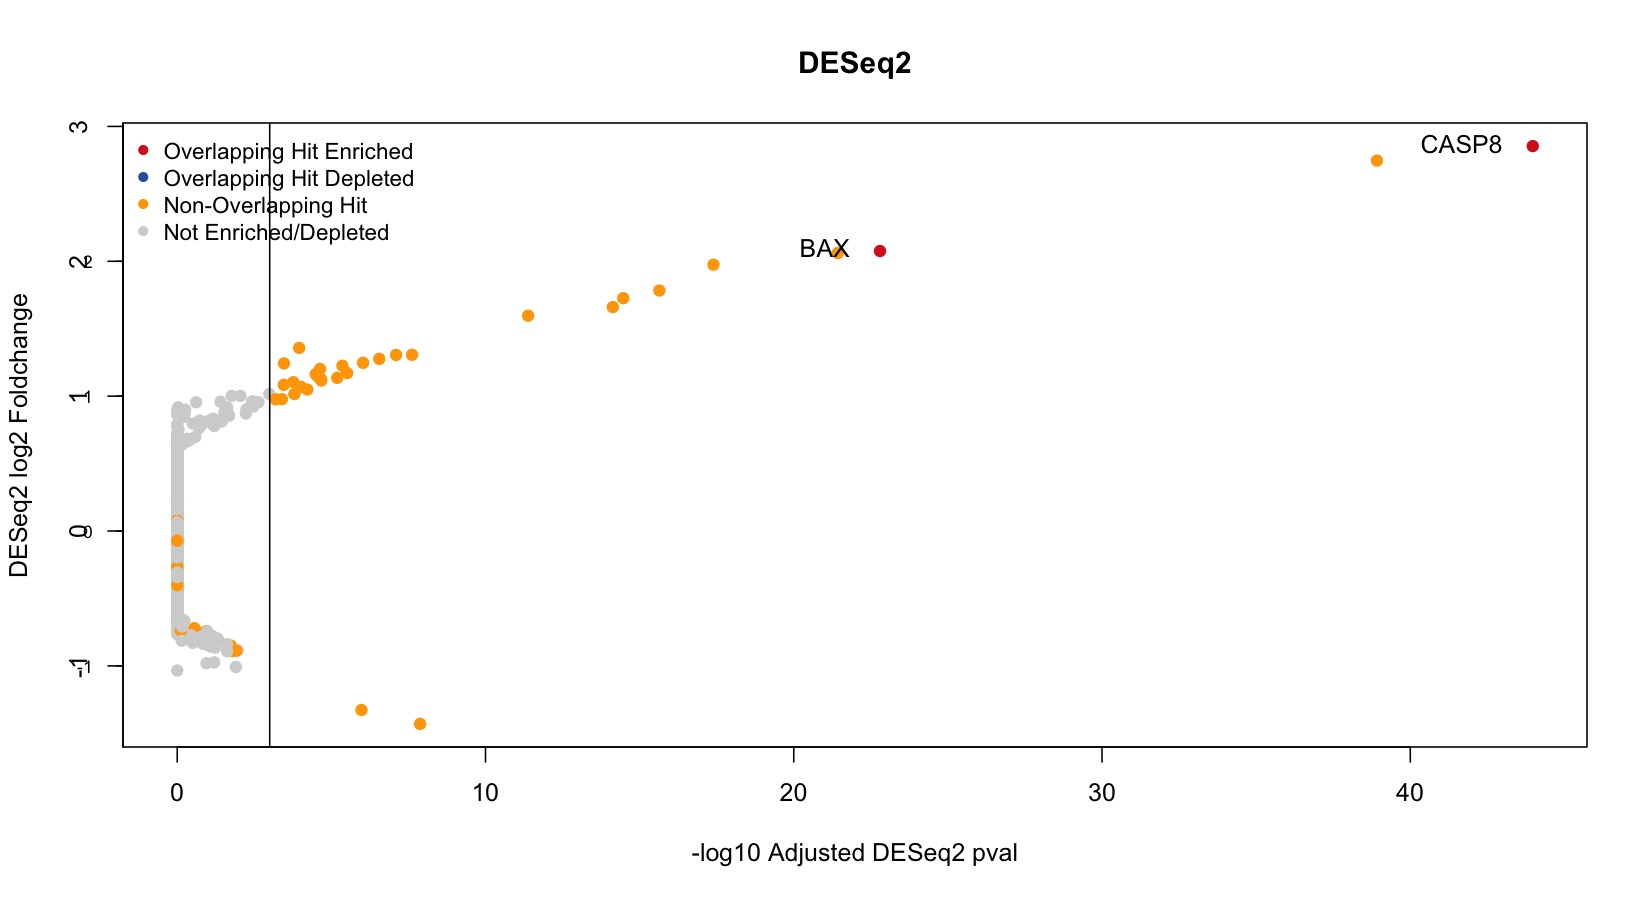
\includegraphics{CaRpools_files/figure-latex/HT-overview-hits-1.pdf}

\paragraph{carpools.hit.overview()}\label{carpools.hit.overview}

\textbf{Usage}\\
\texttt{carpools.hit.overview(wilcox=NULL,\ deseq=NULL,\ mageck=NULL,\ cutoff.deseq\ =\ 0.001,\ cutoff.wilcox\ =\ 0.05,\ cutoff.mageck\ =\ 0.05,\ cutoff.override=FALSE,\ cutoff.hits=NULL,\ plot.genes="overlapping",\ type="all")}

\textbf{wilcox}\\
Data output from \texttt{stat.wilcox}.\\
\emph{Default} NULL\\
\emph{Values} Data output from \texttt{stat.wilcox}.

\textbf{deseq}\\
Data output from \texttt{stat.deseq}.\\
\emph{Default} NULL\\
\emph{Values} Data output from \texttt{stat.deseq}.

\textbf{mageck}\\
Data output from \texttt{stat.mageck}.\\
\emph{Default} NULL\\
\emph{Values} Data output from \texttt{stat.mageck}.

\textbf{cutoff.deseq}\\
P-Value threshold used to determine significance.\\
\emph{Default} 0.001\\
\emph{Values} numeric

\textbf{cutoff.wilcox}\\
P-Value threshold used to determine significance.\\
\emph{Default} 0.001\\
\emph{Values} numeric

\textbf{cutoff.mageck}\\
P-Value threshold used to determine significance.\\
\emph{Default} 0.001\\
\emph{Values} numeric

\textbf{cutoff.override}\\
Shall the p-value threshold be ignored? If this is TRUE, the top
percentage gene of \texttt{cutoff.hits} is used instead.\\
\emph{Default} FALSE\\
\emph{Values} TRUE, FALSE

\textbf{cutoff.hits}\\
The percentatge of top genes being used if
\texttt{cutoff.override=TRUE}.\\
*Default** NULL\\
\emph{Values} numeric

\textbf{plot.genes}\\
Defines what kind of data is used. By default, overlapping genes are
highlighted in red color.\\
\emph{Default} ``overlapping''\\
\emph{Values} ``overlapping''

\textbf{type}\\
Defines whether all genes are plotted or only those being enriched or
depleted.\\
\emph{Default} ``all''\\
\emph{Values} ``all'', ``enriched'', ``depleted''

\subsubsection{Creating VENN Diagrams}\label{creating-venn-diagrams}

CaRpools can also be used to create Venn Diagrams of the top candidates,
thus allowing to see the performance of the analysis methods on your
data set using \texttt{compare.analysis}.\\
Therefore, the package \texttt{VennDiagram} must be imported.

You can plot a Venn Diagram of all enriched hits like this:

\begin{Shaded}
\begin{Highlighting}[]
\NormalTok{venn.enriched =}\StringTok{ }\KeywordTok{compare.analysis}\NormalTok{(}\DataTypeTok{wilcox=}\NormalTok{data.wilcox, }\DataTypeTok{deseq=}\NormalTok{data.deseq, }\DataTypeTok{mageck=}\NormalTok{data.mageck, }\DataTypeTok{type=}\StringTok{"enriched"}\NormalTok{, }\DataTypeTok{cutoff.deseq =} \FloatTok{0.001}\NormalTok{, }\DataTypeTok{cutoff.wilcox =} \FloatTok{0.05}\NormalTok{, }\DataTypeTok{cutoff.mageck =} \FloatTok{0.05}\NormalTok{, }\DataTypeTok{cutoff.override=}\OtherTok{FALSE}\NormalTok{, }\DataTypeTok{cutoff.hits=}\OtherTok{NULL}\NormalTok{, }\DataTypeTok{output=}\StringTok{"venn"}\NormalTok{)}
\KeywordTok{require}\NormalTok{(VennDiagram)}
\end{Highlighting}
\end{Shaded}

\begin{verbatim}
## Loading required package: VennDiagram
## Loading required package: grid
\end{verbatim}

\begin{Shaded}
\begin{Highlighting}[]
\KeywordTok{plot.new}\NormalTok{()}
\NormalTok{grid::}\KeywordTok{grid.draw}\NormalTok{(VennDiagram::}\KeywordTok{venn.diagram}\NormalTok{(venn.enriched, }\DataTypeTok{file=}\OtherTok{NULL}\NormalTok{, }\DataTypeTok{fill=}\KeywordTok{c}\NormalTok{(}\StringTok{"lightgreen"}\NormalTok{,}\StringTok{"lightblue2"}\NormalTok{,}\StringTok{"lightgray"}\NormalTok{), }\DataTypeTok{na=}\StringTok{"remove"}\NormalTok{, }\DataTypeTok{cex=}\DecValTok{2}\NormalTok{,}\DataTypeTok{lty=}\DecValTok{2}\NormalTok{, }\DataTypeTok{cat.cex=}\DecValTok{2}\NormalTok{))}
\end{Highlighting}
\end{Shaded}

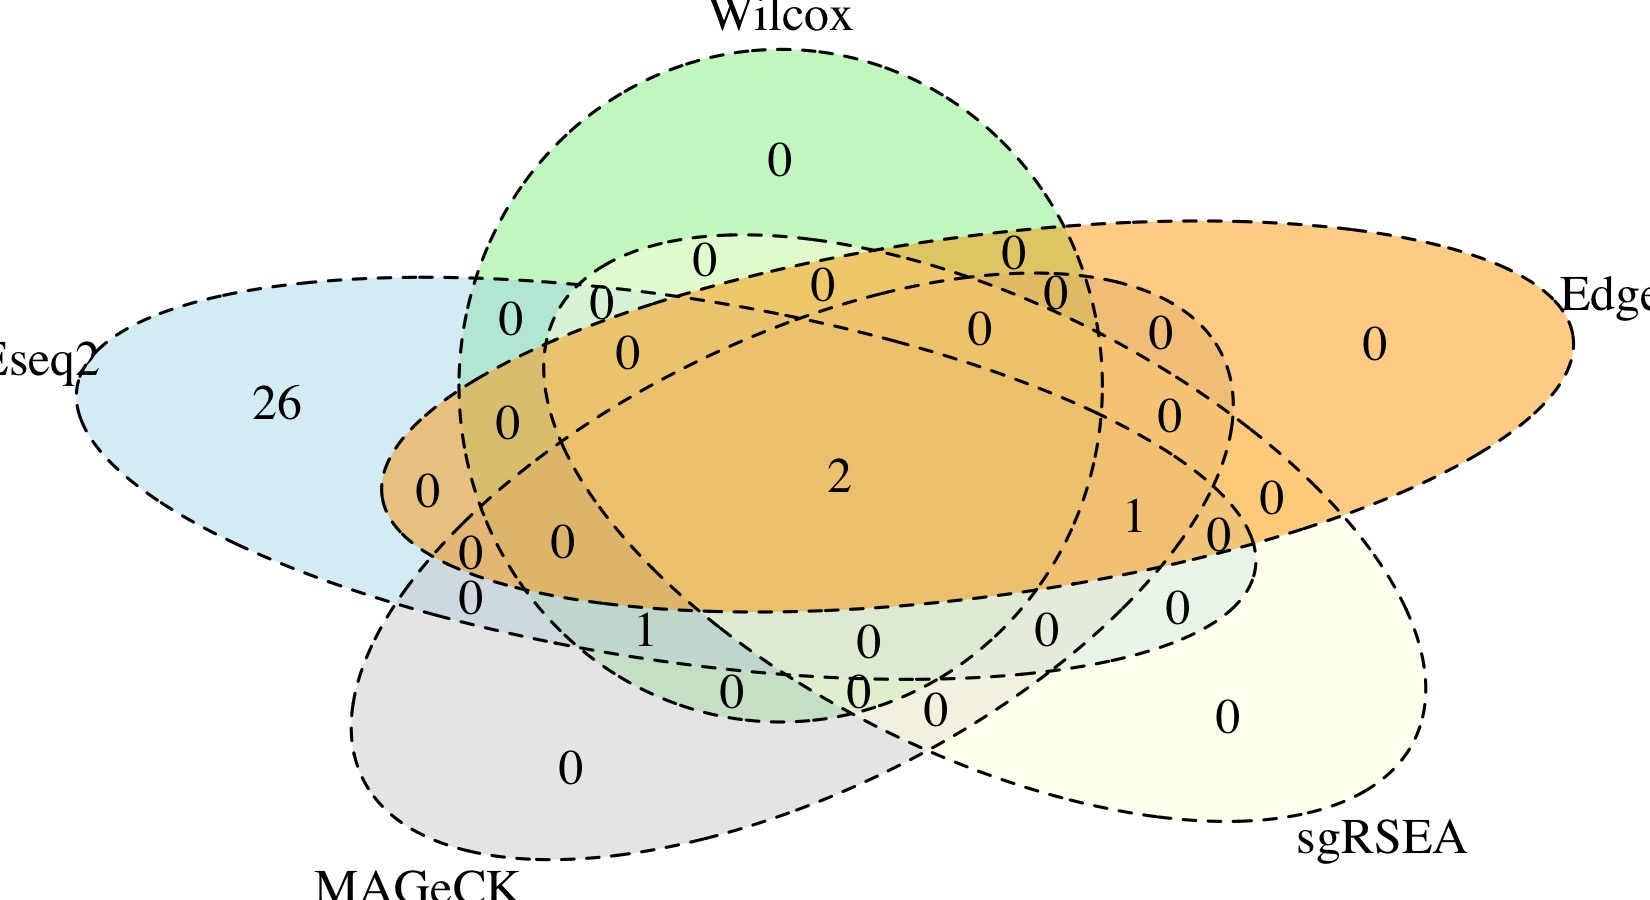
\includegraphics{CaRpools_files/figure-latex/HT-compare-enriched-overlap-1.pdf}

This diagram shows you, that DESeq2 found 41 significantly enriched
genes, out of which 4 where identified voth by Wilcox and MAGeCK.
Moreover, all found candidates by MAGeCK and Wilcox are the same and
included within the DESEq2 ones.

\newpage

\subsection{Export Hit Candidate
Lists}\label{export-hit-candidate-lists}

Although the candidate lists of each analysis method can be saved
separately, caRpools offer a comparative approach, which creates tables
that include the information from all analysis methods at once for a
faster overview.

This is done using the function \texttt{compare.analysis}, which offers
not only ouptu for Venn Diagrams, but also for tables.

\paragraph{Tabular Output with all
information}\label{tabular-output-with-all-information}

You can store the information of all enriched genes with the fold change
and p-value information at once. Moreover, you can select how it is
sorted:

\begin{Shaded}
\begin{Highlighting}[]
\CommentTok{# Perform the comparison}
\NormalTok{data.analysis.enriched =}\StringTok{ }\KeywordTok{compare.analysis}\NormalTok{(}\DataTypeTok{wilcox=}\NormalTok{data.wilcox,}
    \DataTypeTok{deseq=}\NormalTok{data.deseq, }\DataTypeTok{mageck=}\NormalTok{data.mageck, }\DataTypeTok{type=}\StringTok{"enriched"}\NormalTok{,}
    \DataTypeTok{cutoff.override =} \OtherTok{FALSE}\NormalTok{, }\DataTypeTok{cutoff.hits=}\OtherTok{NULL}\NormalTok{, }\DataTypeTok{output=}\StringTok{"list"}\NormalTok{,}
    \DataTypeTok{sort.by=}\KeywordTok{c}\NormalTok{(}\StringTok{"mageck"}\NormalTok{,}\StringTok{"fdr"}\NormalTok{,}\StringTok{"rank"}\NormalTok{))}
\NormalTok{## Write to a file}
\NormalTok{xlsx::}\KeywordTok{write.xlsx}\NormalTok{(data.analysis.enriched,}
    \DataTypeTok{file=}\StringTok{"COMPARE-HITS.xls"}\NormalTok{,}
    \DataTypeTok{sheetName=}\StringTok{"Enriched"}\NormalTok{)}
\CommentTok{# Print to console}
\NormalTok{knitr::}\KeywordTok{kable}\NormalTok{(data.analysis.enriched[}\DecValTok{1}\NormalTok{:}\DecValTok{10}\NormalTok{,}\KeywordTok{c}\NormalTok{(}\DecValTok{2}\NormalTok{:}\DecValTok{7}\NormalTok{)])}
\end{Highlighting}
\end{Shaded}

\begin{longtable}[c]{@{}lrrrrrr@{}}
\toprule
& wilcox.log2fc & wilcox.pval & deseq.log2fc & deseq.pval & mageck.fdr &
mageck.rank\tabularnewline
\midrule
\endhead
CASP8 & 2.8382733 & 0.0178241 & 2.9429395 & 0.0000000 & 0.001650 &
1\tabularnewline
BAX & 2.4706303 & 0.0178241 & 2.1350701 & 0.0000000 & 0.001650 &
2\tabularnewline
FADD & 2.8332735 & 0.0184341 & 2.8317727 & 0.0000000 & 0.001650 &
3\tabularnewline
PASK & 1.3650980 & 0.0178241 & 1.3366397 & 0.0000000 & 0.003713 &
4\tabularnewline
TYRO3 & 1.0116807 & 0.9671744 & 0.6686189 & 0.3923318 & 0.659241 &
5\tabularnewline
AMHR2 & 1.4654422 & 0.9671744 & 1.6291193 & 0.0000000 & 0.659241 &
6\tabularnewline
FN3K & 1.4685534 & 0.4030853 & 1.2532816 & 0.0000000 & 0.661245 &
7\tabularnewline
PRKY & 1.2424191 & 0.9671744 & 1.1942455 & 0.0000001 & 0.785149 &
8\tabularnewline
CDK5RAP3 & 0.8994121 & 0.4202992 & 0.6831604 & 0.0938068 & 0.785149 &
9\tabularnewline
ROR2 & 0.6903593 & 0.9671744 & 0.4210292 & 1.0000000 & 0.785149 &
10\tabularnewline
\bottomrule
\end{longtable}

By default, data is sorted by the gene rank MAGeCK uses.

\paragraph{Rank-based Output}\label{rank-based-output}

Moreover, you can create a table which gives you the rank of a gene
within each analysis method rather than p-value or fold changes. You can
do this by choosing \texttt{output="rank"}.

\begin{Shaded}
\begin{Highlighting}[]
\CommentTok{# Perform the comparison}
\NormalTok{data.analysis.enriched =}\StringTok{ }\KeywordTok{compare.analysis}\NormalTok{(}\DataTypeTok{wilcox=}\NormalTok{data.wilcox,}
    \DataTypeTok{deseq=}\NormalTok{data.deseq, }\DataTypeTok{mageck=}\NormalTok{data.mageck, }\DataTypeTok{type=}\StringTok{"enriched"}\NormalTok{,}
    \DataTypeTok{cutoff.override =} \OtherTok{FALSE}\NormalTok{, }\DataTypeTok{cutoff.hits=}\OtherTok{NULL}\NormalTok{, }\DataTypeTok{output=}\StringTok{"rank"}\NormalTok{,}
    \DataTypeTok{sort.by=}\KeywordTok{c}\NormalTok{(}\StringTok{"mageck"}\NormalTok{,}\StringTok{"fdr"}\NormalTok{,}\StringTok{"rank"}\NormalTok{))}
\NormalTok{## Write to a file}
\NormalTok{xlsx::}\KeywordTok{write.xlsx}\NormalTok{(data.analysis.enriched,}
    \DataTypeTok{file=}\StringTok{"COMPARE-RANKs.xls"}\NormalTok{,}
    \DataTypeTok{sheetName=}\StringTok{"Enriched"}\NormalTok{)}
\CommentTok{# Print to console}
\NormalTok{knitr::}\KeywordTok{kable}\NormalTok{(data.analysis.enriched[}\DecValTok{1}\NormalTok{:}\DecValTok{10}\NormalTok{,])}
\end{Highlighting}
\end{Shaded}

\begin{longtable}[c]{@{}lrrr@{}}
\toprule
& wilcox & deseq & mageck\tabularnewline
\midrule
\endhead
CASP8 & 1 & 1 & 1\tabularnewline
BAX & 3 & 3 & 2\tabularnewline
FADD & 2 & 2 & 3\tabularnewline
PASK & 11 & 12 & 4\tabularnewline
TYRO3 & 36 & 85 & 5\tabularnewline
AMHR2 & 6 & 9 & 6\tabularnewline
FN3K & 5 & 16 & 7\tabularnewline
PRKY & 16 & 19 & 8\tabularnewline
CDK5RAP3 & 60 & 83 & 9\tabularnewline
ROR2 & 131 & 170 & 10\tabularnewline
\bottomrule
\end{longtable}

\paragraph{3D Plot Output}\label{d-plot-output}

You can also create 3D scatterplot view of the overlapping hits by
choosing \texttt{output="3dplot"}. Please not the additional arguments
\texttt{plot.method} and \texttt{plot.feature}, which define what to
plot on each axis.

\begin{Shaded}
\begin{Highlighting}[]
\CommentTok{# Perform the comparison and create 3D plot only for enriched}
\NormalTok{compared =}\StringTok{ }\KeywordTok{compare.analysis}\NormalTok{( }\DataTypeTok{wilcox=}\NormalTok{data.wilcox, }\DataTypeTok{deseq=}\NormalTok{data.deseq, }\DataTypeTok{mageck=}\NormalTok{data.mageck, }\DataTypeTok{type=}\StringTok{"enriched"}\NormalTok{, }\DataTypeTok{cutoff.deseq =} \FloatTok{0.001}\NormalTok{, }\DataTypeTok{cutoff.wilcox =} \FloatTok{0.05}\NormalTok{, }\DataTypeTok{cutoff.mageck =} \FloatTok{0.05}\NormalTok{, }\DataTypeTok{cutoff.override=}\OtherTok{FALSE}\NormalTok{, }\DataTypeTok{cutoff.hits=}\OtherTok{NULL}\NormalTok{, }\DataTypeTok{output=}\StringTok{"3dplot"}\NormalTok{, }\DataTypeTok{sort.by=}\KeywordTok{c}\NormalTok{(}\StringTok{"mageck"}\NormalTok{,}\StringTok{"rank"}\NormalTok{,}\StringTok{"rank"}\NormalTok{), }\DataTypeTok{plot.method=}\KeywordTok{c}\NormalTok{(}\StringTok{"wilcox"}\NormalTok{,}\StringTok{"deseq"}\NormalTok{,}\StringTok{"mageck"}\NormalTok{), }\DataTypeTok{plot.feature=}\KeywordTok{c}\NormalTok{(}\StringTok{"pval"}\NormalTok{,}\StringTok{"pval"}\NormalTok{,}\StringTok{"fdr"}\NormalTok{))}
\end{Highlighting}
\end{Shaded}

\includegraphics{CaRpools_files/figure-latex/HT-comparetable-enriched-3d-1.pdf}

\paragraph{compare.analysis()}\label{compare.analysis}

\textbf{Usage}
\texttt{compare.analysis(wilcox=NULL,\ deseq=NULL,\ mageck=NULL,\ type="enriched",\ cutoff.deseq\ =\ NULL,\ cutoff.wilcox\ =\ NULL,\ cutoff.mageck\ =\ NULL,\ cutoff.override=TRUE,\ cutoff.hits=5,\ output="list",\ sort.by=c("mageck","fdr","fdr"),\ plot.method=c("wilcox","mageck",\ "deseq"),\ plot.feature=c("pval","fdr","pval"),\ pch=16)}

\textbf{wilcox}\\
Data output from \texttt{stat.wilcox}.\\
\emph{Default} NULL\\
\emph{Values} Data output from \texttt{stat.wilcox}.

\textbf{deseq}\\
Data output from \texttt{stat.deseq}.\\
\emph{Default} NULL\\
\emph{Values} Data output from \texttt{stat.deseq}.

\textbf{mageck}\\
Data output from \texttt{stat.mageck}.\\
\emph{Default} NULL\\
\emph{Values} Data output from \texttt{stat.mageck}.

\textbf{cutoff.deseq}\\
P-Value threshold used to determine significance.\\
\emph{Default} 0.001\\
\emph{Values} numeric

\textbf{cutoff.wilcox}\\
P-Value threshold used to determine significance.\\
\emph{Default} 0.001\\
\emph{Values} numeric

\textbf{cutoff.mageck}\\
P-Value threshold used to determine significance.\\
\emph{Default} 0.001\\
\emph{Values} numeric

\textbf{cutoff.override}\\
Shall the p-value threshold be ignored? If this is TRUE, the top
percentage gene of \texttt{cutoff.hits} is used instead.\\
\emph{Default} FALSE\\
\emph{Values} TRUE, FALSE

\textbf{cutoff.hits}\\
The percentatge of top genes being used if
\texttt{cutoff.override=TRUE}.\\
*Default** NULL\\
\emph{Values} numeric

\textbf{output}\\
Three different types of output can be generated: A list with all genes
including the information from \texttt{stat.wilcox}, \texttt{stat.DEseq}
and \texttt{stat.mageck}, a sorted ranked output, a venn diagram
compatible output and 3D scatterplot.\\
\emph{Default} ``list''\\
\emph{Values} ``list'', ``rank'', ``venn'', ``3dplot''

\textbf{sort.by}\\
This indicates the sorting for \texttt{type="rank"\ and\ type="list"}
and is a vector. By default, data is sorted by the FDR of MAGeCK. needs
to be a vector.\\
\emph{Default} c(``mageck'',``fdr'',``fdr'')\\
\emph{Values} c(``mageck'',``fdr'',``fdr''),
c(``mageck'',``fdr'',``rank''), c(``mageck'',``fdr'',``rank''),
c(``wilcox'',``pval'',``pval''), c(``wilcox'',``pval'',``genes''),
c(``deseq'',``pval'',``pval''), c(``deseq'',``pval'',``genes'')

\textbf{plot.method}\\
Used only if \texttt{type="3dplot"}. This indicates what is plotted at
the x, y and z-axis and thus needs to be a vector of length 3.\\
\emph{Default} c(``wilcox'',``mageck'', ``deseq''), plots wilcox on
X-axis, mageck on y-axis and deseq on z-axis\\
\emph{Values} c(``wilcox'',``mageck'', ``deseq'') or any other
combination

\textbf{plot.feature}\\
If \texttt{type="3dplot"}, this indicates the type of data plotted on
each axis of the 3d plot. This can only be set according to the features
available of the method used to be plotted as indicated in
\texttt{plot.method}.\\
\emph{Default} c(``pval'',``fdr'', ``pval'') which uses the p-value of
wilcox, the fdr or MAGeCK and p-value of DESeq2.\\
\emph{Values} c(``pval'',``fdr'', ``pval''), or ANY combination
according to \texttt{plot.method}

\newpage

\subsection{Creating Final Hit Candidate
Table}\label{creating-final-hit-candidate-table}

CaRpools also provides you with a final gene table, which includes
p-values, fold changes and ranks by all methods in a single tabular
output.\\
This output is \textbf{unbiased} and can thus be used for further
analysis and data visualization.\\
It takes the output generated by each analysis method,
\texttt{stat.wilcox}, \texttt{stat.DEseq} and \texttt{stat.mageck} and
combines it into a single tabular representation.

\begin{Shaded}
\begin{Highlighting}[]
\CommentTok{# create final table with all genes + hit analysis results}
\NormalTok{final.tab =}\StringTok{ }\KeywordTok{final.table}\NormalTok{(}\DataTypeTok{wilcox=}\NormalTok{data.wilcox, }\DataTypeTok{deseq=}\NormalTok{data.deseq, }\DataTypeTok{mageck=}\NormalTok{data.mageck, }\DataTypeTok{dataset=}\NormalTok{CONTROL1.g, }\DataTypeTok{namecolumn=}\DecValTok{1}\NormalTok{, }\DataTypeTok{type=}\StringTok{"genes"}\NormalTok{)}

\CommentTok{# Write this to an EXCEL sheet}
\NormalTok{xlsx::}\KeywordTok{write.xlsx}\NormalTok{(final.tab, }\StringTok{"FINAL.xls"}\NormalTok{, }\DataTypeTok{sheetName=}\StringTok{"Genelist"}\NormalTok{, }
  \DataTypeTok{col.names=}\OtherTok{TRUE}\NormalTok{, }\DataTypeTok{row.names=}\OtherTok{FALSE}\NormalTok{, }\DataTypeTok{append=}\OtherTok{FALSE}\NormalTok{, }\DataTypeTok{showNA=}\OtherTok{TRUE}\NormalTok{)}
\end{Highlighting}
\end{Shaded}

An example of the generated output:

\begin{longtable}[c]{@{}lrrrrrrr@{}}
\toprule
name & wilcox.FC & wilcox.pval & deseq2.pval & mageck.rank.pos &
mageck.fdr.pos & mageck.rank.neg & mageck.fdr.neg\tabularnewline
\midrule
\endhead
AAK1 & 0.4487116 & 0.9802939 & 1 & 354 & 0.987129 & 744 &
0.994232\tabularnewline
AATK & 0.4542620 & 0.9802939 & 1 & 426 & 0.987129 & 88 &
0.973911\tabularnewline
ABI1 & 0.5490720 & 0.9671744 & 1 & 356 & 0.987129 & 764 &
0.994232\tabularnewline
ABL1 & 0.2882981 & 0.9802939 & 1 & 679 & 0.996304 & 320 &
0.993066\tabularnewline
ABL2 & 0.8073053 & 1.0000000 & 1 & 100 & 0.987129 & 302 &
0.993066\tabularnewline
ACAD10 & 0.1910946 & 0.9802939 & 1 & 641 & 0.996304 & 659 &
0.994232\tabularnewline
ACVR1 & 0.2899392 & 1.0000000 & 1 & 293 & 0.987129 & 171 &
0.993066\tabularnewline
ACVR1B & 0.0286973 & 0.9820183 & 1 & 805 & 0.996304 & 268 &
0.993066\tabularnewline
ACVR1C & 0.2157256 & 1.0000000 & 1 & 580 & 0.996304 & 541 &
0.994232\tabularnewline
ACVR2A & 0.3923660 & 1.0000000 & 1 & 314 & 0.987129 & 516 &
0.994232\tabularnewline
ACVR2B & 0.4256165 & 0.9802939 & 1 & 618 & 0.996304 & 655 &
0.994232\tabularnewline
ACVRL1 & 0.2157440 & 0.9802939 & 1 & 651 & 0.996304 & 40 &
0.808760\tabularnewline
ADAM9 & 0.2736503 & 0.9820183 & 1 & 481 & 0.987129 & 767 &
0.994232\tabularnewline
ADCK1 & 0.7768593 & 0.9671744 & 1 & 105 & 0.987129 & 544 &
0.994232\tabularnewline
ADCK2 & 0.3940072 & 0.9820183 & 1 & 509 & 0.987129 & 64 &
0.973911\tabularnewline
ADCK4 & 0.1430250 & 0.9802939 & 1 & 593 & 0.996304 & 309 &
0.993066\tabularnewline
ADCK5 & 0.0257506 & 1.0000000 & 1 & 748 & 0.996304 & 667 &
0.994232\tabularnewline
ADK & 0.4217891 & 1.0000000 & 1 & 317 & 0.987129 & 220 &
0.993066\tabularnewline
ADRA1A & 0.3570135 & 1.0000000 & 1 & 413 & 0.987129 & 437 &
0.994232\tabularnewline
ADRA1B & 0.4534786 & 1.0000000 & 1 & 470 & 0.987129 & 381 &
0.994232\tabularnewline
\bottomrule
\end{longtable}

\paragraph{final.table()}\label{final.table}

\textbf{Usage}\\
\texttt{final.table(wilcox=NULL,\ deseq=NULL,\ mageck=NULL,\ dataset,\ namecolumn=1,\ norm.function=median,\ type="genes",\ extractpattern\ =\ expression("\^{}(.+?)\_.+"))}

\textbf{wilcox}\\
Data output from \texttt{stat.wilcox}.\\
\emph{Default} NULL\\
\emph{Values} Data output from \texttt{stat.wilcox}.

\textbf{deseq}\\
Data output from \texttt{stat.deseq}.\\
\emph{Default} NULL\\
\emph{Values} Data output from \texttt{stat.deseq}.

\textbf{mageck}\\
Data output from \texttt{stat.mageck}.\\
\emph{Default} NULL\\
\emph{Values} Data output from \texttt{stat.mageck}.

\textbf{dataset}\\
Data.frame as created by \texttt{load.file}\\
\emph{Default} empty\\
\emph{Values} data frame

\textbf{namecolumn}\\
In which column are the sgRNA identifiers?\\
\emph{Default} 1\\
\emph{Values} column number (numeric)

\textbf{extractpattern}\\
PERL regular expression that is used to retrieve the gene identifier
from the overall sgRNA identifier.\\
e.g.~in \textbf{AAK1\_107\_0} it will extract \textbf{AAK1}, since this
is the gene identifier beloning to this sgRNA identifier. \textbf{Please
see: Read-Count Data Files}\\
\emph{Default} expression(``\^{}(.+?)(\_.+)``), will work for most
available libraries.\\
\emph{Values} PERL regular expression with parenthesis indicating the
gene identifier (expression)

\textbf{norm.function}\\
The mathematical function to normalize data if \texttt{normalize=TRUE}.
By default, the median is used.\\
\emph{Default} median\\
\emph{Values} Any mathematical function of R (function)

\subsubsection{Create List of Overlapping Hit
Candidates}\label{create-list-of-overlapping-hit-candidates}

CaRpools can also calculate which genes overlapped in all hit analysis
methods using \texttt{generate.hits}.

\begin{Shaded}
\begin{Highlighting}[]
\NormalTok{overlap.enriched =}\StringTok{ }\KeywordTok{generate.hits}\NormalTok{(}\DataTypeTok{wilcox=}\NormalTok{data.wilcox, }\DataTypeTok{deseq=}\NormalTok{data.deseq, }\DataTypeTok{mageck=}\NormalTok{data.mageck, }\DataTypeTok{type=}\StringTok{"enriched"}\NormalTok{, }\DataTypeTok{cutoff.deseq =} \FloatTok{0.001}\NormalTok{, }\DataTypeTok{cutoff.wilcox =} \FloatTok{0.05}\NormalTok{, }\DataTypeTok{cutoff.mageck =} \FloatTok{0.05}\NormalTok{, }\DataTypeTok{cutoff.override=}\OtherTok{FALSE}\NormalTok{, }\DataTypeTok{cutoff.hits=}\OtherTok{NULL} \NormalTok{, }\DataTypeTok{plot.genes=}\StringTok{"overlapping"}\NormalTok{)}
\end{Highlighting}
\end{Shaded}

\begin{longtable}[c]{@{}l@{}}
\toprule
CASP8\tabularnewline
BAX\tabularnewline
FADD\tabularnewline
PASK\tabularnewline
\bottomrule
\end{longtable}

\paragraph{generate.hits()}\label{generate.hits}

\textbf{Usage}\\
\texttt{generate.hits(wilcox=NULL,\ deseq=NULL,\ mageck=NULL,\ \ type="enriched",\ cutoff.deseq\ =\ 0.001,\ cutoff.wilcox\ =\ 0.05,\ cutoff.mageck\ =\ 0.05,\ cutoff.override=FALSE,\ cutoff.hits=NULL,\ plot.genes="overlapping")}

\textbf{wilcox}\\
Data output from \texttt{stat.wilcox}.\\
\emph{Default} NULL\\
\emph{Values} Data output from \texttt{stat.wilcox}.

\textbf{deseq}\\
Data output from \texttt{stat.deseq}.\\
\emph{Default} NULL\\
\emph{Values} Data output from \texttt{stat.deseq}.

\textbf{mageck}\\
Data output from \texttt{stat.mageck}.\\
\emph{Default} NULL\\
\emph{Values} Data output from \texttt{stat.mageck}.

\textbf{cutoff.deseq}\\
P-Value threshold used to determine significance.\\
\emph{Default} 0.001\\
\emph{Values} numeric

\textbf{cutoff.wilcox}\\
P-Value threshold used to determine significance.\\
\emph{Default} 0.001\\
\emph{Values} numeric

\textbf{cutoff.mageck}\\
P-Value threshold used to determine significance.\\
\emph{Default} 0.001\\
\emph{Values} numeric

\textbf{cutoff.override}\\
Shall the p-value threshold be ignored? If this is TRUE, the top
percentage gene of \texttt{cutoff.hits} is used instead.\\
\emph{Default} FALSE\\
\emph{Values} TRUE, FALSE

\textbf{cutoff.hits}\\
The percentatge of top genes being used if
\texttt{cutoff.override=TRUE}.\\
*Default** NULL\\
\emph{Values} numeric

\textbf{plot.genes}\\
Defines what kind of data is returned, by default only overlapping genes
or MAGeCK.\\
\emph{Default} ``overlapping''\\
\emph{Values} ``overlapping''

\section{Further Information}\label{further-information}

Please have a look at \href{http://www.crispr-analyzer.de}{our website}
where you can find manuals, pre-defined reports, all scripts mentioned
in this manual and a bug-tracker.\\
If you like to use or modify any of the code of caRpools, please fork or
clone the github repository. If you find any bug or if you have a clever
idea that you would like to have it included in caRpools, feel free to
code or dropt us a comment.

\end{document}
